\documentclass[10pt,a4paper]{article}
\usepackage[UTF8,fontset = windows]{ctex}
\setCJKmainfont[BoldFont=黑体,ItalicFont=楷体]{华文中宋}
\usepackage{amssymb,amsmath,amsfonts,amsthm,mathrsfs,dsfont,graphicx}
\usepackage{ifthen,indentfirst,enumerate,color,titletoc}
\usepackage{tikz}
\usepackage{makecell}
\usetikzlibrary{arrows,calc,intersections,patterns}
\usepackage[bf,small,indentafter,pagestyles]{titlesec}
\usepackage[top=1in, bottom=1in,left=0.8in,right=0.8in]{geometry}
\renewcommand{\baselinestretch}{1.65}
\newtheorem{defi}{定义~}
\newtheorem{eg}{例~}
\newtheorem{ex}{~}
\newtheorem{rem}{注~}
\newtheorem{thm}{定理~}
\newtheorem{coro}{推论~}
\newtheorem{axiom}{公理~}
\newtheorem{prop}{性质~}
\newcommand{\blank}[1]{\underline{\hbox to #1pt{}}}
\newcommand{\bracket}[1]{(\hbox to #1pt{})}
\newcommand{\onech}[4]{\par\begin{tabular}{p{.9\textwidth}}
A.~#1\\
B.~#2\\
C.~#3\\
D.~#4
\end{tabular}}
\newcommand{\twoch}[4]{\par\begin{tabular}{p{.46\textwidth}p{.46\textwidth}}
A.~#1& B.~#2\\
C.~#3& D.~#4
\end{tabular}}
\newcommand{\vartwoch}[4]{\par\begin{tabular}{p{.46\textwidth}p{.46\textwidth}}
(1)~#1& (2)~#2\\
(3)~#3& (4)~#4
\end{tabular}}
\newcommand{\fourch}[4]{\par\begin{tabular}{p{.23\textwidth}p{.23\textwidth}p{.23\textwidth}p{.23\textwidth}}
A.~#1 &B.~#2& C.~#3& D.~#4
\end{tabular}}
\newcommand{\varfourch}[4]{\par\begin{tabular}{p{.23\textwidth}p{.23\textwidth}p{.23\textwidth}p{.23\textwidth}}
(1)~#1 &(2)~#2& (3)~#3& (4)~#4
\end{tabular}}
\begin{document}
\begin{enumerate}[1.]
% 第一讲 8+3+7
\item 用适当符号($\in$, $\notin$, $=$, $\subsetneqq$)填空:$\pi$\blank{10}$\mathbf{Q}$; $\{x|x=2k+1, \ k\in \mathbf{Z}\}$\blank{10}$\{x|x=2k-1,k\in \mathbf{Z}\}$; $\{3.14\}$\blank{10}$\mathbf{Q}$; $\{y|y=x^2\}$\blank{10}$\{x|y=x^2\}$.  
\item 已知$P=\{y=x^2+1\}$, $Q=\{y|y=x^2+1, \ x\in \mathbf{R}\}$, $E=\{x|y=x^2+1, \  x\in \mathbf{R}\}$, $F=\{(x,y)|y=x^2+1, \ x\in \mathbf{R}\}$, $G=\{x|x\ge 1\}$, $H=\{x|x^2+1=0, \ x\in \mathbf{R}\}$, 则各集合间关系正确的有\blank{50}. (答案可能不唯一)\\
(A) $P=F$   (B) $Q=E$   (C) $E=F$   (D) $Q\subseteq G$  (E) $H\subsetneqq P$
\item 设全集是实数集$\mathbf{R}$, $M=\{x|-2 \le x\le 2\}$, $N=\{x|x<1\}$, 则$\complement_U M\cap N=$\blank{50}.
\item 设$A=\{x|-4<x<4, \ x\in \mathbf{R}\}$, $B=(-\infty,1]\cup [3,+\infty)$, 则$\{x|x\in A, \ x\notin A\cap B  \}$=\blank{50}.
\item 设$A=\{x|x=\sqrt k, \ k\in \mathbf{N}\}$,$B=\{x|x\le 3,\ x\in \mathbf{Q}\}$, 则$A\cap B=$\blank{50}.
\item 设全集$U=\{2,3,a^2+2a-3\}$, 集合$A=\{|2a-1|,2\}$, $\complement_U A=\{5\}$, 则实数$a=$\blank{50}.
\item (1) 设$M=\{y|y=x^2, x\in \mathbf{R}\}$, $N=\{x|x=t,\ t\in \mathbf{R}\}$, 则$M\cap N=$\blank{50}.\\
(2) 设$M=\{(x,y)|y=x^2,\ x\in \mathbf{R}\}$, $N=\{(t,x)|x=t,\ t\in \mathbf{R}\}$, 则$M\cap N=$\blank{50}.
\item 设全集$U=\{1,2,3,4\}$, $\complement_U A\cap B=\{3\}$, $A\cap \complement_U B=\{2\}$, $\complement_U A\cup \complement_U B=\{2,3,4\}$, 则$\complement_U A\cap \complement_U B=$\blank{50}.
\item 集合$C=\{x|x=\dfrac k2\pm \dfrac14, \ k\in \mathbf{Z}\},D=\{x|x=\dfrac k4,\ k\in \mathbf{Z}\}$, 试判断$C$与$D$的关系, 并证明.
\item 集合$A=\{x|x^2+4x=0\}$, $B=\{x|x^2+2(a+1)x+a^2-1=0,\ x\in \mathbf{R}\}$.\\
(1) 若$A\cap B=A$, 求实数$a$的取值范围;\\
(2) 若$A\cup B=A$, 求实数$a$的取值范围.
\item 若集合$A=[2,3]$, 集合$B=[a,2a+1]$.\\
(1) 若$A\subsetneqq B$, 求实数$a$的取值范围;\\
(2) 若$A\cap B\ne \varnothing$, 求实数$a$的取值范围.
\item 设全集$U=\mathbf{R}$, 集合$A=\{x|f(x)=0\}$, $B=\{x|g(x)=0\}$, $C=\{x|h(x)=0, \ x\in \mathbf{R}\}$, 则方程$\dfrac{f^2(x)+g^2(x)}{h(x)}=0$的解集是\blank{50}(用$U,A,B,C$表示).
\item (1) 已知集合$A=\{y|y=x^2, \ x\in \mathbf{R}\}, B=\{y|y=4-x^2, \ x\in \mathbf{R}\}$, 则$A\cap B=$\blank{50}.\\
(2) 已知集合$A=\{(x,y)|y={x^2},\ x\in \mathbf{R}\}$, $B=\{(x,y)|y=4-x^2, \ x\in \mathbf{R}\}$, 则$A\cap B=$\blank{50}.
\item 设$m\in \mathbf{R}$, 已知$A=\{x|x^2-3x+2=0\}$, $B=\{x|mx+1=0\}$, 且$B\subsetneqq A$, 则$m=$\blank{50}.
\item (1) 集合$A$满足$\{1\}\subseteq A \subsetneqq \{1,2,3,4\}$, 则满足条件的集合$A$有\blank{50}个.
(2) 若$A\cup B=\{1,2\}$, 将满足条件的集合$A$, $B$写成有序集合对$(A,B)$, 则有序集合对$(A,B)$有\blank{50}个.
\item 已知$A=\{x|x^2-3x+2=0\}$, $B=\{x|x^2-ax+a=0, \ x\in \mathbf{R}\}$, 若$B\subsetneqq A$, 求满足题意的实数$a$.
\item 设集合$A=\{x|x^2+px+1=0,\ x\in \mathbf{R}\}$, 若$A\cap \mathbf{R}^+=\varnothing$. 求实数p的取值范围.
\item 设函数$f(x)=\lg (\dfrac2{x+1}-1)$的定义域为集合$A$, 函数$g(x)=\sqrt{1-|x+a|}$的定义域为集合$B$.\\
(1) 当$a=1$时, 求集合$B$.\\
(2) 问: $a\ge 2$是$A\cap B=\varnothing$的什么条件(在``充分非必要条件、必要非充分条件、充要条件、既非充分也非必要条件''中选一)?并证明你的结论.

% 第二讲 8+3+10

\item 如图, $U$为全集, $M,P,S$是$U$的三个子集, 则阴影部分所表示的集合是\bracket{20}.
\fourch{$(M\cap P)\cap S$}{$(M\cap P)\cup S$}{$(M\cap P)\cap \complement_U S$}{$(M\cap P)\cup \complement_U S$}
\begin{center}
    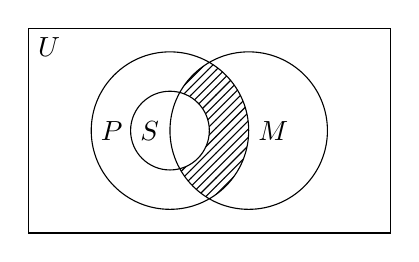
\begin{tikzpicture}
        \begin{scope}
            \clip (1,0) circle (1);
            \begin{scope}[even odd rule]
                \clip (0,0) circle (1) (0,0) circle (0.5);
                \filldraw [pattern = {north east lines}] (-2,-2) rectangle (2,2);
            \end{scope}
        \end{scope}
        \draw (0,0) circle (1) (1,0) circle (1) (0,0) circle (0.5);
        \draw (-1.8,-1.3) rectangle (2.8,1.3);
        \draw (-1.8,1.3) node [below right] {$U$} (-1,0) node [right] {$P$} (-0.5,0) node [right] {$S$} (1,0) node [right] {$M$};
    \end{tikzpicture}
\end{center}
\item 设集合$A=\{5,\log_2(a+3)\}$, $B=\{a,b\}$, 若$A\cap B=\{2\}$, 则$A\cup B=$\blank{50}.
\item 设集合$A\cap \{-2,0,1\}=\{0,1\}$, $A\cup \{-2,0,2\}=\{-2,0,1,2\}$, 则满足上述条件的集合$A$的个数为\blank{50}个.
\item 若集合$A=\{x|x\le 2\}$, $B=\{x|x\ge a\}$, 满足$A\cap B=\{2\}$, 则实数$a=$\blank{50}.
\item 若集合$M=[a-1,a+1]$, $N=(-\infty,-1)\cup [2,+\infty)$, 且$M\cap N=\varnothing$, 则实数$a$的取值范围为\blank{50}.
\item 集合$A=\{(x,y)|x^2+y^2=25\}$, $B=\{(x,y)|x=3y=4\}$, 则$A\cap B$的子集个数是\blank{50}个.
\item 已知集合$M=\{x|x=3m+1, \ m\in \mathbf{Z}\}$, $N=\{y|y=3m+2, \ m\in \mathbf{Z}\}$, 若$x_0\in M$, $y_0\in N$, 则$x_0y_0$与集合$M,N$的关系是\bracket{20}.
\twoch{$x_0y_0\in M$但$x_0y_0$$\notin N$}{$x_0y_0\in N$但$x_0y_0\notin M$}{$x_0y_0\notin M$且$x_0y_0\notin N$}{$x_0y_0$$\in M$且$x_0y_0\in N$}
\item 若$A=\{x|x=2n,\ n\in \mathbf{Z}\}$, $B=\{x|x=4m,\ m\in \mathbf{Z}\}$, 求证:$B\subsetneqq A$.
\item 设常数$a\in \mathbf{R}$, 集合$A=\{x|\dfrac{3-2x}{x-1}+1 \ge 0, \ x\in \mathbf{R}\}$, $B=\{x|2ax<a+x, \ x\in \mathbf{R} \}$.若$A\cup B=B$, 求$a$的取值范围.
\item 设常数$m\in \mathbf{R}$, $A=\{(x,y)|x^2+mx-y+2=0,\ x\in \mathbf{R}\}$, $B=\{(x,y)|x-y+1=0, x\in M\}$, 且$A\cap B\ne\varnothing$.\\
(1) 若$M=\mathbf{R}$, 求实数$m$的取值范围;\\
(2) 若$M=(\dfrac13,2]$, 求实数$m$的取值范围.
\item 设常数$k\in \mathbf{R}$, 关于$x$的不等式组$\begin{cases} x^2-x-2>0, \\ 2x^2+(2k+5)x+5k<0 \end{cases}$ 整数解的集合为$\{-2\}$, 求实数$k$的取值范围.
\item 设$A=\{(x,y)|y=-4x+6,\ x\in \mathbf{R}\}, B=\{(x,y)|y=5x-3,\ x\in \mathbf{R}\}$, 则$A\cap B=$\blank{50}.
\item 已知$M=\{a|\dfrac6{5-a}\in \mathbf{N}, \ a\in \mathbf{Z}\}$, 则用列举法表示$M=$\blank{50}.
\item 定义集合运算: $A\odot B=\{z|z=xy(x+y), \ x\in A, \ y\in B \}$, 设集合$A=\{0,1\}$, $B=\{2,3\}$, 则集合$A\odot B$的所有元素之和为\blank{50}.
\item 已知全集$U=\mathbf{R}$, $A=\{-1\}$, $B=\{x|\lg (x^2-2)=\lg x\}$, 则\bracket{20}
\fourch{$A\subseteq B$}{$A\cup B=\varnothing$}{$A\supseteq B$}{$(\complement_U A)\cap B=\{2\}$}
\item 集合$A=\{(x,y)|y=|x|+1\}$, $B=\{(x,y)|y=\dfrac12x+a\}$, 若$A\cap B=\varnothing$, 则$a$的取值范围是\blank{50}.
\item 调查某班$50$名学生, 音乐爱好者有$40$人, 体育爱好者有$24$人, 则两方面都爱好的人数最少\blank{50}人, 最多\blank{50}人.
\item 已知集合$A=\{x|ax^2-3x+2=0\}$至多有一个元素, 则$a$的取值范围是\blank{50}; 若至少有一个元素, 则$a$的取值范围是\blank{50}.
\item 设含有三个实数的集合既可以表示为$\{a,\dfrac ba,1\}$, 又可以表示为$\{a^2,a+b,0\}$, 那么$a+b=$\blank{50}.
\item 设$f(x)=x^2-12x+36$, $A=\{a|1\le a\le 10, \ a\in \mathbf{N}\}$, $B=\{b|b=f(a),\ a\in A\}$, 又设$C=A\cap B$. 求集合$C$.
\item 设常数$m\in \mathbf{R}$, $A=\{(x,y)|y=-x^2+mx-1,\ x\in \mathbf{R}\}$, $B=\{(x,y)|x+y=3,\ x\in M\}$, 且$A\cap B$的子集有两个.\\
(1) 若$M=\mathbf{R}$, 求实数$m$的值;\\
(2) 若$M=[0,3]$, 求实数$m$的取值范围.

% 第三讲 8+3+8

\item 填写下列命题的否定形式:\\
(1) $m\le 0$或$n>0$: \blank{200};\\
(2) 空间三条直线$l,m,n$两两相交: \blank{200};\\
(3) 复数$z_1,z_2,z_3$中至多一个为纯虚数: \blank{200}.
\item 已知$a,b$是整数, 写出命题``若$ab$为偶数, 则$a+b$为偶数''的逆命题、否命题、逆否命题, 并判断所写命题的真假.\\
逆命题:\blank{200}, 真假: \blank{20};\\
否命题:\blank{200}, 真假: \blank{20};\\
逆否命题:\blank{200}, 真假: \blank{20}.
\item 设甲是乙的充分非必要条件, 乙是丙的充要条件, 丁是丙的必要非充分条件, 则丁是甲的\bracket{20}.
\twoch{充分非必要条件}{必要非充分条件}{充要条件}{既非充分又非必要条件}
\item 若$A$是$B$的必要非充分条件, 则$\overline{A}$是$\overline{B}$的\blank{50}条件.  
\item 下列各组命题中互为等价命题的是\bracket{20}.
\twoch{$A\subseteq B$与$A\cup B=B$}{$x\in A$且$x\in B$与$x\in A\cup B$}{$a\in A\cap B$与$a\in A$或$a\in B$}{$m\in A\cap B$与$m\in A\cup B$}
\item 填空(在``充分不必要''、``必要不充分''、``充要''、``既不充分也不必要''中选一种作答):\\
(1) ``$\alpha \ne \beta$''是$\cos \alpha \ne \cos \beta$''的\blank{50}条件;\\
(2) 在$\triangle ABC$中, ``$A=B$''是``$\sin A=\sin B$''的\blank{50}条件.
\item ``$a>0b>0$''的一个必要非充分条件是\bracket{20}.
\fourch{$a>0$}{$b>0$}{$a>0b>0$}{$a,b\in \mathbf{R}$}
\item ``函数$f(x)\ (x\in \mathbf{R})$存在反函数''是``函数$f(x)$在$\mathbf{R}$上为增函数''的\bracket{20}.
\twoch{充分而不必要条件}{必要而不充分条件}{充分必要条件}{既不充分也不必要条件}
\item 填空: (填``充分不必要''、``必要不充分''、``充要''、``既不充分也不必要'')\\ 
(1) 对于实数$x,y$, $p$: $xy>1$且$x+y>2$是$q$: $x>1$且$y>1$的\blank{50}条件;\\
(2) 对于实数$x,y$, $p$: $x+y\ne 8$是$q$: $x\ne 2$或$y\ne 6$的\blank{50}条件;\\
(3) 已知$x,y\in \mathbf{R}$, $p$: $(x-1)^2+(y-2)^2=0$是$q$: $(x-1)(y-2)=0$的\blank{50}条件;\\
*(4) 设$x,y\in \mathbf{R}$, 则``$x^2+y^2<2$''是``$|x|+|y|\le \sqrt2$''的\blank{50}条件; 又是``$|x|+|y|<2$''的\blank{50}条件; 又是``$|x|<\sqrt2$且$|y|<\sqrt2$''的\blank{50}条件.\\
(5) 设$a_1,b_1,c_1,a_2,b_2,c_2$均为非零实数, 方程$a_1x^2+b_1x+c_1=0$和方程$a_2x^2+b_2x+c_2=0$的实数解集分别为$M$和$N$, 则``$\dfrac{a_1}{a_2}=\dfrac{b_1}{b_2}=\dfrac{c_1}{c_2}$''是``$M=N$''的\blank{50}条件.
\item (1) 是否存在实数$m$, 使得$2x+m<0$是${x^2}-2x-3>0$的充分条件? 说明理由.\\
(2) 是否存在实数$m$, 使得$2x+m<0$是$x^2-2x-3>0$的必要条件? 说明理由.
\item 已知关于$x$的实系数二次方程$a x^2 +bx+c=0\ (a>0)$, 分别求下列命题的一个充要条件:\\
(1) 方程有一正根, 一根是零;\\
(2) 两根都比$2$小.
\item 设$a,b\in \mathbf{R}$, 写出命题``若$a+b>0$且$ab>0$, 则$a>0$且$b>0$''的逆否命题.
\item 填空(填``充分不必要''、``必要不充分''、``充要''、``既不充分也不必要''):\\
(1) 若$x,y\in \mathbf{R}$, 则$x^2+y^2 \ne 0$是``$x,y$不全为零''的\blank{50}条件;\\
(2) 若$x,y$$\in \mathbf{R}$, 则``$xy>0,x+y>0$''是``$x>0,y>0$'' 的\blank{50}条件;\\
(3) 设$a,b\in \mathbf{R}$, 则``$|a|+|b|=|a+b|$''是``$ab=0$''的\blank{50}条件;\\   
(4) 若$a,b,c$是常数, 则``$a>0$且$b^2-4ac<0$''是``对任意$x\in \mathbf{R}$, 有$ax^2+bx+c>0$''的\blank{50}条件;\\
(5) 设$a,b\in \mathbf{R},$则$b=\tan a$是$a=\arctan b$的\blank{50}条件.
\item 已知$x,y\in \mathbf{R}$, 有如下四个命题: \textcircled{1} $x^2+y^2<1$; \textcircled{2} $|x|+|y|<1$; \textcircled{3} $|x|<1$且$y|<1$; \textcircled{4} $|x+y|<1$. 则\blank{50}是\blank{50}的充分非必要条件(答案可能不唯一).
\item 使不等式$2x^2-5x-3\ge 0$成立的一个充分不必要条件是\bracket{20}. 
\fourch{$x<0$}{$x\ge 0$}{$x\in \{-1,3,5\}$}{$x\le \dfrac12$或x$\ge 3$}
\item 已知$\alpha$:``$x\ge a$'', $\beta$:``$|x-1|\le 1$'', 若$\alpha$是$\beta$的必要非充分条件, 则实数$a$的取值范围是\blank{50}.
\item 命题甲: 关于$x$的方程$x^2+x+m=0$有两个相异的负根; 命题乙: 关于$x$的方程$4x^2+x+m=0$无实根, 若这两个命题有且只有一个是真命题, 求实数$m$的取值范围.
*\item 已知$P=\{x|x^2-8x-20 \le 0\}$, $S=\{x||x-a|\le m\}$, 求实数$a,m$的值, 使得``$x\in P$''是``$x\in S$''的充要条件.
*\item 设$f(x)=ax^2+x+a$, 写出一个$a$的值,\\
(1) 使$f(x)>0\ (x\in \mathbf{R})$恒成立;\\
(2) 使$f(x)>0\ (x\in \mathbf{R})$恒不成立;\\
(3) 使$f(x)>0\ (x\in \mathbf{R})$不恒成立. 

% 第四讲 8+3+9

\item 命题(1) $a>b\Rightarrow ac^2>bc^2$;   (2) $ac^2>bc^2\Rightarrow a>b$;     (3) $a>b\Rightarrow \dfrac 1a<\dfrac 1b$; (4) $a<b<0, \ c<d<0\Rightarrow ac>bd$;   (5) $\sqrt[n]a>\sqrt[n]b\Rightarrow a>b \ (n\in \mathbf{N}^*)$;    (6) $a+c<b+d\Leftrightarrow \begin{cases} a<b, \\ c<d; \end{cases}$ (7) $a<b<0\Rightarrow a^2>ab>b^2$. 其中真命题的序号是\blank{50}.
\item 已知$a,b\in \mathbf{R}$, 则$ab(a-b)<0$成立的一个充要条件是\bracket{20}.
\fourch{$\dfrac 1a>\dfrac 1b>0$}{$\dfrac 1a<\dfrac 1b$}{$0<\dfrac 1a<\dfrac 1b$}{$\dfrac 1a>\dfrac 1b$}
\item ``$\begin{cases} 2<x+y<4, \\ 0<xy<3 \end{cases}$''是``$\begin{cases} 2<x<3, \\ 0<y<1 \end{cases}$''的\blank{50}条件.
\item 下列函数中, 最小值为$2$的函数有\blank{50}.\\
(1) $y=x+\dfrac 1x, \ x\in (0,+\infty)$; (2) $y=x+\dfrac 1x,\ x\in (1,+\infty)$;    (3) $y=\dfrac{x^2+3}{\sqrt{x^2+2}}$;    (4)$y=\log_3x+\log_x3$.
\item $z=(x+y)(\dfrac 1x+\dfrac 1{4y}), \ (x,y>0)$的最小值是\blank{50}.
\item 若正实数$a,b$满足$a+b=1$, 则\bracket{20}.
\fourch{$\dfrac 1a+\dfrac 1b$的最大值是$4$}{$ab$的最小值是$\dfrac 14$}{$\sqrt a+\sqrt b$有最大值$\sqrt 2$}{$a^2+b^2$有最小值$\dfrac{\sqrt 2}2$}
\item 如果$0<a<b$, $t>0$, 设$M=\dfrac ab$, $N=\dfrac{a+t}{b+t}$, 那么\bracket{20}.
\twoch{$M>N$}{$M<N$}{$M=N$}{$M$与$N$的大小随$t$的变化而变化}
\item 将一根铁丝切割成三段做一个面积为$2$平方米、形状为直角三角形的框架, 则至少需要\blank{50}米的铁丝(不计损失, 精确到$0.1$米).
\item (1) 比较$1+a^2$与$\dfrac 1{1-a}$的大小;\\
(2) 设$a>0,\ a\ne 1$, $t>0$, 比较$\dfrac 12\log_at$和$\log_a\dfrac{t+1}2$的大小, 证明你的结论.
\item 已知$x,y\in \mathbf{R}^+$且$x+y=4$, 求$\dfrac 1x+\dfrac 2y$的最小值. 某学生给出如下解法: 由$x+y=4$得, $4\ge 2\sqrt{xy}$\textcircled{1}, 即$\dfrac 1{\sqrt{xy}}\ge \dfrac 12$\textcircled{2}, 又因为$\dfrac 1x+\dfrac 2y\ge 2\sqrt{\dfrac 2{xy}}$\textcircled{3}, 由\textcircled{2}\textcircled{3}得$\dfrac 1x+\dfrac 2y\ge \sqrt 2$\textcircled{4}, 即所求最小值为$\sqrt 2$\textcircled{5}.请指出这位同学错误的步骤, 并给出正确的解法.
\item 已知$x,y\in \mathbf{R}^+, \ xy=x+y+1$, 求$x+y$的取值范围(试用两种方法求解).
\item 设$a,b\in \mathbf{R}$, 若$a-|b|>0$, 则下列不等式中正确的是\bracket{20}.
\fourch{$b-a>0$}{$a^3+b^3<0$}{$b+a>0$}{$a^2-b^2<0$}
\item 已知$0<x<y<a<1$, 则\bracket{20}.
\fourch{$\log_a(xy)<0$}{$0<\log_a(xy)<1$}{$1<\log_a(xy)<2$}{$\log_a(xy)>2$}
\item 设$a>1>b>-1$, 则下列不等式中恒成立的是\bracket{20}.
\fourch{$\dfrac 1a<\dfrac 1b$}{$\dfrac 1a>\dfrac 1b$}{$a>b^2$}{$a^2>2b$}
\item 若$1<a<3$, $-4<b<2$, 则$\dfrac 12a-b$的取值范围是\blank{50}.
\item 已知$x,y\in \mathbf{R}^+$, 且$x+4y=1$, 则$x\cdot y$的最大值为\blank{50}.
\item 函数$y=\log_a(x+3)-1 \ (a>0, \ a\ne 1)$的图像恒过定点$A$, 若点$A$在直线$mx+ny+1=0$上, 其中$mn>0$, 则$\dfrac 1m+\dfrac 2n$的最小值为\blank{50}.
\item *如果正数$a,b,c,d$满足$a+b=cd=4$, 那么\bracket{20}.
\onech{$ab\le c+d$且等号成立时, $abcd$的取值唯一}{$ab\ge c+d$且等号成立时, $abcd$的取值唯一}{$ab\le c+d$且等号成立时, $abcd$的取值不唯一}{$ab\ge c+d$且等号成立时, $abcd$的取值不唯一}
\item (1) 设$x<2$, 则$2x+\dfrac 8{x-2}$有最\blank{50}值是\blank{50}, 此时$x=$\blank{50};\\
(2) 设$0<x<\sqrt 2$, 则$x\sqrt{4-2{x^2}}$的最大值是\blank{50}, 此时$x=$\blank{50}.
\item 在等差数列$\{a_n\}$和等比数列$\{b_n\}$中, $a_1=b_1>0$, $a_3=b_3>0$, $a_1\ne a_3$, 试比较$a_5$与$b_5$的大小.

% 第五讲 8+3+8
\item 下列不等式中解集为$\mathbf{R}$的是\bracket{20}.
\fourch{$x^2-6x+9>0$}{$4x^2+12x+9<0$}{$3x^2-x+2>0$}{$3x^2-x+2<0$}
\item 不等式$(x-1)^2(2-x)\le 0$的解集是\blank{50}; $(x-1)^2(2-x)>0$的解集是\blank{50}.
\item 已知关于$x$的不等式$x^2+ax+b<0$的解集为$(-1,2)$, 则$a+b=$\blank{50}.
\item 不等式$-1<x^2+2x-1\le 2$的解集是\blank{50}.
\item 用一根长为$100$米的绳子能否围成一个面积大于$600$平方米的矩形?\blank{50}(用``能''或``不能''填空).
\item 已知关于$x$的不等式$ax^2-bx+c>0$的解集是$(-\dfrac 12,2)$, 对于$a,b,c$有以下结论: \textcircled{1} $a>0$; \textcircled{2} $b>0$; \textcircled{3} $c>0$; \textcircled{4} $a+b+c>0$; \textcircled{5} $a-b+c>0$. 其中正确的序号有\blank{50}.
\item 若关于$x$的不等式$(a-2)x^2+2(a-2)x-4<0$对一切$x\in \mathbf{R}$成立, 则实数$a$的取值范围是\blank{50}.
\item 已知关于$x$的不等式$(2a-b)x+a-5b>0$的解集是$(-\infty,\dfrac{10}7)$, 则关于$x$的不等式$ax>b$的解集是\blank{50}.
\item 已知关于$x$的不等式$ax^2+bx+c>0$的解集为$\{x|2<x<4\}$, 求关于$x$的不等式$cx^2+bx+a<0$的解集.
\item 解关于$x$的不等式: $(ax+4)(x-1)>0$($a\in \mathbf{R}$).
\item 已知$f(x)=x^2+2(a-2)x+4$.\\
(1) 如果对一切$x\in \mathbf{R}$, $f(x)>0$恒成立, 求实数$a$的取值范围;\\
(2) 如果对$x\in [-3,1]$, $f(x)>0$恒成立, 求实数$a$的取值范围.
\item 不等式$-6x^2-x+2\le 0$的解集是\blank{50}.
\item 解关于$x$的不等式 $x^2-3(a+1)x+2(3a+1)\le 0$($a\in \mathbf{R}$).
\item 解关于$x$的不等式组: $\begin{cases} ax>-1, \\ x+a>0 \end{cases}$($a\in \mathbf{R}$).
\item 若关于$x$的不等式$ax^2+bx+c>0$的解集为$(-1,2)$, 求关于$x$的不等式$a(x^2+1)+b(x-1)+c>2ax$的解集.
\item 若关于$x$的不等式$(a^2-4)x^2+(a+2)x-1\ge 0$的解集为$\varnothing$, 求实数$a$的取值范围.
\item 若关于$x$的不等式$(a^2-4)x^2+(a+2)x+1\ge 0$对一切$x\in \mathbf{R}$均成立, 求实数$a$的取值范围.
\item *设$f(x)$是定义在$\mathbf{R}$上的偶函数, 在区间$(-\infty ,0)$上单调递增, 且满足$f(-a^2+2a-5)<f(2a^2+a+1)$, 求实数$a$的取值范围.
\item *已知$A=\{x|x^2-3x+2\le 0\}$, $B=\{x|x^2-(a+1)x+a\le 0\}$.\\ (1) 若$A\subsetneqq B$, 求$a$的取值范围;\\
(2) 若$B\subseteq A$, 求$a$的取值范围.

% 第六讲 8+3+10
\item 下列不等式中, 与$x^2>2$同解的不等式的序号为\blank{50}.\\
(1) $x^2+\dfrac 1{x-3}>2+\dfrac 1{x-3}$;  (2) $x^2+\sqrt{x-4}>2+\sqrt{x-4}$; (3) $x^2-(x-1)>2-(x-1)$; (4) $x^2(x-2)>2(x-2)$.
\item 不等式$\dfrac{3x+4}{5-x}\ge 6$的解集是\blank{50}.
\item 若不等式$\dfrac{2x+a}{x+b}\le 1$的解集为$\{x|1<x\le 3\}$, 则$a+b$的值是\blank{50}.
\item 不等式$(x-1)^2(2-x)(x+1)\le 0$的解集是\blank{50}.
\item 不等式$2<|x+1|<3$的解集是\blank{50}.
\item 不等式$|x-2|>9x$的解集是\blank{50}.
\item 不等式$4^{x-\frac 5x+1}\le 2$的解集是\blank{50}.
\item 不等式$\log_{\frac 14}4{x^2}>\log_{\frac 14}(3-x)$的解集是\blank{50}.
\item 解下列不等式:\\
(1) $|x-5|-|2x+3|<1$;\\
(2) $\dfrac{2x^2+x-3}{x^2+x+1}\ge 1$;\\
(3) $4^{2x}-2^{2x+2}+3<0$;\\
(4) $\log_2(x-1)<\log_4(2-x)+1$.
\item (1) 关于$x$的不等式$|x-1|-|x-2|<a^2+a-1$的解集是$\mathbf{R}$, 求实数$a$取值范围;\\
(2) 关于$x$的不等式$|x-1|-|x-2|<a^2+a-1$有实数解, 求实数$a$的取值范围.
\item *设全集$U=\mathbf{R}$, 已知关于x的不等式$|x-1|+a-1>0$($a\in \mathbf{R}$)的解集为$A$, 若$\complement_U A\cap \mathbf{Z}$恰有$3$个元素, 求$a$的取值范围.
\item 不等式$|\dfrac x{1+x}|>\dfrac x{1+x}$的解集是\blank{50}.
\item 不等式$\dfrac{2x}{1-x}\le 1$的解集是\blank{50}.
\item 不等式$\dfrac{1+|x|}{|x|-1}\ge 3$的解集是\blank{50}.
\item 设函数$f(x)=\begin{cases} 2^{-x}-1, & x\le 0, \\ x^{\frac 12}, & x>0, \end{cases}$ 若$f(x_0)>1$, 则$x_0$的取值范围是\blank{50}.
\item 已知$a>0$且$a\ne 1$, 关于$x$的不等式$a^x>\dfrac 12$的解集是$(-\infty ,1)$, 则$a=$\blank{50}.
\item 关于$x$的不等式$\log_{\frac 12}(x-\dfrac 1x)>0$的解集是\blank{50}.
\item 若不等式$|3x-b|<4$的解集中的整数有且仅有$1$, $2$, $3$, 则$b$的取值范围为\blank{50}.
\item 已知关于$x$的不等式$\dfrac{ax-5}{x^2-a}<0$的解集为$M$.\\
(1) 当$a=5$时, 求集合$M$;\\
(2) 若$2\in M$且$5\notin M$, 求实数$a$的取值范围.
\item (1) 对任意实数$x$, $|x-1|-|x+3|>a$恒成立, 求实数$a$的取值范围;\\
(2) *对任意实数$x$, $|x-1|-|x+3|>a$恒不成立, 求实数$a$的取值范围.
\item (1) 若关于$x$的不等式$x^2-kx+1>0$的解集为$\mathbf{R}$, 求实数$k$的取值范围;\\
(2) *若关于$x$的不等式$x^2-kx+1>0$在$[1,2]$上有解, 求实数$k$的取值范围.

%第七讲 0+3+7
\item 已知$a,b\in \mathbf{R}^+$, 求证: $\dfrac a{\sqrt b}+\dfrac b{\sqrt a}\ge \sqrt a+\sqrt b$.
\item 已知$x,y\in \mathbf{R}$, 求证: $x^2+y^2+1\ge x+y+xy$.
\item 已知$a,b\in \mathbf{R}^+$且$a\ne b$, 求证: $|a^3+b^3-2ab\sqrt{ab}|>|a^2b+ab^2-2ab\sqrt{ab}|$.
\item 已知$0<a<1$ ,$0<b<1$, $0<c<1$, 求证: $(1-a)b,(1-b)c,(1-c)a$中至少有一个小于等于$\dfrac 14$.
\item $a$、$b$、$c$是互不相等的正数, 则下列不等式中不正确的序号是\blank{50}.\\
(1) $|a-b|\le |a-c|+|c-b|$; (2) ${a^2}+\dfrac 1{a^2}\ge a+\dfrac 1a$; (3) $|a-b|+\dfrac 1{a-b}\ge 2$; (4) $\sqrt{a+3}-\sqrt{a+1}\le \sqrt{a+2}-\sqrt a$.
\item 已知$a>b>c>0$, 试比较$\dfrac{a-c}b$与$\dfrac{b-c}a$的大小.
\item 已知$a>0$, 试比较$a$与$\dfrac 1a$的大小.
\item 若$x,y,m,n$均为正数, 求证: $\sqrt{(m+n)(x+y)}\ge \sqrt{mx}+\sqrt{ny}$.
\item 已知$a,b,c\in \mathbf{R}^+$, 求证: $a^2b^2+b^2c^2+c^2a^2\ge a^2bc+ab^2c+abc^2$.
\item 设$f(x)=\sqrt{1+x}\ (x>0)$. 若$x_1\ne x_2$, 求证: $|f(x_1)-f(x_2)|<|x_1-x_2|$.
\item 若实数$x$、$y$、$m$满足$|x-m|>|y-m|$, 则称$x$比$y$远离$m$.\\
(1) 若$x^2-1$比$1$远离$0$, 求$x$的取值范围;\\
(2)定义: 在$\mathbf{R}$上的函数$f(x)$等于$x^2$和$x+2$中远离$0$的那个值. 求证: $f(x)\ge 1$在$\mathbf{R}$上恒成立.

%第八讲  8+3+10
\item 函数$y=\dfrac{\sqrt{2x+1}}{x-3}+(x-1)^0$的定义域为\blank{50}.
\item 若函数$y=f(x)$的定义域是$[-2,4]$, 则函数$g(x)=f(x)+f(-x)$的定义域是\blank{50}.
\item 下列各组中, 两个函数是同一个函数的组的序号是\blank{50}.\\
(1) $y=\lg x$与$y=\dfrac 12\lg {x^2}$; (2) $f(x)=2^x$, $D=\{0,1,2,3\}$与$g(x)=\dfrac 16{x^3}+\dfrac 56x+1$, $D=\{0,1,2,3\}$; \\
(3) $f(x)=x^2-2x-1$, $g(t)=t^2-2t-1$; (4) $y=\sqrt{x^2}-1$, $y=\sqrt[3]{x^3}-1$.
\item 已知函数$f(x)=6+5x-x^2$, 函数$g(x)=\dfrac {1}{\sqrt{x^2-5x-6}}$, 则$f(x)\cdot g(x)=$	\blank{50}.
\item 函数$y=f(x)$满足对于任意$x>0$, 恒有$f(x+1)=\lg x$, 则$y=f(x)$在$x>1$时的解析式为\blank{50}.
\item 函数$y=f(x)$满足对于任意$x\ne 0$, 恒有$f(x-\dfrac 1x)=x^3-\dfrac 1{x^3}$. 若存在$x_0$使得$f(x_0)=0$, 则$x_0=$\blank{50}.
\item 已知$y=f(x)$为偶函数, 且$y=f(x)$的图像在$x\in [0,1]$时的部分是半径为1的圆弧, 在$x\in [1,+\infty)$时的部分是过点$(2,1)$的射线, 如图.\\
\begin{center}
    \begin{tikzpicture}[>=latex]
        \draw [->] (-1,0) -- (4,0) node [below] {$x$};
        \draw [->] (0,-1) -- (0,3) node [left] {$y$};
        \draw (0,1) arc (90:0:1) -- (3,2);
        \draw (0,0) node [below left] {$O$};
        \draw (1,0) node [below] {$1$};
        \draw (0,1) node [left] {$1$};
        \draw [dashed] (2,0) -- (2,1) -- (0,1);
        \draw (2,0) node [below] {$2$};
    \end{tikzpicture}
\end{center}
(1) 写出函数$y=f(x)$在$x<0$时的单调性:\blank{50};\\
(2) 写出$f(f(-2))$的值:\blank{50};\\
(3) 写出方程$f(x)=\dfrac{\sqrt 3}2$的解集:\blank{50}.
\item 某工厂生产一种仪器的元件, 由于受生产能力和技术水平等因素的限制, 会产生较多次品, 根据经验知道, 次品数$p$(万件)与日产量$x$(万件)之间满足关系: $p=\begin{cases}  \dfrac{x^2}6,  &1\le x<4, \\ x+\dfrac 3x-\dfrac{25}{12}, & x\ge 4. \end{cases}$ 已知每生产$1$万件合格的元件可以盈利$20$万元, 但每产生$1$万件次品将亏损$10$万元. ($\text{实际利润}=\text{合格产品的盈利}-\text{生产次品的亏损}$), 试将该工厂每天生产这种元件所获得的实际利润$T$(万元)表示为日产量$x$(万件)的函数.
\item 设常数$a$、$b$满足$1<a<b$, 函数$f(x)=\lg(a^x-b^x)$, 求函数$y=f(x)$的定义域.
\item 如图, 用长为$l$的铁丝弯成下部为矩形, 上部为半圆形的空心框架, 若矩形底边长为$2x$, 试用解析式将此框架围成的面积$y$表示$x$的函数.
\begin{center}
    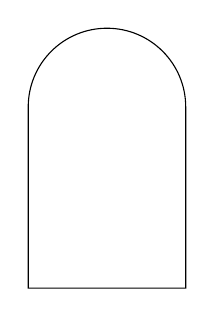
\begin{tikzpicture}
        \draw (0,0) -- (2,0) -- (2,2.3) arc (0:180:1) -- cycle;
    \end{tikzpicture}
\end{center}
\item 已知函数$f(x)=\sqrt{ax^2+x+1}$.\\
(1) 若函数$y=f(x)$的定义域为$(-\infty ,+\infty)$, 求实数$a$的取值范围;\\
(2) 若函数$y=f(x)$的值域为$[0,+\infty)$, 求实数$a$的取值范围.
\item 已知函数$f(x)=\sqrt x$, 函数$g(x)=\sqrt{1-x}-\sqrt x$, 则函数$y=f(x)+g(x)$的定义域为\blank{50}.
\item 已知函数$y=f(x)$的定义域为$[1,4]$, 则函数$y=\dfrac{f(2x)}{x-2}$的定义域是\blank{50}.
\item (1)设函数$D(x)=\begin{cases} 1, & x\in \mathbf{Q}, \\  0, &x\notin\mathbf{Q}. \end{cases}$ 令$F(x)=D(\sqrt 2x)$, 则$F(1)=$\blank{50};\\
(2) 已知函数$f(x)=\begin{cases} 2-x, & x<-2, \\ x^2, & -2\le x<1, \\ x, & x\ge 1. \end{cases}$ 若$f(x)=2$, 则$x$=\blank{50}.
\item 已知$f(x)=\begin{cases} x-2, & x>8, \\ f(x+3), & x\le 8, \end{cases}$ 则$f(2)=$\blank{50}.
\item 设常数$a\in \mathbf{R}$, $f(x)=\begin{cases}x+a, &x<a, \\ \dfrac 1x+a, & x\ge a. \end{cases}$ 若$f(2)=2$, 则$a=$\blank{50}.
\item 已知函数$f(x)=\begin{cases} \sqrt x, & x>1, \\ x, &x\le 1,  \end{cases}$ 函数$g(x)=1-\sqrt x$. 求函数$y=f(x)+g(x)$的解析式及定义域.
\item *设$D$是含数$1$的有限实数集, $f(x)$是定义在$D$上的函数, 若$f(x)$的图像绕原点逆时针旋转$\dfrac \pi6$后与原图像重合, 则在以下各项中, $f(1)$的可能取值只能是\bracket{20}
\fourch{$\sqrt3$}{$\dfrac{\sqrt{3}}2$}{$\dfrac{\sqrt{3}}3$}{$0$}
\item 设常数$p\in \mathbf{R}$, 设函数$f(x)=\log_2\dfrac{x+1}{x-1}+\log_2(x-1)+\log_2(p-x)$.\\
(1) 求$p$的取值范围以及函数$y=f(x)$的定义域;\\
(2) 若$y=f(x)$存在最大值, 求$p$的取值范围, 并求出最大值.
\item 已知$xy<0$, 且$4x^2-9y^2=36$. 问: 能否由此条件将$y$表示成$x$的函数? 若能, 求出该函数的解析式; 若不能, 说明理由.
\item 已知常数$a\in \mathbf{R}$, 函数$g(x)=\dfrac x{x+2}$, 函数$h(x)=\dfrac 1{x+a}$. 设函数$F(x)=g(x)\cdot h(x)$, $D_F$是其定义域; $f(x)=g(x)-h(x)$, $D_f$是其定义域.\\
(1) 设$a=2$, 求函数$F(x)$的值域;\\
(2) 对于给定的常数$a$, 是否存在实数$t$, 使得$f(t)=0$成立? 若存在, 求出这样的所有$t$的值; 若不存在, 说明理由;\\
(3) *是否存在常数$a$的值, 使得对于任意$x\in {D_f}\cap \mathbf{R}^+$, 有$f(x)\ge 0$恒成立? 若存在, 求出所有这样的a的值; 若不存在, 说明理由.

% 第九讲 8+3+10
\item 给定六个函数: \textcircled{1} $y=\dfrac 1x$; \textcircled{2} $y=x^2+1$; \textcircled{3} $y={x^{-\frac 13}}$; \textcircled{4} $y=2^x$; \textcircled{5} $y=\log_2x$; \textcircled{6} $y=\sqrt{x^2-1}+\sqrt{1-x^2}$.\\
在这六个函数中, 是奇函数但不是偶函数的是\blank{50}, 是偶函数但不是奇函数的是\blank{50}, 既不是奇函数也不是偶函数的是\blank{50}, 既是奇函数又是偶函数的是\blank{50}.
\item 设常数$a$、$b\in \mathbf{R}$. 若定义在$[a-2,2a]$上的$f(x)=ax^2+bx$是偶函数, 则$a=$\blank{50}, $b=$\blank{50}.
\item 设常数$a$、$b\in \mathbf{R}$. 若定义在$[a-1,a+1]$上的$f(x)=ax^2+x+b$是奇函数, 则$a=$\blank{50}, $b=$\blank{50}.
\item 若函数$f(x)=\dfrac{(x+1)(x+a)}x$为奇函数, 则实数$f(x)$\blank{50}.
\item 设函数$y=f(x)$为定义在$\mathbf{R}$上的函数, 则命题: ``$f(-1)\ne f(1)$且$f(-1)\ne -f(1)$''是命题``$y=f(x)$既不是奇函数也不是偶函数''的\blank{50}条件(填``充分不必要''、``必要不充分''、``充要''、``既不充分也不必要''之中一个).
\item 设$y=f(x)$是定义在$\mathbf{R}$上的函数, 当$x\ge 0$时, $f(x)=x^2-2x$.\\
(1) 当$y=f(x)$为奇函数时, 则当$x<0$时, $f(x)$=\blank{50};\\
(2) 当$y=f(x)$为偶函数时, 则当$x<0$时, $f(x)$=\blank{50}.
\item 设奇函数$y=f(x)$的定义域为$[-5, 5]$.若当$x\in [0,5]$时, $y=f(x)$的图像如图, 则不等式$xf(x)<0$的解是\blank{50}.
\begin{center}
    \begin{tikzpicture}[>=stealth]
        \draw [->] (-1,0) -- (6,0) node [below] {$x$};
        \draw [->] (0,-2.5) -- (0,2.5) node [left] {$y$};
        \draw (2,0) node [below] {$2$};
        \draw (5,0) node [above] {$5$};
        \draw [domain = 0:2,samples = 100] plot (\x,-\x*\x+2*\x);
        \draw [domain = 2:5,samples = 100] plot (\x, \x*\x/2-4*\x+6);
        \draw [dashed] (5,0) -- (5,-1.5);
        \draw (0,0) node [below left] {$O$};
    \end{tikzpicture}
\end{center}
\item 若定义在$\mathbf{R}$上的两个函数$y=f(x)$、$y=g(x)$均为奇函数. 设$F(x)=af(x)+bg(x)+1$.\\
(1) 若$F(-2)=10$, 则$F(2)=$\blank{50};\\
(2) 若函数$y=F(x)$在$(0,+\infty)$上存在最大值$4$, 则$y=F(x)$在$(-\infty ,0)$上的最小值为\blank{50}.
\item 判断下列函数$y=f(x)$的奇偶性:\\
(1) $f(x)=(x-1)\cdot \sqrt{\dfrac{1+x}{1-x}}$;\\
(2)$f(x)=\begin{cases} x(1-x), & x<0, \\ x(1+x),& x>0. \end{cases}$.
\item 已知函数$f(x)=x^2-2a|x-1|$, $x\in \mathbf{R}$, 常数$a\in \mathbf{R}$.\\
(1) 求证: 函数$y=f(x)$不是奇函数;\\
(2) 若函数$y=f(x)$是偶函数, 求实数$f(x)=\log_3| 2x+a |$的值.
\item 判断下列函数$y=f(x)$的奇偶性:\\
(1) $f(x)=\dfrac 1{a^x-1}+\dfrac 12$(常数$a>0$且$a\ne 1$);\\
(2) $f(x)=\dfrac{ax}{x^2-a}$(常数$a\in \mathbf{R}$).
\item 设$y=f(x)$是定义在$\mathbf{R}$上的函数, 则下列叙述正确的是\bracket{20} .
\twoch{$y=f(x)f(-x)$是奇函数}{$y=f(x)|f(-x)|$是奇函数}{$y=f(x)-f(-x)$是偶函数	}{$y=f(x)+f(-x)$是偶函数}
\item 设函数$y=f(x)$为定义在$\mathbf{R}$上的函数, 则``$f(0)\ne 0$''是``函数$y=f(x)$不是奇函数''的\bracket{20}.
\twoch{充分非必要条件}{必要非充分条件}{充要条件}{既不是充分条件, 也不是必要条件}
\item 设$y=f(x)$是定义在$\mathbf{R}$上的奇函数, 当$x<0$时, $f(x)=\lg(2-x)$, 则$x\in \mathbf{R}$时, $f(x)$=\blank{50}.
\item 判断下列函数$y=f(x)$的奇偶性, 并说明理由:\\
(1) $f(x)=x^3-\dfrac 1x$;\\
(2) $f(x)=\dfrac{|x+3|-3}{\sqrt{4-x^2}}$.
\item 根据常数$a$的不同取值, 讨论下列函数$y=f(x)$的奇偶性, 并说明理由:\\
(1) $f(a)\ge f(0)$;\\
(2) $f(x)=x|x-a|$.
\item 设函数$y=f(x)$是定义在$\mathbf{R}$上的奇函数. 若$x>0$时, $f(x)=\lg x$.\\
(1) 求方程$f(x)=0$的解集;\\
(2) 求不等式$f(x)>-1$的解集.
\item 是否存在实数$b$, 使得函数$g(x)=\dfrac{2^x}{{4^x}-b}$是奇函数? 若存在, 求$b$的值; 若不存在, 说明理由.
\item 常数$a\in \mathbf{R}$. 若函数$f(x)=\lg(10^x+1)+ax$是偶函数, 则$a=$\blank{50}.
\item 已知$y=f(x)$为定义在$\mathbf{R}$上的奇函数, $y=g(x)$为定义在$\mathbf{R}$上的偶函数, 且任意$x\in \mathbf{R}$, 都有$f(x)=g(x)+\dfrac{1}{x^2+x+1}$, 则$f(1)+g(1)=$\blank{50}.
\item 设常数$a\ne 0$. 若函数$f(x)=\lg \dfrac{x+1-2a}{x+1+3a}$. 是否存在实数$a$, 使函数$y=f(x)$为奇函数或偶函数? 若存在, 求出$a$的值, 并判断相应的$y=f(x)$的奇偶性; 若不存在, 说明理由.

%第十讲 9+2+10
\item 函数$y=\dfrac 1{x^2-4x+5}$的图像关于\bracket{20}.
\fourch{$y$轴对称}{原点对称}{直线$x=2$对称}{点$(2,1)$对称}
\item 函数$y=x+\dfrac 1{x-1}$的图像关于\bracket{20}.
\fourch{点$(1,1)$对称}{点$(-1,1)$对称}{点$(1,-1)$对称}{点$(-1,-1)$对称}
\item 若函数$y=f(x)$的定义域为$\mathbf{R}$, 且$f(x-1)=-f(3-x)$, 则$y=f(x)$的图像关于\bracket{20}.
\fourch{原点中心对称}{点$(1,0)$中心对称}{点$(2,0)$中心对称}{点$(4,0)$中心对称}
\item 设常数$a,b\in \mathbf{R}$.若函数$y=x^2+ax$在区间$[a,b]$上的图像关于直线$x=1$对称, 则$b=$\blank{50}.
\item 已知函数$y=f(x)$满足: 对于任意$x\in \mathbf{R}$, 都有$f(x+1)=-f(x)$. 若$f(1)=1$, 则$f(4)=$\blank{50}; $f(2015)=$\blank{50}.
\item 已知函数$y=f(x)$图像关于$(1,0)$对称. 若$x\le 1$时, $f(x)=x^2-1$, 则$f(x)=$\blank{50}.
\item 已知函数$y=f(x)$满足: 对于任意$x\in \mathbf{R}$, 都有$f(x+3)=f(x)$. 若$x\in [0,3)$时, $f(x)=x-1$, 则$x\in [6,9)$时, $f(x)=$\blank{50}.
\item 设常数$a\in \mathbf{R}$.已知函数$y=f(x)$满足: 对于任意$x\in \mathbf{R}$, 都有$f(x-1)=f(1-x)$. 若函数$y=f(x)$图像总是关于直线$x=a$对称, 则$a$=\blank{50}.
\item 设常数$a\in \mathbf{R}$.若直线$x=2$是函数$f(x)=\log_3|2x+a|$的图像的一条对称轴, 则$a$=\blank{50}.
\item 设函数$y=f(x)$为$\mathbf{R}$上的奇函数, 且对于任意$x\in \mathbf{R}$都有$f(x+2)=-f(x)$.\\
(1) 求证: 函数$y=f(x)$为周期函数;\\
(2) 对于任意$x\in \mathbf{R}$, 求证: $f(1+x)=f(1-x)$;\\
(3) 设$0\le x\le 1$时, $f(x)=\dfrac 12x$. 求函数$y=f(x)+\dfrac 12$在$-4\le x\le 4$时的所有零点;\\
(4) 设$-1\le x\le 1$时, $f(x)=\sin x$.\\
\textcircled{1} 写出$1\le x\le 5$时, $y=f(x)$的解析式;\\
\textcircled{2} 求$y=f(x)$在$\mathbf{R}$上的解析式.
\item 常数$a$、$b\in \mathbf{R}$. 函数$f(x)=\dfrac x{\sqrt 3}+\dfrac 1{x+a}+b$的图像关于点$(1,2)$对称.\\
(1) 求$y=f(x)$的解析式;\\
(2) *若$y=f(x)$的图像关于某一条直线对称, 写出这样的一条对称轴直线的方程(无需证明).
\item 函数$y=\log_2\dfrac{2-x}{2+x}$的图像关于\bracket{20}.
\fourch{原点对称}{$y$轴对称}{直线$y=x$对称}{直线$y=-x$对称}
\item 函数$y=\log_2(2-2^x)$的图像关于\bracket{20}.
\fourch{原点对称}{$y$轴对称}{直线$y=x$对称}{直线$y=-x$对称}
\item 设常数$a$、$b\in \mathbf{R}$. 若二次函数$f(x)=ax^2+bx+1$满足: 对任意$t\in \mathbf{R}$, $f(2+t)=f(2-t)$, 则$\dfrac ba=$\blank{50}.
\item 设定义在$\mathbf{R}$上的函数$y=f(x)$的图像关于直线$x=1$对称. 若$x\ge 1$时, $f(x)=1-3^{x-1}$, 则$x<1$时, $f(x)=$\blank{50}.
\item 设函数$y=\log_2(x+3)$的图像与函数$y=f(x)$的图像关于直线$x=1$对称. \textcircled{1} $f(1)$=\blank{50}; \textcircled{2} 若$f(a)$有意义, 则$f(a)=$\blank{50}(结果用$a$的表达式表示).
\item 已知定义域为$\mathbf{R}$的函数$y=f(x)$是偶函数, 并且其图像关于直线$x=1$对称.\\
(1) 若$f(0)=1$, $f(1)=2$, 求$f(15)+2f(20)$的值;\\
(2) 设$x\in [0,1]$时, $f(x)=x^3$.\\
\textcircled{1} $1<x\le 2$时, 求$y=f(x)$的解析式;\\
\textcircled{2} $-2\le x<0$时, 求$y=f(x)$的解析式;\\
\textcircled{3} 求函数$y=f(x)-\dfrac 18$在$[-2,2]$上的所有零点;\\
\textcircled{4} 求$y=f(x)$在$\mathbf{R}$上的解析式.
\item 已知$f(x)$是定义域为$(-\infty,+\infty)$的奇函数, 满足$f(1-x)=f(1+x)$. 若$f(1)=2$, 则$f(1)+f(2)+f(3)+\cdots +f(50)=$\bracket{20}.
\fourch{$-50$}{$0$}{$2$}{$50$}
\item 已知函数$y=f(x)$对一切$u,v\in \mathbf{R}$, 都有$f(u+v)=f(u)+f(v)$.\\
(1)	求证: $y=f(x)$是奇函数;\\ 
(2) 若$f(-3)=a$, 用$a$表示$f(6)$以及$f(300)$.
\item 已知定义在$\mathbf{R}$上的函数$y=f(x)$是奇函数, 且$y=f(x)$也是以4为周期的一个周期函数.\\
(1) 若$f(1)=1$, 则$f(-1)+f(0)=$\blank{50}; $f(10)+f(11)=$\blank{50};\\
(2) *若$f(1)=0$, 则在区间$[-3,3]$上的零点的个数的最小值为\blank{50}.
\item *设定义在$\mathbf{R}$上的函数$y=f(x)$的满足: 对于任意$x\in \mathbf{R}$, 恒有$f(-x+1)=-f(x+1)$且$f(-x-1)=-f(x-1)$. 则下面命题中, 正确的命题的序号是\blank{50}.\\
\textcircled{1} 函数$y=f(x)$是偶函数; \textcircled{2} $2$是$y=f(x)$的周期; \textcircled{3} 函数$y=f(x)$图像关于$(1,0)$对称; \textcircled{4} 函数$y=f(x)$图像关于$(3,0)$对称.


% 第十一讲 10+3+10
\item 下列函数中, 在其定义域上是单调函数的序号为\blank{50}.\\
\textcircled{1} $y=\dfrac{2-x}x$; \textcircled{2} $y=x-\dfrac 1x$; \textcircled{3} $y={3^{x-1}}$; \textcircled{4} $y=ln\dfrac 1x$; \textcircled{5} $y=tanx$.
\item 函数$y=|x-1|$递减区间的是\blank{50}.
\item 函数$y=x+\dfrac 2x$($x>0$)的递减区间是\blank{50}.
\item 函数$y=(\dfrac 12)^{x^2}$的递减区间是\blank{50}.
\item 函数$y=\dfrac 1{\sqrt{x^2+2x-3}}$的递增区间是\blank{50}.
\item 设常数$a\in \mathbf{R}$.若$y=\dfrac{ax}{x+1}$在区间$(-1,+\infty)$上递增, 则$a$的取值范围是\blank{50}.
\item 设常数$a\in \mathbf{R}$.若函数$y=x^2+ax+1$在$(-\infty,2]$上递减, 则$a$的取值范围是\blank{50}.
\item 若函数$y=f(x)$, $y=g(x)$均为$\mathbf{R}$上增函数, 则下列命题中, 正确的命题的序号是\blank{50}.\\
\textcircled{1} $y=f(x)+g(x)$为增函数; \textcircled{2} $y=f(x)\cdot g(x)$为增函数; \textcircled{3} $y=f(g(x))$为增函数.
\item 若$y=f(x)$为$\mathbf{R}$上的奇函数, 且在$(-\infty,0)$上是减函数, 又$f(-2)=0$, 则$f(x)\le 0$的解集为\blank{50}.
\item 设常数$a\in \mathbf{R}$. 若函数$f(x)=\begin{cases} x+a,& x<1, \\ x^2,& x\ge 1 \end{cases}$在$\mathbf{R}$上递增, 则$a$的取值范围为\blank{50}.
\item 设函数$f(x)=\mathrm{e}^x+\dfrac 1{\mathrm{e}^x}$.\\
(1) 求证: $y=f(x)$在$\mathbf{R}$上不是增函数;\\
(2) 求证: $y=f(x)$在$[0,+\infty)$上是增函数.
\item 设常数$a\in \mathbf{R}$. 若$y=\log_{\frac 12}(x^2-ax+2)$在$[-1,+\infty)$上是减函数, 求$a$的取值范围.
\item 已知定义在区间$(-1,1)$上的函数$y=f(x)$是奇函数, 也是减函数. 若$f(1-a)+f(1-a^2)<0$, 求实数$a$的取值范围.
\item 下列函数中, 在区间$(0 ,+\infty)$上递增的函数的序号为\blank{50}.\\
\textcircled{1} $y=|x+1|$;  \textcircled{2} $y=x-\dfrac 1x$;    \textcircled{3} $y={x^{\frac 12}}$;    \textcircled{4} $y=\sqrt{1-\dfrac 1x}$; \textcircled{5} $y=\lg x$.
\item 函数$y=\log_{0.7}(x^2-3x+2)$的单调减区间为\blank{50}.
\item 已知$y=f(x)$是偶函数, 且在区间$[0,4]$上递减. 记$a=f(2)$, $b=f(-3)$, $c=f(-4)$, 则将$a,b,c$按从小到大的顺序排列是	\blank{50}.	
\item 设常数$a\in \mathbf{R}$. ``$a=1$''是``$f(x)=|x-a|$在区间$[1, +\infty)$上为增函数''的\blank{50}条件(填: ``充分不必要''、``必要不充分''、``充要''、``既不充分也不必要''之一).
\item (1) 设常数$a\in \mathbf{R}$.若函数$y=\dfrac 1{x-a}$在区间$(0,+\infty)$上单调, 则$a$的取值范围为\blank{50}.\\
(2) 设常数$k\in \mathbf{R}$.若函数$f(x)=kx^2-4x+8$在区间$[5,20]$上单调递减, 则$k$的取值范围是\blank{50}.
\item  *设$f(x)$、$g(x)$、$h(x)$是定义域为$R$的三个函数, 对于下列命题:\\
\textcircled{1} 若$f(x)+g(x)$、$f(x)+h(x)$、$g(x)+h(x)$均为增函数, 则$f(x)$、$g(x)$、$h(x)$中至少有一个是增函数;\\
\textcircled{2} 若$f(x)+g(x)$、$f(x)+h(x)$、$g(x)+h(x)$均是以$T$为周期的函数, 则$f(x)$、$g(x)$、$h(x)$均是以$T$为周期的函数, 下列判断正确的是\bracket{20}.
\twoch{\textcircled{1}和\textcircled{2}均为真命题}{\textcircled{1}和\textcircled{2}均为假命题}{\textcircled{1}为真命题, \textcircled{2}为假命题}{\textcircled{1}为假命题, \textcircled{2}为真命题}
\item 设常数$a,b\in \mathbf{R}$. 已知$f(x)=\dfrac{ax^2+1}{x+b}$是奇函数, $f(1)=5$.\\
(1) 求$a,b$的值;\\
(2) 求证: $y=f(x)$在区间$(0,\dfrac 12]$上是减函数.
\item 求证: 函数$f(x)=\dfrac 1x-\lg\dfrac{1+x}{1-x}$是奇函数, 且在区间$(0,1)$上递减.
\item 设常数$a\in \mathbf{R}$.若函数$f(x)=\log_a(2-ax)$在$[0,1]$上是减函数, 求$a$的取值范围.
\item 已知定义$\mathbf{R}$上的函数$y=f(x)$满足下面两个条件:\\
(I) 对于任意$x_1,x_2\in \mathbf{R}$, 都有$f(x_1+x_2)=f(x_1)+f(x_2)$; (II)当$x>0$时, $f(x)>0$, 且$f(1)=1$.\\
(1) 求证: $y=f(x)$是奇函数;\\
(2) 求证: $y=f(x)$在$\mathbf{R}$上是增函数;\\
(3) *解不等式$f(x^2-1)<2$.

% 第十二讲 10+3+10
\item 函数$y=x^{-\frac 32}$的定义域为\blank{50}.
\item 下列命题中, 正确的命题的序号是\blank{50}.\\
\textcircled{1} 当$\alpha =0$时, 函数$y={x^{\alpha }}$的图像是一条直线;\\
\textcircled{2} 幂函数的图像都经过(0, 0)和(1, 1)点;\\
\textcircled{3} 当$\alpha <0$且$y={x^{\alpha }}$是奇函数时, 它也是减函数;\\
\textcircled{4} 第四象限不可能有幂函数的图像.
\item 图中曲线是幂函数$y=x^n$在第一象限的图像, 已知$n$取$\pm 2$, $\pm\dfrac 12$四个值, 则相应于曲线$c_1,c_2,c_3,c_4$的$n$依次为\bracket{20}.
\begin{center}
    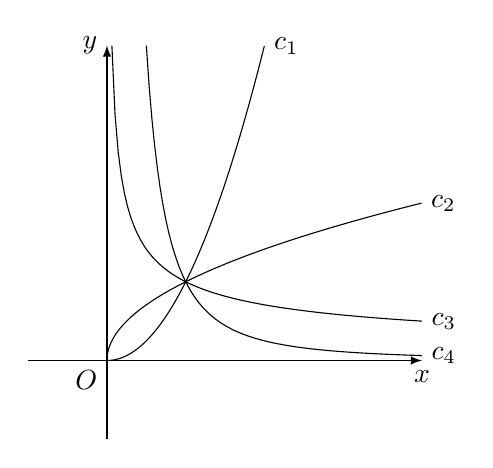
\begin{tikzpicture}[>=latex]
        \draw [->] (-1,0) -- (4,0) node [below] {$x$};
        \draw [->] (0,-1) -- (0,4) node [left] {$y$};
        \draw (0,0) node [below left] {$O$};
        \draw [domain = 0:2, samples = 100] plot (\x,\x*\x) node [right] {$c_1$};
        \draw [domain = 0:2, samples = 100] plot (\x*\x,\x) node [right] {$c_2$};
        \draw [domain = 0.0625:4, samples = 100] plot (\x, {1/sqrt(\x)}) node [right] {$c_3$};
        \draw [domain = 0.5:4, samples = 100] plot (\x, {1/\x/\x}) node [right] {$c_4$};
    \end{tikzpicture}
    \end{center}
\fourch{$-2,-\dfrac 12,\dfrac 12,2$}{$2,\dfrac 12,-\dfrac 12,-2$
}{$-\dfrac 12,-2,2,\dfrac 12$}{$2,\dfrac 12,-2,-\dfrac 12$}
\item 下列函数的图像为(A)、(B)、(C)、(D)之一, 试将正确的字母标号填在相应函数后面的横线上.
\begin{center}
    \begin{tikzpicture}[>=latex,scale = 0.5]
        \draw [->] (-3,0) -- (3,0) node [below] {$x$};
        \draw [->] (0,-3) -- (0,3) node [left] {$y$};
        \draw (0,0) node [below right] {$O$};
        \draw [domain = {-3^(1/4)}:{3^(1/4)}] plot (\x*\x*\x,\x*\x*\x*\x);
        \draw (0,-3) node [below] {(A)};
    \end{tikzpicture}
    \begin{tikzpicture}[>=latex,scale = 0.5]
        \draw [->] (-3,0) -- (3,0) node [below] {$x$};
        \draw [->] (0,-3) -- (0,3) node [left] {$y$};
        \draw (0,0) node [below right] {$O$};
        \draw [domain = {-3^(1/5)}:{3^(1/5)}] plot (\x*\x*\x,\x*\x*\x*\x*\x);
        \draw (0,-3) node [below] {(B)};
    \end{tikzpicture}
    \begin{tikzpicture}[>=latex,scale =0.5]
        \draw [->] (-3,0) -- (3,0) node [below] {$x$};
        \draw [->] (0,-3) -- (0,3) node [left] {$y$};
        \draw (0,0) node [below right] {$O$};
        \draw [domain = {0}:{3^(1/3)}] plot (\x*\x,\x*\x*\x);
        \draw (0,-3) node [below] {(C)};
    \end{tikzpicture}
    \begin{tikzpicture}[>=latex,scale = 0.5]
        \draw [->] (-3,0) -- (3,0) node [below] {$x$};
        \draw [->] (0,-3) -- (0,3) node [left] {$y$};
        \draw (0,0) node [below right] {$O$};
        \draw [domain = {3^(-3/2)}:3] plot (\x,{\x^(-2/3)}) plot (-\x,{\x^(-2/3)});
        \draw (0,-3) node [below] {(D)};
    \end{tikzpicture}
    \end{center}
(1) $y=x^\frac 32$\blank{50}; (2) $y=x^\frac 43$\blank{50}; (3) $y=x^\frac 53$\blank{50}; (4) $y=x^{-\frac 23}$\blank{50}.
\item 已知$\alpha\in \{-2,-1,-\dfrac 12,\dfrac 12,1,2,3\}$, 若幂函数$f(x)=x^\alpha$为奇函数, 且在$(0,+\infty)$上递减, 则$\alpha=$\blank{50}.
\item 函数$y=f(x)$满足两个条件:
\textcircled{1} $y=f(x)$是两个幂函数的和函数; \textcircled{2} $y=f(x)$的最小值为2, 则$y=f(x)$的解析式可以是\blank{50}.
\item 若集合$A=\{y|y={x^{\frac 13}}, \ -1\le x\le 1\}$, $B=\{y|y={x^{-\frac 12}}\}$, 则$A\cap B$等于\bracket{20}.
\fourch{$(0,1]$}{$[-1,1]$}{$\{1\}$}{$\{0,1\}$}
\item 设常数$m\in \mathbf{R}$. 若幂函数$y=(m^2-m-1)x^{m^2-2m-1}$在$(0,+\infty)$上是增函数, 则$m$的值为\blank{50}.
\item 设常数$n\in \mathbf{Z}$. 若函数$y=x^{n^2-2n-3}$的图像与两条坐标轴都无公共点, 且图像关于$y$轴对称, 则$n$的值为\blank{50}.
\item 函数$y=1-(x+2)^{-2}$可以先将幂函数$y=x^{-2}$的图像向\blank{50}平移$2$个单位, 再以\blank{50}轴为对称轴作对称变换, 最后向\blank{50}平移$1$个单位.
\item 在$f(x)=(2m^2-7m-9)x^{m^2-9m+19}$中, 当实数$m$为何值时,\\
(1) $y=f(x)$是正比例函数, 且它的图像的倾斜角为钝角?\\
(2) $y=f(x)$是反比例函数, 且它的图像在第一, 三象限?
\item 设常数$t\in \mathbf{Z}$. 已知幂函数$y=(t^3-t+1){x^{\frac 13(1+2t-t^2)}}$是偶函数, 且在区间$(0,+\infty)$上是增函数, 求整数$t$的值, 并作出相应的幂函数的大致图像.
\item 设$a\in \mathbf{R}$.\\
(1) 若$(a+2)^{\frac 23}>{(1-2a)}^{\frac 23}$, 求$a$的取值范围;\\
(2) 若$(a+2)^{-\frac 13}>(1-2a)^{-\frac 13}$, 求$a$的取值范围.
\item 已知函数: \textcircled{1} $y=\dfrac 1x$; \textcircled{2} $y=x^{\dfrac 12}$; \textcircled{3} $y=x^{-\dfrac 12}$; \textcircled{4} $y={x^{\dfrac 23}}$; \textcircled{5} $y=x^{-\dfrac 23}$, 填写分别具有下列性质的函数序号:\\ 
(1) 图像与$x$轴有公共点的:\blank{50};\\
(2) 图像关于原点对称的:\blank{50};\\
(3) 定义域内递减的:\blank{50};\\
(4) 在定义域内有反函数的:\blank{50}.
\item 函数$y=-(x+1)^{-3}$的图像可以先将幂函数$y=x^{-3}$的图像向\blank{50}平移1个单位, 再以\blank{50}轴为对称轴作对称变换.
\item 设$\alpha \in \{-3,-\dfrac 23,-\dfrac 12,-\dfrac 13,\dfrac 13,1,\dfrac 32,2\}$. 已知幂函数$y=x^{\alpha}$是奇函数, 且在区间$(0,+\infty)$上是减函数, 则满足条件的$\alpha$的值是\blank{50}.
\item 下列关于幂函数图像及性质的叙述中, 正确的叙述的序号是\blank{50}.\\
\textcircled{1} 对于一个确定的幂函数, 第二、三象限不可能同时有该幂函数的图像上的点;\\
\textcircled{2} 若某个幂函数图像过$(-1,-1)$, 则该幂函数是奇函数;\\
\textcircled{3} 若某个幂函数在定义域上递增, 则该幂函数图像必经过原点;\\
\textcircled{4} 幂函数图像不会经过点$(-\dfrac 12,8)$以及$(-8,-4)$.
\item 设$y=f(x)$与$y=g(x)$是两个不同的幂函数, 集合$M=\{x|f(x)=g(x)  \}$, 则集合$M$中的元素是\bracket{20}.
\fourch{$1$或$2$}{$1$或$3$}{$1$或$2$或$3$}{$1$或$2$或$3$或$4$}
\item 已知幂函数$y=x^{\frac qp}$($p\in \mathbf{N}^*,\ q\in \mathbf{N}^*$, $p,q$互质)的图像如图所示, 则\bracket{20}.
\begin{center}
    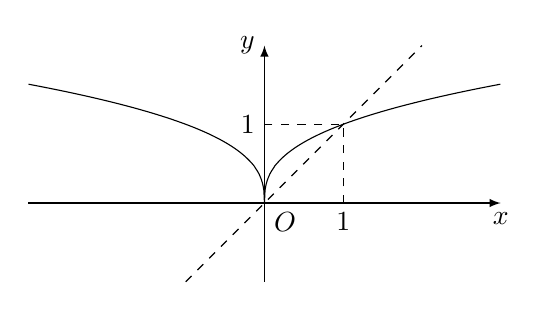
\begin{tikzpicture}[>=latex]
        \draw [->] (-3,0) -- (3,0) node [below] {$x$};
        \draw [->] (0,-1) -- (0,2) node [left] {$y$};
        \draw (0,0) node [below right] {$O$};
        \draw [dashed] (-1,-1) -- (2,2);
        \draw [domain = 0:3, samples = 400] plot (\x,{\x^(3/8)}) plot (-\x,{\x^(3/8)});
        \draw [dashed] (1,0) node [below] {$1$} -- (1,1) -- (0,1) node [left] {$1$};
    \end{tikzpicture}
\end{center}
\twoch{$p,q$均为奇数}{$p$是奇数, $q$是偶数, 且$0<\dfrac qp<1$}{$p$是偶数, $q$是奇数}{$p$是奇数, $q$是偶数, 且$\dfrac qp>1$}
\item 若$(x+1)^{-\frac 13}<(3-2x)^{-\frac 13}$, 求实数$x$的取值范围.
\item 设常数$a,b$满足$a>b>0$. 已知函数$f(x)=\dfrac{x+a}{x+b}$.
(1) 写出函数$y=f(x)$的单调性;\\
(2) 写出函数$y=f(x)$图像的一个对称中心的坐标.
\item 已知函数$f(x)=\dfrac{x^{\frac 13}-x^{-\frac 13}}5$, $g(x)=\dfrac{x^{\frac 13}+x^{-\frac 13}}5$.\\
(1) 分别计算$f(4)-5f(2)g(2)$和$f(9)-5f(3)g(3)$的值;\\
(2) 由(1)概括出涉及函数$y=f(x)$和$y=g(x)$的, 对所有不等于零的实数$x$都成立的一个等式, 并加以证明.
\item *设常数$a,b$满足$a>b>0$. 已知函数$f(x)=\dfrac{x+a}{x+b}$. 证明: 该函数图像的对称中心是唯一的.

% 第十二讲 9+2+9

\item 函数$y=\log_2 \dfrac 1{x-1}$的反函数是\blank{50}.
\item 函数$y=x^2$($x\le 0$)的反函数是\blank{50}.
\item 函数$y=\dfrac{2^x}{{2^x}-1}$($x>0$)的反函数是\blank{50}.
\item 已知函数$y=f(x)$的反函数是$f^{-1}(x)=\dfrac{4x+3}{2x-1}$, 则$f(x)$=\blank{50}.
\item 记$y=f^{-1}(x)$是$y=f(x)$的反函数. 若函数$f(x)=\log_3x$, 则$f^{-1}(-\log_9 2)$=\blank{50}.
\item 若命题``函数$y=x+\dfrac ax$在区间$[1,2]$上存在反函数''为真命题, 则在下列值中, 能作为实数$a$的值的序号是\blank{50}.\\
\textcircled{1} $a=-1$; \textcircled{2} $a=1$; \textcircled{3} $a=\sqrt 2$; \textcircled{4} $a=\sqrt 5$.
\item 若函数$f(x)=1-\sqrt{1-x^2}\ (-1\le x\le 0)$,
请画出函数$y={f^{-1}}(x)$的大致图像.
\begin{center}
    \begin{tikzpicture}[>=latex,scale =1.8]
        \foreach \i in {-1,-0.5,0,0.5,1} {\draw [dashed, gray!90] (\i,-1) -- (\i,1) (-1,\i) -- (1,\i);};
        \draw [->] (-1.5,0) -- (1.5,0) node [below] {$x$};
        \draw [->] (0,-1.5) -- (0,1.5) node [left] {$y$};
        \draw (0,0) node [below left] {$O$};
        \draw (1,0) node [below] {$1$} (0,1) node [left] {$1$};
    \end{tikzpicture}
\end{center}
\item 已知定义在$\mathbf{R}$上的函数$y=f(x)$是奇函数, 且有反函数$y=f^{-1}(x)$. 若$a,b$是两个实数, 则下列点中, 必在$y=f^{-1}(x)$的图像上的点的序号是\blank{50}.\\
\textcircled{1} $(-f(a),a)$; \textcircled{2} $(-f(a),-a)$;\textcircled{3} $(-b,-f(b))$; \textcircled{4} $(b,-f^{-1}(-b))$.
\item 已知定义在$\mathbf{R}$上的函数$y=f(x)$的反函数为$y=f^{-1}(x)$.若$y=f(x+1)$的图像过点$(-\dfrac 12,1)$, 则$y=f^{-1}(x+1)$的图像必过\bracket{20}.
\fourch{$(1,-\dfrac 12)$}{$(1,\dfrac 12)$}{$(0,-\dfrac 12)$}{$(0,\dfrac 12)$}
\item 设常数$a\ne 0$. 若函数$f(x)=\dfrac{1-ax}{1+ax}$的图像关于直线$y=x$对称, 求实数$a$的值以及$y=f(x)$的反函数$y=f^{-1}(x)$.
\item 记$y=f^{-1}(x)$是$y=f(x)$的反函数.\\
(1) 若函数$f(x+1)=\dfrac x{x+1}$, 求函数$y=f^{-1}(x+1)$的解析式;\\
(2) 设函数$f(x)=\dfrac{1-2x}{1+x}$. 若$y=g(x)$的图像与$y=f^{-1}(x+1)$的图像关于直线$y=x$对称, 求$y=g(x)$的解析式.
\item (1) 函数$y=x^2+2x-3\ (x\ge 0)$的反函数为\blank{50};\\
(2) 函数$y=\dfrac{\mathrm{e}^x-1}{{\mathrm{e}}^x+1}$的反函数为\blank{50};\\
(3) 函数$y=x|x|$的反函数为\blank{50}.
\item 已知函数$y=f(x)$是奇函数, 且$y=g(x)$是$y=f(x)$的反函数. 若$x\ge 0$时, $f(x)=3^x-1$, 则$g(-8)$=\blank{50}.
\item 设常数$a\in \mathbf{R}$. 若函数$y=x+\dfrac ax$在区间$[1,2]$上存在反函数, 求$a$的取值范围.
\item 求函数$y=\begin{cases}x^2-2x+2, & x\le 1,\\(\dfrac 12)^x, & x>1  \end{cases}$的反函数.
\item 设常数$a>0$且$a\ne 1$. 求函数$f(x)=\log_a(x+\sqrt{x^2-1})$的反函数.
\item 已知函数$y=f(x)$的图像经过点$(0,-1)$. 若函数$y=f(x+4)$存在反函数$y=g(x)$, 则$y=g(x)$的图像总经过的定点的坐标为\blank{50}.
\item 设$y=f^{-1}(x)$, $y=g^{-1}(x)$分别是定义在$\mathbf{R}$上的函数$y=f(x)$, $y=g(x)$的反函数. 若函数$y=f(x-1)$和$y=g^{-1}(x-3)$的图像关于直线$y=x$对称, 且$g(5)=2018$, 则 $f(4)$的值为\blank{50}.
\item 设$a>0$, 函数$f(x)=\dfrac 1{1+a\cdot 2^x}$.\\
(1) 若$a=1$, 求$f(x)$的反函数$f^{-1}(x)$;\\
(2) 求函数$y=f(x)\cdot f(-x)$的最大值(用$a$表示);\\
(3) *设$g(x)=f(x)-f(x-1)$. 若对任意$x\in (-\infty ,0]$, $g(x)\ge g(0)$恒成立, 求$a$的取值范围.
\item 已知函数$y=f^{-1}(x)$是$y=f(x)$的反函数. 定义: 若对给定的实数$a(a\ne 0)$, 函数$y=f(x+a)$与$y=f^{-1}(x+a)$互为反函数, 则称$y=f(x)$满足``$a$和性质''.\\
(1) 判断函数$g(x)=x^2+1(x>0)$是否满足``$1$和性质'', 并说明理由;\\
(2) *求所有满足``$2$和性质''的一次函数. 

% 第十四讲 8+3+10
\item 若$\log_35=a$, $\log_57=b$ , 用$a,b$表示$\log_{75}63=$\blank{50}.
\item 若$3^a=4^b=6^c$, 且$a,b,c$都是正数, 则$\dfrac{-2ab+2bc+ac}{abc}$的值为\blank{50}.
\item 若不等式$(a-1)^x<1$的解集为$(-\infty,0)$, 则实数$a$的取值范围是\blank{50}.
\item 函数$f(x)=\dfrac{\sqrt{4-x^2}}{\lg |x-1|}$的定义域为\blank{50}.
\item 为了得到函数$y=\lg\dfrac{x+3}{10}$的图像, 只需把函数$y=\lg x$的图像上所有的点\bracket{20}.
\onech{向左平移$3$个单位长度, 再向上平移$1$个单位长度}{向右平移$3$个单位长度, 再向上平移$1$个单位长度}{向左平移$3$个单位长度, 再向下平移$1$个单位长度}{向右平移$3$个单位长度, 再向下平移$1$个单位长度}
\item 设常数$a>0,\ a\ne 1$. 函数$f(x)=a^x$在$[0,1]$上的最大值和最小值之和为$a^2$, 则$a=$\blank{50}.
\item 若集合$A=\{y|y=2\cdot (\dfrac 13)^{|x|}\}$, $B=\{ a|\log_a(3a-1)>0\}$, 则$A\cap B$=\blank{50}.
\item *已知函数$f(x)=|3^x-1|$, $c<b<a$, 且$f(b)<f(a)<f(c)$, 在下列关系式中, 一定成立的关系式的序号是\blank{50}.
\textcircled{1} $3^a+3^b>2$; \textcircled{2} $3^a+3^b<2$; \textcircled{3} $3^c<1$; \textcircled{4} $3^a+3^c<2$.
\item 已知函数$f(x)=\dfrac{3^x-3^{-x}}{3^x+3^{-x}}$.\\
(1) 证明$f(x)$在$(-\infty,+\infty)$上是增函数;\\
(2) 求$f(x)$的值域.
\item 已知函数$y=(\log_2\dfrac x{2^a})(\log_2\dfrac x4)$, $x\in [\sqrt 2,4]$, 试求该函数的最大值$g(a)$.
\item 已知函数$f(x)=a\cdot 2^x+b\cdot 3^x$, 其中常数$a,b$满足$ab\ne 0$.\\
(1) 若$ab>0$, 判断函数$y=f(x)$的单调性;\\
(2) 若$ab<0$, 求$f(x+1)>f(x)$时$x$的取值范围.
\item 不等式$\log_{\frac 12}(x-1)\ge 1$的解集为\blank{50}.
\item 设常数$a\in \mathbf{R}$. 若函数$f(x)=\dfrac 1{2^x-1}+a$为奇函数, 则$a$=\blank{50}.
\item 若$\log_23=a$, $3^b=7$, 用$a,b$表示$\log_{3\sqrt 7}2$, 则$\log_{3\sqrt 7}2$=\blank{50}.
\item 对于函数$y=f(x)$的定义域中的任意的$x_1,x_2$($x_1\ne x_2$), 有如下结论:\\
\textcircled{1} $f(x_1+x_2)=f(x_1)\cdot f(x_2)$; \textcircled{2} $f(x_1\cdot x_2)=f(x_1)+f(x_2)$;\\ \textcircled{3} $\dfrac{f(x_1)-f(x_2)}x_1-x_2>0$; \textcircled{4} $f(\dfrac{x_1+x_2}2)<\dfrac{f(x_1)+f(x_2)}2$. 
\\当$y=\ln x$时, 上述结论中, 正确结论的序号是\blank{50}.
\item (1) *函数$y=\log_a|x-b|$在$(0,+\infty)$上递增, 则$a$、$b$满足\bracket{20}.
\fourch{$a>1$且$b\ge 0$}{$a>1$且$b\le 0$}{$0<a<1$且$b\ge 0$}{$0<a<1$且$b\le 0$}
(2) 函数$f(x)=\log_a|ax^2-x| \ (a>0,\ a\ne 1)$在区间$[3,4]$上是增函数, 则实数$a$的范围是\blank{50}.
\item *已知常数$a>1$, 函数$y=|\log_ax|$的定义域为区间$[m,n]$, 值域为区间$[0,1]$. 若$n-m$的最小值为$\dfrac 56$, 则$a$=\blank{50}.
\item *设常数$a>0$ ,$a\ne 1$. 已知函数$f(x)=\log_ax$. 若对于任意$x\in [3,+\infty)$都有$|f(x)|\ge 1$成立, 则$a$的取值范围为\blank{50}.
\item *已知函数$f(x)=2+\log_3 x\ (3\le x\le 27)$.\\
(1) 求函数$y=f(x^2)$的定义域;\\
(2) 求函数$g(x)={[f(x)]}^2+f(x^2)$的值域.
\item 已知定义域为$\mathbf{R}$的函数$y=f(x)$为奇函数, 且满足$f(x+2)=-f(x)$. 当$x\in [0,1]$时, $f(x)=2^x-1$.\\
(1) 求$y=f(x)$在区间$[-1,0)$上的解析式;\\
(2) 求$f(\log_{\frac 12}24)$的值.
\item *已知函数$f(x)=1+a\cdot (\dfrac 12)^x+(\dfrac 14)^x$.\\
(1) 当$a=1$时, 求函数$y=f(x)$在$(-\infty,0)$上的值域;\\
(2) 对于定义在集合$D$上的函数$y=f(x)$, 如果存在常数$M>0$, 满足: 对任意$x\in D$, 都有$|f(x)|\le M$成立, 则称$f(x)$是$D$上的有界函数, 其中$M$称为函数$f(x)$的一个上界.若函数$y=f(x)$在$[0,+\infty)$上是以$3$为一个上界的有界函数, 求实数$a$的取值范围.

% 第十五讲 8+3+10
\item 二次函数图像的顶点是$(-1,2)$, 且图像经过点$(1,6)$, 则此二次函数的解析式为\blank{50}.
\item 二次函数$y=f(x)$满足$f(2-x)=f(2+x)$, 且$y=f(x)$的图像在$y$轴的截距为$3$, 被$x$轴截得的线段长为$2$, 则$y=f(x)$的解析式为\blank{50}.
\item 设常数$a\in \mathbf{R}$. 若二次函数$f(x)=a(x-a^2)(x+a)$为偶函数, 则$a=$\blank{50}.
\item 设常数$b\in \mathbf{R}$.若函数$y=x+\dfrac{2^b}x \ (x>0)$在$(0,4]$上是减函数, 在$[4,+\infty)$上是增函数, 则$b=$\blank{50}.
\item 设常数$a\in \mathbf{R}$. 若函数$y=-x^2+2ax$($0\le x\le 1$)的最小值用$g(a)$表示, 则$g(a)=$\blank{50}.
\item 设常数$m>0$. 若二次函数$f(x)=x^2-2x$在区间$[0,m]$上的最大值为$0$、最小值为$-1$, 则$m$的取值范围为\blank{50}.
\item 若函数$f(x)=x+\dfrac 4x$($1\le x\le 5$), 则函数$y=f(x)$的递减区间是\blank{50}, 递增区间是\blank{50}, 最小值是\blank{50}, 最大值是\blank{50}.
\item 已知$g(x)=-x^2-3$, $y=f(x)$是二次函数, 且$y=f(x)+g(x)$为正比例函数.\\
(1) 若$0\le x\le 1$时, $y=f(x)$的最大值为6, 则$y=f(x)$的表达式是\blank{50};\\
(2)若$0\le x\le 1$时, $y=f(x)$的最小值为$2\sqrt 2$, 则$y=f(x)$的表达式是\blank{50}.
\item 已知$a>0$, 函数$f(x)=x-\dfrac ax$, 求函数$y=f(x)$的递增区间.
\item 已知函数$y=x+\dfrac ax$有如下性质: 如果常数$a>0$, 那么该函数在$(0, \sqrt a]$上是减函数, 在$[\sqrt a, +\infty)$上是增函数.\\
(1) 设常数$c\in [1,+\infty)$, 求函数$f(x)=x+\dfrac cx \ (1\le x\le 2)$的最大值和最小值;\\
(2) *设常数$c>0$. 当$n$是正整数时, 研究函数$g(x)=x^n+\dfrac c{x^n}$的单调性, 并说明理由.
\item 已知函数$f(x)=|x-\dfrac 1x|, \ x>0$.\\
(1)	画出函数$y=f(x)$的草图;\\
(2) 当$0<a<b$, 且$f(a)=f(b)$时, 求证: $ab=1$.
\item 函数$y=2x+\dfrac 1x$($x<0$)的递增区间是\blank{50}.
\item 设$x<1$, 则$\dfrac{2x^2-2x+1}{x-1}$的最大值为\blank{50}.
\item 函数$y=(x-3)(x-1)(x+1)(x+3)$的最小值为\blank{50}.
\item 函数$f(x)=\dfrac 12x^2-x+\dfrac 32$的定义域、值域都是区间$[1,b]$, 则实数$b$=\blank{50}.
\item 设常数$m\in \mathbf{R}$. 若函数$f(x)=x^2-(m-2)x+m-4$的图像与x轴交于$A$, $B$两点, 且$|AB|=2$, 则函数$y=f(x)$的最小值为\blank{50}.
\item 函数$f(x)=ax^2+bx+c$ 与函数$g(x)=cx^2+bx+a$($ac\ne 0,\ a\ne c)$的值域分别为$M$、$N$, 则下列结论正确的是\blank{50}.
\fourch{$M=N$}{$M\subseteq N$}{$M\supseteq N$}{$M\cap N\ne \varnothing$}
\item 函数$f(x)=x^2-2a|x-a|-2ax+1$的图像与$x$轴有且只有三个不同的公共点, 则$a=$\blank{50}.
\item 设常数$a\in \mathbf{R}$.已知函数$f(x)=x^2-2ax+1$($1\le x\le 3$)存在反函数. 若函数$y=f(x)$的最大值为$4$, 求实数$a$的值.
\item 设常数$a,m\in \mathbf{R}$. 已知函数$f(x)=\dfrac{x^2+2x+a}x\  (x\ge m)$.\\
(1) 设$a=\dfrac 12$, 求函数$y=f(x)$的值域;\\
(2) 设$m=1$, 求函数$y=f(x)$的值域.
\item 设常数$a\in \mathbf{R}$, 并将函数$f(x)=1-2a-2a\cos x-2\sin^2 x$的最小值记为$g(a)$.\\
(1) 写出$g(a)$的表达式;\\
(2) 是否存在$a$的值, 使得$g(a)=\dfrac 12$? 若存在, 求出$a$的值以及此时函数$y=f(x)$的最大值; 若不存在, 说明理由.

% 第16讲 8+3+10
\item 函数$y=\dfrac 1{x^2-2x+3}$的最大值是\blank{50}.
\item 函数$y=\dfrac{3^x-1}{3^x-2}$的值域是\blank{50}.
\item 函数$y=\log_{\frac 12}(-x^2+2x+3)$的值域是\blank{50}.
\item 函数$y=|x-1|+|x-3|$的值域是\blank{50}.
\item (1) 函数$y=x^2+\dfrac 8{x^2+1}$($1\le x\le 7$)的最小值是\blank{50}, 此时$x$=\blank{50};\\
(2) 函数$y=\dfrac{3x}{x^2+4}$的值域是\blank{50};\\
(3) 函数$y=x+\dfrac m{x+3}$ , $x\in [0,+\infty)$的最小值为\blank{50};\\
(4) 设常数$m\in \mathbf{R}$. 若函数$y=\dfrac{mx}{x^2+1}$的最大值为$1$, 则$m$的值为\blank{50}.
\item (1) 函数$y=x-\sqrt{1-2x}$的最大值为\blank{50}, 此时$x$=\blank{50};\\
(2) 函数$y=2x+\sqrt{1-2x}$的值域是\blank{50}.
\item 函数$y=\dfrac{2x-3}{x^2-2x+3}$的值域是\blank{50}.
\item 设$x,y\in \mathbf{R}$. 若$x^2+y^2=1$, 则$3x^2-4y^2$的取值范围是\blank{50}.
\item 已知函数$f(x)=\log_a(x+\sqrt{x^2+1}), \ a>1$.\\
(1) 求$f(x)$的定义域和值域;\\
(2) 求$f^{-1}(x)$;\\
(3) 判断$f^{-1}(x)$的奇偶性、单调性;\\
(4) 若实数$m$满足$f^{-1}(1-m)+f^{-1}(1-m^2)<0$, 求$m$的范围.
\item *设常数$m,n\in \mathbf{R}$. 若函数$y=\dfrac{mx^2+4x+n}{x^2+1}$的值域为$[1,6]$, 求$m,n$的值.
\item 设常数$a\in \mathbf{R}$, 区间$E\subseteq (0,+\infty)$. 已知函数$f(x)=\dfrac 1a-\dfrac 1x$, $x\in E$.\\
(1) 求证: $y=f(x)$在区间$E$上递增;\\
(2) 是否存在$a$, 使得对于这样的$a$, 总是存在 $E=[m,n]$($m<n$), 使得$y=f(x)$在区间$E$上的值域也是$E$? 若存在, 求出$a$的取值范围; 若不存在, 说明理由.
\item 函数$y=2x+\dfrac 4x$($\dfrac 12<x\le 2$)的值域是\blank{50}.
\item 函数$y=|x-3|-|x+2|$的值域是\blank{50}.
\item 函数$y=(\dfrac 12)^{x^2-x}$的值域是\blank{50}.
\item 函数$y=\dfrac{\sqrt x}{x+1}$的值域是\blank{50}.
\item 设$x,y\in \mathbf{R}$, 且$2x+3y=1$. 若$x^2+y^2\ge t$恒成立, 则实数$t$的最大值是\blank{50}.
\item 设$x,y\in [0,+\infty)$, $2x+y=6$, 求$z=5x^2-y^2-2x+13y+35$的最值.
\item 求函数$y=\dfrac{2x^2-4x-1}{x^2-2x-1}$的值域.
\item 求函数$y=\dfrac{x^2+4x-1}{x^2-2x+1}$($2\le x\le 3$)的值域.
\item 记$\max\{a_1,a_2,\cdots,a_n\}$为$a_1,\cdots,a_n$中的最大值. 已知$f(x)=\max\{x,x^2\}$($-1\le x\le 3$).\\
(1) 求函数$y=f(x)$的值域;\\
(2) 设$PAB$三点的坐标分别为$(x,f(x))$, $(0,-1)$, $(2,0)$, 且$PAB$三点可以构成三角形, 求$\triangle PAB$的面积的取值范围.
\item 是否存在实数$m,n$($m<n$), 使得函数$f(x)=-x^2+2$的定义域、值域分别是区间$[m,n]$、$[2m,2n]$. 若存在, 求出$m,n$的值; 若不存在, 说明理由.

% 第17讲 8+3+10
\item 函数$f(x)=3ax-2a+1$在$[-1,1]$上存在一个零点, 则实数$a$的取值范围是\blank{50}.
\item 用二分法, 可以计算得方程$6-x=\lg x$的解是\blank{50}(结果精确到0.01).
\item 方程$6-x=\log_2 x$的解集是\blank{50}.
\item 方程$3^{x+1}=5^{x^2+x}$的解集是\blank{50}.
\item 若方程$2^x=(\dfrac 12)^{-\frac 1x+1}$的两个实数解为$x_1, x_2$, 则$x_1+x_2$=\blank{50}.
\item 设常数$a\in \mathbf{R}$. 若关于$x$的方程$\lg^2x-\lg x^2+a-2=0$有两个不同的实数解$x_1, x_2$, 则\\
(1) $x_1\cdot x_2$=\blank{50};\\
(2) $a$的取值范围是\blank{50}.
\item (1) 设常数$a\in \mathbf{R}$. 若关于$x$的方程$9^x-(a+2)\cdot 3^x+4=0$有实数解, 则$a$的取值范围是\blank{50};\\
(2)设常数$a\in \mathbf{R}$.若关于$x$的方程$9^x-3^x+a=0$有两个不同的实数解$x_1, x_2$, 则$a$的取值范围是\blank{50}.
\item 设常数$a\in \mathbf{R}$.若方程$ax^2+2x+1=0$至少有一个负实根, 则$a$的取值范围是\blank{50}.
\item 设常数$k\in \mathbf{R}$, 试根据$k$的值, 分别讨论下列关于$x$的方程的根的个数.\\
(1) $x^2-k|x|+1=0$;\\
(2) $x^2-|x|+k=0$.
\item 设常数$m,n\in \mathbf{R}$.已知$f(x)=(x-m)(x-n)-2$, 且$\alpha ,\beta$是方程$f(x)=0$的两个根, 则实数$m$, $n$, $\alpha$, $\beta$的大小关系可能是\bracket{20}.
\fourch{$\alpha<m<n<\beta$}{$m<\alpha<\beta<n$}{$m<\alpha<n<\beta$}{$\alpha<m<\beta<n$	}
\item 设常数$m\in \mathbf{R}$.已知函数$f(x)=x^2+mx+2$.\\
(1) 若函数$y=f(x)$在区间$(0, 2)$上有且仅有一个零点, 求$m$的取值范围;\\
(2) 在区间$[0,2]$上, 函数$y=f(x)$是否存在两个不同的零点? 若存在, 求出$m$的取值范围, 若不存在, 说明理由.
\item 方程$4^{x+1}-13\cdot 2^x+3=0$的解集是\blank{50}.
\item 方程$\log_2(x-1)=\log_4(2-x)$的解集是\blank{50}.
\item 方程$2\log_2(x-1)=2+\log_2 x$的解集是\blank{50}.
\item 方程$\log_3(3^{x-1}-3^{-1})\cdot \log_3(3^{x-2}-3^{-2})=2$的解集是\blank{50}.
\item 方程$3^{x+1}+2^{x+1}=7\cdot 5^{x-1}$的解集是\blank{50}.
\item 方程$2(4^x+4^{-x})-3(2^x-2^{-x})-4=0$的解集是\blank{50}.
\item 设常数$a\in \mathbf{R}$.若关于$x$的方程$ax-\sqrt x+1=0$有实数解, 则$m$的取值范围是\blank{50}.
\item 设常数$m\in \mathbf{R}$.若关于$x$的方程$\sqrt{2x}=x+m$有两个不同的实数解, 则$m$的取值范围是\blank{50}.
\item 设常数$a\in \mathbf{R}$.已知函数$f(x)=4^x-a\cdot 2^x+a+3$.\\
(1) 若函数$y=f(x)$有且仅有一个零点, 求$a$的取值范围;\\
(2) 若函数$y=f(x)$有零点, 求$a$的取值范围.
\item 设常数$m\in \mathbf{R}$. 已知$f(x)=x^2+(m-1)x-m^2+1$.\\
(1) 若函数$y=f(x)$在区间$(0,+\infty)$内有两个不同的零点, 求$m$的取值范围;\\
(2) 若函数$y=f(x)$在区间$(0,+\infty)$内有零点, 求$m$的取值范围;\\
(3) 若函数$y=f(x)$在区间$(0,3)$内有零点, 求$m$的取值范围.

% 第18讲 8+2+10
\item (1) 设常数$a\in \mathbf{R}$. 已知函数$f(x)=ax$.若对于任意$x\in [-3,-1]$, 不等式$f(x)\ge 5$恒成立, 则$a$的取值范围为\blank{50};\\
(2) 设常数$a\in \mathbf{R}$. 已知函数$f(x)=ax$, 若存在$x_0\in [-3,1]$, 使得不等式$f(x)+5<0$成立, 则$a$的取值范围为\blank{50};\\
(3) 设常数$a\in \mathbf{R}$. 已知函数$f(x)=ax$. 若对于任意$x\in (-3,1)$, 不等式$f(x)+5\ge 0$恒成立, 则$a$的取值范围为\blank{50}.
\item 设常数$a\in \mathbf{R}$.已知函数$f(x)=x+a$. 若存在$x_0\in (-1,2)$, 使得$f(x_0)>1$成立, 则$a$的取值范围为\blank{50}.
\item 设常数$a\in \mathbf{R}$. 已知函数$f(x)=x^2-x-a$. 若不等式$f(x)>0$恒成立, 则$a$的取值范围为\blank{50}.
\item 设常数$a\in \mathbf{R}$. 已知函数$f(x)=x^2-x-a$, $-2<x<-1$. 若不等式$f(x)>0$恒成立, 则$a$的取值范围为\blank{50}.
\item 已知函数$f(x)=x^2$. 若常数$a$满足: 存在$x\in (-2,a)$, 使得$f(x)>5$, 则$a$的取值范围为\blank{50}.
\item 设常数$a\in \mathbf{R}$.已知函数$f(x)=(a-1)x^2+(a-1)x-1$. 若关于$x$的不等式$f(x)\ge 0$解集为$\varnothing$, 则$a$的取值范围为\blank{50}.
\item 设常数$a\in \mathbf{R}$. 若关于$x$的不等式$a|x|>x+2$有实数解, 则$a$的取值范围为\blank{50}.
\item 已知实数$ab$满足等式$(\dfrac 12)^a=(\dfrac 13)^b$, 下列五个关系式:\\
\textcircled{1} $0<b<a$; \textcircled{2} $a<b<0$; \textcircled{3} $0<a<b$; \textcircled{4} $b<a<0$; \textcircled{5} $a=b=0$. 其中不可能成立的关系式的序号为\blank{50}.
\item 设常数$k\in \mathbf{R}$. 已知函数$f(x)=kx^2+kx+k+1$.\\
(1) 对于任意的$x\in [-1,1]$, 不等式$f(x)\ge 0$恒成立, 求$k$的取值范围;\\
(2) 存在$x_0\in [-1,1]$, 使得不等式$f(x_0)<0$成立, 求$k$的取值范围.
\item 设常数$k\in \mathbf{R}$. 已知关于x的不等式$k\cdot 4^x-2^{x+1}+6k<0$.\\
(1) 若不等式的解集为开区间$(1, \log_2 3)$, 求$k$的取值范围;\\
(2) 若不等式对一切$x\in (1,\log_2 3)$都成立, 求$k$的取值范围;\\
(3) *若不等式的解集为开区间$(1,\log_2 3)$的子集, 求$k$的取值范围;\\
(4) *若不等式在开区间$(1,\log_2 3)$内存在解, 求$k$的取值范围.
\item 设常数$a\in \mathbf{R}$. 已知不等式$2a-1>(a^2-1)x$对于满足$-1\le x\le 1$的任意$x$恒成立, 则$a$的取值范围为\blank{50}.
\item 设常数$a\in \mathbf{R}$. 已知函数$f(x)=ax^2-ax+1$. 若不等式$f(x)>0$恒成立, 则$a$的取值范围为\blank{50}.
\item 设常数$a\in \mathbf{R}$. 已知不等式$x^2-mx+3\ge 0$对于满足$1\le x\le 2$的任意$x$恒成立, 则$a$的取值范围为\blank{50}.
\item 设常数$a\in \mathbf{R}$. 已知函数$f(x)=|x-a|$, $0\le x\le 1$. 若$f(x)\le 2$恒成立, 则$a$的取值范围为\blank{50}.
\item 设常数$a\in \mathbf{R}$.已知函数$f(x)=|x-a|$. 若存在${x_0}\in (0,1)$, 使得$f({x_0})>2$成立, 则$a$的取值范围为\blank{50}.
\item 设常数$a\in \mathbf{R}$. 关于$x$的不等式$a|x|\ >x^2-2$的解集为$E$. 若区间$(1,2)\subseteq E$, 则$a$的取值范围为\blank{50}.
\item 设常数$m\in \mathbf{R}$, $m\le -2$, 函数$f(x)=x^2+mx+4$. 问: 是否存在这样的$m$, 使对于任意$x\in [-1,1]$, 使得$f(x)+m\ge 0$都成立? 若存在, 求出所有这样的$m$; 若不存在, 说明理由.
\item 设常数$a\in \mathbf{R}$.若对于任意实数$x\in [-2,2]$, 不等式$x^2+ax+3\ge a$恒成立, 求$a$的取值范围.
\item 设常数$a\in \mathbf{R}$.若对于任意实数$x\in (-\infty ,-1]$, 不等式$1+2^x+(a-a^2)\cdot 4^x>0$恒成立, 求$a$的取值范围.
\item 已知常数$m, n\in \mathbf{R}$, $m<-2$, 函数$f(x)=x^2+mx+n$. 问: 是否存在$x_0\in [-1,1]$, 使得$|f(x_0)|\ge |m|$成立?

% 第19讲 8+3+8

\item 若$\alpha=2022^\circ$, 则与$\alpha$具有相同终边的最小正角$\beta=$\blank{50}.
\item 下列用弧度制表示的各角中, 是第二象限角的是\bracket{20}.
\fourch{$\dfrac{12\pi}5$}{$-\dfrac{12\pi}5$}{$2$}{$-2$}
\item 若角$\alpha$的终边与角$\dfrac{\pi}3$的终边垂直, 则$\alpha=$\blank{50}.
\item 若角$\alpha$与角$\beta$的正弦值相等, 则$\beta$可用$\alpha$表示为\blank{50}.
\item 若点$P(-2,y)$在角$\alpha$的终边上, $\sin\alpha=-\dfrac 23$, 则$\cos\alpha=$\blank{50}.
\item 若$0<\alpha<2\pi$, 且$|\cos\alpha|<|\sin\alpha|$, 则$\alpha$的取值范围是\blank{50}.
\item 一动点$P$从$(1,0)$出发, 沿单位圆$x^2+y^2=1$按逆时针方向运动, 到达点$Q(-\dfrac 12,\dfrac{\sqrt 3}2)$, 则圆$x^2+y^2=1$上的劣弧$PQ$的长为\blank{50}.
\item 函数$f(x)=\dfrac{\sin x}{|\sin x|}+\dfrac{|\cos x|}{\cos x}+\dfrac{\tan x}{|\tan x|}+\dfrac{|\cot x|}{\cot x}$的值域是\blank{50}.
\item 求周长为$c$的扇形面积的最大值, 并求面积取到最大值时扇形圆心角$\alpha$的弧度数.
\item 若$\alpha$是第二象限的角, 试分别确定$2\alpha,\dfrac{\alpha}2,\dfrac{\alpha}3$的终边与象限、坐标轴的位置关系.
\item 在单位圆中分别画出适合下列条件的角$\alpha$的终边的范围, 并写出角$\alpha$的集合.\\
(1) $\sin\alpha\ge \dfrac{\sqrt 3}2$;\\
(2) $\cos\alpha\le -\dfrac 12$;\\
(3) $\tan\alpha<-1$.
\item 与$-45^\circ$角终边相同的角的集合是\blank{50}.
\item 设角$\alpha$的终边与角$\dfrac{7\pi}5$的终边关于$y$轴对称, 且$\alpha\in (0,2\pi)$, 则$\alpha=$\blank{50}.
\item 如图, 已知扇形$OAB$的圆心角为$\dfrac{5\pi}6$, 面积为$\dfrac{5\pi}3$, 则扇形内以$AB$为弦的弓形面积为\blank{50}.
\item 若$\sin\alpha\cdot\cos\alpha>0$, 则$\alpha$的值的集合是\blank{50}.
\item 若角$\alpha$的终边不在坐标轴上, $\sin\dfrac{\alpha}2>0$, $\cos\dfrac{\alpha}2<0$ , 则关于角$\alpha$, 以下命题正确的有\blank{50}(填序号).\\
\textcircled{1} 不在第一象限; \textcircled{2} 不在第二象限; \textcircled{3} 不在第三象限; \textcircled{4} 不在第四象限.
\item 若角$\alpha$终边上一点$P$为$(2\sin 3,-2\cos 3)$, 则$\sin\alpha=$\bracket{20}.
\fourch{$\sin 3$}{$\cos 3$}{$-\sin 3$}{$-\cos 3$}
\item 设$\theta$为第三象限角.\\
(1) 判断$\dfrac{\sin\dfrac{\theta}2}{\cos\dfrac{\theta}2}$的符号, 并说明理由;\\
(2) 判断$\dfrac{\sin \dfrac{\theta }2}{\cos \dfrac{\theta }2}+1$的符号, 并说明理由.
\item 设常数$a\ne 0$, 角$\alpha$终边上的点$P$与点$A(a,2a)$关于$x$轴对称, 角$\beta$终边上的点$Q$与$A$关于直线$y=x$对称, 求$\sin\alpha\cdot \cos\alpha+\sin\beta\cdot\cos\beta+\tan\alpha\cdot\tan\beta$的值.

% 第20讲 7+3+8

\item 若$\sin(\pi +\alpha)=\dfrac 35$, $\alpha$是第四象限角, 则$\cos(\alpha-2\pi)=$\blank{50}.
\item 若$\cos(\pi+\alpha)=-\dfrac 13$, $\alpha$是第四象限角, 则$\sin(2\pi-\alpha)=$\blank{50}.
\item 如果$\cot(\pi-\alpha)=\dfrac 23$, $\alpha \in (0,\pi)$, 则$\tan \alpha$的值为\blank{50}.
\item 若$\cos(\dfrac{\pi}6-\alpha)=\dfrac{\sqrt 3}3$, 则$\cos(\dfrac{5\pi}6+\alpha)=$\blank{50}.
\item 已知$-\dfrac{\cos\alpha}{\sqrt{1+\tan^2\alpha}}+\dfrac{\sin\alpha}{\sqrt{1+\cot^2\alpha}}=-1$, 则$\alpha$的终边在第\blank{50}象限.
\item 若$\tan\alpha=-\dfrac 35$, 则$\dfrac{2\sin\alpha-3\cos\alpha}{3\sin\alpha+4\cos\alpha}=$\blank{50}.
\item 设常数$m$满足$m^2\ne 1$, 若$\sin\theta+\cos\theta=m$, 则$\sec\theta\cdot \csc\theta=$\blank{50}.
\item 已知$\sin\theta+\cos\theta=\dfrac{\sqrt 2}3$, $\pi<\theta<2\pi$, 求下列各式的值:\\
(1) $\tan \theta +\cot \theta$;\\
(2) $\sin\theta-\cos\theta$;\\
(3) $\sin^3\theta-\cos^3\theta$.
\item 设$k$为整数, 化简: $\dfrac{\sin (k\pi -\alpha)\cos [(k-1)\pi -\alpha ]}{\sin [(k+1)\pi +\alpha ]\cos (k\pi +\alpha)}$.
\item 已知$\sin (3\pi -\alpha)=\sqrt 2\cos (\dfrac{3\pi }2+\beta)$, $\sqrt 3\cos(-\alpha)=-\sqrt 2\cos(\pi+\beta)$, 且$0<\alpha<\pi$, $0<\beta<\pi$, 求$\alpha,\beta$的值.
\item 化简: $\dfrac{\cot (\dfrac{\pi}2+\alpha)\sin(\dfrac{3\pi}2+\alpha)}{\sin(\pi-\alpha)}=$\blank{50}.
\item 设$k\in \mathbf{Z}$, 若$\sin(k\pi-\alpha)=-\sin\alpha$, 则$\cos(k\pi-\alpha)=$\bracket{20}.
\fourch{$\sin\alpha$}{$\cos\alpha$}{$-\sin\alpha$}{$-\cos\alpha$}
\item 若角$\alpha$在第三象限, 化简: $\dfrac{2\tan\alpha}{\sqrt{\sec^2\alpha-1}}+\dfrac 1{\sin\alpha\cdot \sqrt{1+\tan^2\alpha}}=$\blank{50}.
\item 若$\sin\alpha\cdot \cos\alpha=\dfrac 18$, $\alpha\in (\dfrac{\pi}4,\dfrac{\pi}2)$, 则$\cos\alpha-\sin\alpha=$\blank{50}.
\item 已知$\tan\alpha=-3$, 求值:\\
(1) $4\sin^2\alpha-3\sin\alpha\cdot \cos\alpha$;\\
(2) $\dfrac{5\sin^3\alpha+\cos\alpha}{2\cos^3\alpha+\sin^2\alpha\cdot \cos\alpha}$.
\item 已知$m\in (0,1)$. 若$\cos\alpha=m$, 求$\csc\alpha,\cot\alpha$的值.
\item 设常数$k\in \mathbf{R}$. 若$\tan\alpha,\cot\alpha$是方程$2x^2-2kx+k^2-3=0$的两个实根, 且$\pi<\alpha<\dfrac{5\pi}4$.\\
(1) 求$k$的值;\\
(2) 求$\cos\alpha-\sin\alpha$的值.
\item 设常数$a\in (0,1)$. 若$\tan\theta=\sqrt{\dfrac{1-a}a}$, 求证: 无论$a$为何值, $\dfrac{\sin^2\theta}{a+\cos\theta}+\dfrac{\sin^2\theta}{a-\cos\theta}$总是与$a$无关的常数, 并求出该常数.

% 第21讲 8+3+7

\item 已知$\sin\alpha=\dfrac 45$, $\alpha\in (\dfrac{\pi}2,\dfrac{3\pi}2)$, 则$\sin 2\alpha=$\blank{50}.
\item 求值: $\cos(31^\circ-\alpha)\cos(29^\circ+\alpha)-\sin(31^\circ-\alpha)\sin(29^\circ+\alpha)=$\blank{50}.
\item 将$\sin\alpha-\sqrt 3\cos\alpha$化为$A\sin(\alpha+\varphi)$的形式($A>0$, $\varphi\in [0,2\pi)$): $\sin\alpha-\sqrt 3\cos\alpha=$\blank{50}.
\item 若$\sin \alpha =\dfrac 78$, $\cos \beta =-\dfrac 14$, $\alpha,\beta$在同一象限, 则$\cos(\alpha-\beta)=$\blank{50}.
\item 已知$\cos\theta=-\dfrac 35$, $\theta\in (\dfrac{\pi}2,\pi)$, 则$\sin(\theta+\dfrac{\pi}4)=$\blank{50}.
\item 若$\alpha$为锐角, 且$\sin(\alpha-\dfrac{\pi}6)=\dfrac 16$, 则$\sin\alpha=$\blank{50}.
\item 已知$\tan(\alpha+\beta)=\dfrac 23$, $\tan(\beta-\dfrac{\pi}4)=\dfrac 14$, 则$\tan(\alpha+\dfrac{\pi}4)=$\blank{50}.
\item 若$\tan\alpha$与$\tan\beta$是方程$3x^2+5x-2=0$的两个根, 且$0<\alpha<\dfrac{\pi}2$, $\dfrac{\pi}2<\beta<\pi$, 则$\alpha+\beta$的值为\blank{50}.
\item 设$\alpha,\alpha+\beta$均为象限角. 若$2\sin\beta=\sin(2\alpha+\beta)$, 求$\dfrac{\tan(\alpha+\beta)}{\tan\alpha}$的值.
\item *已知$\tan\alpha=-\dfrac 17$, $\tan\beta=-\dfrac 13$, 且$\alpha,\beta$均为钝角, 求$\alpha+2\beta$的值.
\item *是否存在锐角$\alpha ,\beta ,\theta$, 使得$\sin\theta=\sin\beta-\sin\alpha$, $\cos\theta=\cos\alpha-\cos\beta$? 若存在, 求出$\alpha-\beta$的所有可能值; 若不存在, 说明理由.
\item 若$\sin\alpha-\sin\beta=-\dfrac 13$, $\cos\alpha-\cos\beta=\dfrac 12$, 则$\cos(\alpha-\beta)=$\blank{50}.
\item 若$\dfrac{\pi}2<\beta<\alpha<\dfrac{3\pi}4$, $\cos(\alpha-\beta)=\dfrac{12}{13}$, $\sin(\alpha+\beta)=-\dfrac 35$, 则$\sin2\alpha=$\blank{50}.
\item 若$\sin(\alpha+\beta)=\dfrac 12$, $\sin(\alpha-\beta)=\dfrac 13$, 则$\dfrac{\tan\alpha}{\tan\beta}=$\blank{50}.
\item 若$\sin A=\dfrac{\sqrt 5}5$, $\sin B=\dfrac{\sqrt{10}}{10}$, 且$A,B$均为钝角, 则$A+B=$\blank{50}.
\item 若定义在$\mathbf{R}$上的函数$y=f(x)$满足对任意给定的$\alpha\in \mathbf{R}$, 都有$f(\sin\alpha)=\cos 2\alpha$, 则$f(\dfrac 12)\text{=}$\blank{50}, $f(1)$的值能否确定? $f(2)$呢?
\item 设常数$m\ne 0$, 若关于$x$的方程$mx^2+(2m-3)x+m-2=0$的两实数根为$\tan\alpha,\tan\beta$, 求$\tan(\alpha+\beta)$的取值范围.
\item 是否存在锐角$\alpha,\beta$, 使得$\alpha+2\beta=\dfrac{2\pi}3$, 且$\tan\beta=(2-\sqrt 3)\cot\dfrac{\alpha}2$? 若存在, 求出所有的$\alpha,\beta$的值; 若不存在, 说明理由.

% 第22讲 8+3+8

\item $\sqrt{\dfrac{1+\cos 4}2}=$ \bracket{20}.
\fourch{$\sin 2$}{$-\sin 2$}{$\cos 2$}{$-\cos 2$}
\item 设$\alpha$是第二象限角, 且$\sin\alpha=\dfrac{\sqrt 3}2$, 则$\cos\dfrac{\alpha}2$\bracket{20}.
\fourch{一定等于$\dfrac{\sqrt 3}2$}{一定等于$\dfrac 12$}{可能等于$-\dfrac{\sqrt 3}2$}{可能等于$-\dfrac 12$}
\item 若$\cos\alpha=\dfrac 35$, $\alpha\in (0,\dfrac{\pi}2)$, 则$\tan\dfrac{\alpha}2=$\blank{50}.
\item 若$\tan\theta=2$, 则$3\cos 2\theta+4\sin 2\theta=$\blank{50}.
\item 若$\cos(\alpha+\dfrac{\pi}4)=\dfrac 35$, $\dfrac{\pi}2<\alpha<\dfrac{3\pi}2$, 则$\cos 2\alpha=$\blank{50}.
\item 化简: $\dfrac{\tan (45^\circ-\alpha)}{1-\tan^2(45^\circ-\alpha)}\cdot \dfrac{\sin \alpha \cos \alpha}{\cos^2\alpha -\sin ^2\alpha}=$\blank{50}.
\item 若$\tan\dfrac{\alpha}2+\cot\dfrac{\alpha}2=\dfrac 52$, 则$\sin\alpha=$\blank{50}.
\item 下列命题中, 是$\tan\dfrac{\alpha}2=m$的充要条件的是\blank{50}(填序号).\\
\textcircled{1} $\dfrac{1-\cos \alpha}{\sin \alpha}$有意义且值为$m$; 	\textcircled{2} $\dfrac{\sin \alpha}{1+\cos \alpha}$有意义且值为$m$; \textcircled{3} $\sin \alpha =\dfrac{2m}{1+{m^2}}$.
\item 化简: $\dfrac{2\tan (\dfrac{\pi}4-\theta)\sin^2(\dfrac{\pi}4+\theta)}{\dfrac 12-\cos^2\theta}$.
\item 设$\dfrac{3\pi}2<\alpha<2\pi$, $\beta\in \mathbf{R}$, 已知$\cos(\alpha+\beta)\cos\beta+\sin(\alpha+\beta)\sin\beta=\dfrac 13$, 求$\cot(\dfrac{\pi}4-\dfrac{\alpha}2)$的值.
\item 若存在$\theta\in [0,\dfrac{\pi}2)$, 使得$\cos\theta+t\sin\theta=t$, 求实数$t$的取值范围.
\item 若$\tan \theta=\dfrac 13$, 则$\dfrac{\sin\theta}{1-\cos\theta}=$\blank{50}.
\item 当$\alpha\in (0,\dfrac{\pi}2)$时, 化简: $2\sqrt{1-\sin \alpha}-\sqrt{2+2\cos\alpha}=$\blank{50}.
\item 已知$\sin(\alpha-\beta)=\dfrac{36}{85}$, $\cos\beta=\dfrac 45$, $\alpha,\beta$都是锐角. 则$\tan(\dfrac{\alpha}2+\dfrac{\pi}4)=$\blank{50}.
\item *若$\pi<\alpha<\dfrac{3\pi}2$, 化简$\dfrac{1+\sin\alpha}{\sqrt{1+\cos\alpha}-\sqrt{1-\cos\alpha}}+\dfrac{1-\sin\alpha}{\sqrt{1+\cos\alpha}+\sqrt{1-\cos\alpha}}=$\blank{50}.
\item *若$\dfrac{1-\cos\alpha}{1+\cos\alpha}=6$, 且$(\dfrac 14)^{\sin\alpha}>1$, 则$\tan\dfrac{\alpha}2=$\blank{50}.
\item *求证: $\dfrac{2\cos\alpha}{1+\sin\alpha+\cos\alpha}=1-\tan\dfrac{\alpha}2$.
\item 化简: $\sin^2\alpha\sin^2\beta+\cos^2\alpha\cos^2\beta-\dfrac 12\cos2\alpha\cos 2\beta$.
\item 已知$0<\alpha<\dfrac{\pi}4$, 且$\dfrac{2\sin^2\alpha+\sin 2\alpha}{1+\tan \alpha}=k$, 分别用$k$表示$\sin\alpha\cdot \cos\alpha$及$\sin\alpha-\cos\alpha$.

% 第23讲 8+3+9

\item 在三角形$ABC$中,
(1) 用三个角$A,B,C$及外接圆半径$R$表示三角形的面积$S$, 得$S=$\blank{50};\\
(2) 用三条边$a,b,c$及外接圆半径$R$表示三角形的面积$S$, 得$S=$\blank{50};\\
(3) 用内切圆半径$r$, 周长$2p$表示三角形面积$S$, 得$S=$\blank{50}.
\item 在以$A$为顶角的等腰三角形$ABC$中,\\
(1) 若$\sin A=\dfrac 35$, 则这样的三角形有\blank{50}种不同的形状, $\cos B=$\blank{50};\\
(2) 若$\sin B=\dfrac 35$, 则这样的三角形有\blank{50}种不同的形状, $\cos A=$\blank{50}.
\item 在三角形$ABC$中, 若$a^2+c^2-b^2=\dfrac 12ac$, 则角$B=$\blank{50}.
\item 在三角形$ABC$中,\\
(1) 若$\cos B=\dfrac 45$, $\sin C=\dfrac 5{13}$, 则$\sin A=$\blank{50};\\
(2) 若$\cos B=\dfrac 45$, $\sin C=\dfrac{12}{13}$, 则$\sin A=$\blank{50}.
\item 在三角形$ABC$中, $a=3$, $b=2$, $\sin B=\dfrac 13$.\\
(1) 若$A$是钝角, 则角$A=$\blank{50};\\
(2) 若三角形$ABC$是钝角三角形, 则角$A=$\blank{50}.
\item 在三角形$ABC$中, $\tan A\tan B>1$, 则以下命题正确的是\blank{50}(填序号).\\
\textcircled{1} 三角形$ABC$一定是锐角三角形;
\textcircled{2} 三角形$ABC$可能是钝角三角形;
\textcircled{3} 三角形$ABC$可能是直角三角形.
\item 在三角形$ABC$中, 若$\sin A=\sqrt 3\sin C$, $B=\dfrac{\pi}6$, $b=2$, 则三角形$ABC$的面积为\blank{50}.
\item 在锐角三角形$ABC$中, 已知$a=1$, $b=2$, 则$c$的取值范围为\blank{50}.
\item 解下列三角形($S$表示面积, $R$表示外接圆半径):\\
(1) $A=30^\circ$, $b=2$, $a=2\sqrt 3$, 求$C$;\\
(2) $S=15$, $ab=60$, $\sin A=\cos B$, 求$A,B,c$;\\
(3) $a=30$, $S=105$, $R=17$, 求$b,c$.
\item 判断下列三角形的形状:\\
(1) $2\sin A\sin B=1+\cos C$;\\
(2) $a\sin A=b\cos C+c\cos B$.
\item 如图, 某居民小区的平面图呈扇形$AOC$. 小区的两个出入口设置在点$A$及点$C$处. 小区里有两条笔直的小路$AD,DC$, 且$\angle ADC$的大小为$120^\circ$. 已知某人从$C$沿$CD$走到$D$用了$10$分钟, 从$D$沿$DA$走到$A$用了$6$分钟. 若此人步行的速度为每分钟$50$米, 求该扇形的半径$OA$的长(精确到$1$米).
\begin{center}
    \begin{tikzpicture}[>=latex]
        \draw (0,0) coordinate (O) node [below] {$O$};
        \draw ({90-51.79}:3) coordinate (C) node [right] {$C$};
        \draw ({90+51.79}:3) coordinate (A) node [left] {$A$};
        \draw ({90+51.79}:{48/49}) coordinate (D) node [left] {$D$};
        \draw (A) -- (O) -- (C) arc ({90-51.79}:{90+51.79}:3) (C) -- (D);
    \end{tikzpicture}
    \end{center}
\item 在三角形$ABC$中, $A=120^\circ$, $c=5$, $a=7$, 则$b=$\blank{50}.
\item 在三角形$ABC$中, $A=60^\circ$, $a=1$, 则$\dfrac{a+b+c}{\sin A+\sin B+\sin C}=$\blank{50}.
\item 在三角形$ABC$中, $(a+b)^2-c^2=4$, $C=\dfrac{\pi}3$, 则面积$S=$\blank{50}.
\item 在三角形$ABC$中, $\sin^2 A=\sin(B+C)\sin(B-C)$, 则\bracket{20}.
\fourch{$A=90^\circ$}{$B=90^\circ$}{$C=90^\circ$}{$A=B=C$}
\item 在三角形$ABC$中, $a=\sqrt 3$, $b=\sqrt 5$, $c=\sqrt 7$, 则$bc\cos A+ca \cos B+ab \cos C=$\blank{50}.
\item 在三角形$ABC$中, $\sin A\sin C=\sin^2B$, 求角$B$的取值范围.
\item 已知$D,C,B$三点在地面同一直线上, $DC=a$, 从$C,D$两点测得$A$点的仰角分别为$\alpha,\beta$($\alpha>\beta$), 则点$A$离地面的高$AB=$\blank{50}.
\begin{center}
    \begin{tikzpicture}[>=latex]
        \draw (0,0) node [below left] {$D$} -- (4,0) node [below] {$C$} -- (7,0) node [below right] {$B$} -- (7,3) node [above right] {$A$};
        \draw (4,0) -- (7,3);
        \draw (0,0) -- (7,3);
        \draw (4.5,0) arc (0:atan(1):0.5);
        \draw (5,0) node [above] {$\alpha$};
        \draw (0.5,0) arc(0:atan(3/7):0.5);
        \draw (1.5,0) node [above] {$\beta$};
    \end{tikzpicture}
\end{center}
\item 在一个特定时段内, 以点$E$为中心的$7$海里以内海域被设为警戒水域. 点$E$正北$55$海里处有一个雷达观测站$A$. 某时刻测得一艘匀速直线行驶的船只位于点$A$北偏东$45^\circ$且与点$A$相距$40\sqrt 2$海里的位置$B$, 经过$40$分钟又测得该船已行驶到点$A$北偏东$45^\circ+\arcsin\dfrac{\sqrt{26}}{26}$且与点$A$相距$10\sqrt{13}$海里的位置$C$.
(1) 求该船的行驶速度(单位: 海里$/$小时);
(2) 若该船不改变航行方向继续行驶, 判断它是否会进入警戒水域, 并说明理由.
\begin{center}
    \begin{tikzpicture}[>=latex, line cap = round, scale = 0.5]
        \draw (0,0) -- (0,5.5) node [left] {$A$} coordinate (A);
        \draw (0,5.5) -- ++ (45:{4*sqrt(2)}) coordinate (B) node [right] {$B$};
        \draw (A) ++ ({45-asin(1/sqrt(26))}:{sqrt(13)}) coordinate (C) node [right] {$C$} -- (B);
        \draw (C) -- (A);
    \end{tikzpicture}
\end{center}

% 第24讲 
\item 函数$y=\lg \sin x$的值域为\blank{50}.
\item 函数$y=\sqrt{-\cos x}$的定义域为\blank{50}.
\item 函数$y=\sin x+\sqrt 3\cos x$ ($-\dfrac{\pi}2\le x\le \dfrac{\pi}2$)的值域为\blank{50}.
\item 函数$y=2\cos^2 x+5\sin x-2$的值域为\blank{50}.
\item 下列函数中, 在区间$[-\dfrac{\pi}2,\dfrac{\pi}2]$上是减函数的是\bracket{20}.
\fourch{$y=\sin x$}{$y=\cos x$}{$y=-\sin x$}{$y=-\cos x$}
\item 已知函数$f(x)=a\sin 2x+b\tan x+1$. 若实数$t$满足$f(t)=7$, 则$f(\pi-t)=$\blank{50}.
\item 若函数$f(x)=\dfrac{\cos^2 x}{1+\sin x}$, 则函数$f(x)$\bracket{20}.
\twoch{有最大值, 也有最小值}{有最大值, 但无最小值}{无最大值, 但有最小值}{无最大值, 也无最小值}
\item 已知$T>0$. 下列命题中, 能成为命题``函数$f(x)$的一个周期为$T$''的必要不充分条件的是\bracket{20}.
\twoch{函数$f(x)$的一个周期是$-T$}{函数$f(x)$的一个周期是$2T$}{函数$f(x)$的一个周期是$\dfrac T2$}{函数$f(x)$存在最小正周期}
\item 求下列函数的定义域:\\
(1) $y=\log_{\sin x}(1+2\cos x)$;\\
(2) $y=\sqrt{\sin x}+\dfrac 1{\sqrt{16-x^2}}$.
\item 求下列函数的最大值与最小值:\\
(1) $y=2\sin x(\sin x+\cos x)$;\\
(2) $y=\sin(\dfrac{\pi}4+\dfrac x2)\sin(\dfrac{\pi}4-\dfrac x2)$, $\dfrac{\pi}4\le x\le \dfrac{5\pi}4$;\\
(3) $y=1+\sin x+\cos x+\sin x\cos x$, $x\in [-\pi,0]$.
\item 实数$x,y$满足$x^2+y^2=1$, 用三角代换求下列表达式的取值范围:\\
(1) $x^2+y$;\\
(2) $2x+y$.
\item 函数$y=2\cos x$, $\dfrac{\pi}3\le x\le \dfrac{4\pi}3$的值域为\blank{50}.
\item 函数$y=2\cos 2x$, $0<x<\pi$的增区间为\blank{50}.
\item 设常数$a\in \mathbf{R}$, 关于$x$的方程$\cos^2 x+4\sin x-a=0$有实数解, 则$a$的取值范围为\blank{50}.
\item 实数$x,y$满足$x^2-2y+y^2=0$, 用三角代换求下列表达式的取值范围:\\
(1) $x^2+y$;\\
(2) $2x+y$.
\item 求函数$f(x)=\dfrac{\cos^2 x}{\cos x\sin x-\sin^2 x}, \ 0<x<\dfrac{\pi}4$的值域.
\item 求函数$y=\dfrac{\cos^2 x-2}{1-\sin x}, \ 0\le x<\dfrac{\pi}2$的最大值.
\item *设函数$f(x)=\dfrac{2\sin x\cos x+\dfrac 52}{\sin x+\cos x}, 0\le x\le \dfrac{\pi}2$, 求$f(x)$的最大值与最小值.
\item *如图, 在直角三角形$ABC$中, $\angle C=90^\circ$, $\angle CBA=\theta$, $BC=1$, 正方形$DEFG$的顶点$D,G$在斜边$BA$上, 顶点$E,F$分别在边$BC,CA$上.\\
(1) 试用$\theta$表示三角形$ABC$的面积$S_1$, 与正方形$DEFG$的面积$S_2$;\\
(2) 设$f(\theta)=\dfrac{S_2}{S_1}$, 求$f(\theta)$的最大值, 并判断取到最大值时三角形$ABC$的形状.
\begin{center}
    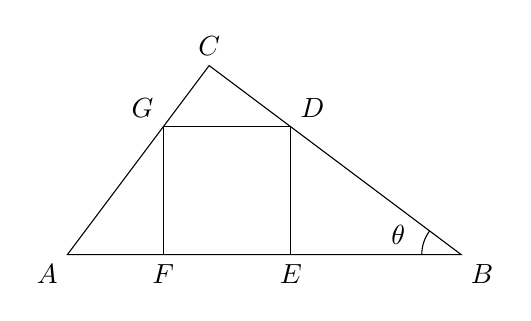
\begin{tikzpicture}[>=latex, line cap = round]
        \draw (0,0) node [below left] {$A$}-- (5,0) node [below right] {$B$}-- (9/5,12/5) node [above] {$C$}-- cycle;
        \draw (45/37,0) node [below] {$F$} -- (45/37,60/37) node [above left] {$G$}-- (105/37,60/37) node [above right] {$D$}-- (105/37,0) node [below] {$E$}; 
        \draw (5,0) ++ (180:0.5) arc (180:180-atan(3/4):0.5); 
        \draw (4.2,0) node [above] {$\theta$};
    \end{tikzpicture}
\end{center}

% 第25讲 8+2+8
\item 函数$y=2\sin(3x-\dfrac{\pi}4)$的图像的相邻两对称中心的距离是\blank{50}.
\item 设$A>0$, $\omega>0$, $0\le \varphi<2\pi$. 如图为定义在$\mathbf{R}$上的函数$f(x)=A\sin (\omega x+\varphi)$的图像的一部分, 则$f(x)$的解析式为\blank{50}.
\begin{center}
    \begin{tikzpicture}[>=latex, line cap = round, scale = 0.8]
        \draw [->] (-1,0) -- (7,0) node [below] {$x$};
        \draw [->] (0,-3) -- (0,3) node [left] {$y$};
        \draw (0,0) node [below right] {$O$};
        \draw [domain = -pi/6:25*pi/12, samples = 1000] plot (\x, {2*sin(2*\x/3/pi*180+20)});
        \draw [dashed] (7*pi/12,2) -- (0,2) node [left] {$2$};
        \draw [dashed] (25*pi/12,0) node [above] {$\dfrac{25\pi}{12}$} --++ (0,-2) -- (0,-2) node [left] {$-2$};
        \draw (-pi/6,0) node [below] {$-\dfrac{\pi}{6}$};
    \end{tikzpicture}
\end{center}
\item 要得到$y=\sin(\dfrac x2+\dfrac{\pi}4)$的图像, 可以将$y=\sin\dfrac x2$的图像\bracket{20}.
\fourch{向左平移$\dfrac{\pi}2$个单位}{向右平移$\dfrac{\pi}2$个单位}{向左平移$\dfrac{\pi}4$个单位}{向右平移$\dfrac{\pi}4$个单位}
\item 把函数$y=\sin x$的图像上所有点向左平移$\dfrac{\pi}3$个单位长度, 再把所得图像上所有点的横坐标变为原来的$\dfrac 12$(纵坐标不变), 得到的图像是函数\blank{50}的图像.
\item 若直线$x=a$与$f(x)=2\sin x$和$g(x)=3\cos x$的图像分别交于$M,N$两点, 则$|MN|$的最大值是\blank{50}.
\item 设常数$\theta\in \mathbf{R}$. 函数$f(x)=\cos(x+\theta)$是偶函数, 当且仅当$\theta=$\blank{50}.
\item 若函数$y=\tan \omega x$在$(-\dfrac{\pi}2,\dfrac{\pi}2)$上是减函数, 则实数$\omega$的取值范围是\blank{50}.
\item *设常数$t\in \mathbf{R}^+$. 若函数$y=-\sin (\dfrac{\pi }3x)$在区间$[0,t]$上恰好取得两次最大值, 则$t$的取值范围为\blank{50}.
\item 设$f(x)=A\sin(\omega x+\varphi) \ (A>0, \ \omega>0, \ -\pi<\varphi<\pi)$, $D(2,\sqrt 2)$是图像的一个最高点, 一动点从$D$出发, 沿函数图像运动至相邻的最低点. 若$P$经过点$E(6,0)$, 求$f(x)$的解析式.
\item 已知函数$f(x)=(2\sin(x+\dfrac{\pi}3)+\sin x)\cos x-\sqrt 3\sin^2 x$.\\
(1) 求函数$f(x)$的值域与周期;\\
(2) 若$x\in [0,\dfrac{\pi}2]$, 求$f(x)$的单调递减区间;\\
(3) *设常数$a>0$, 若函数$y=f(x)$的图像关于直线$x=a$对称, 求$a$的最小值;\\
(4) 设常数$m\in \mathbf{R}$, 若存在$x_0\in [0,\dfrac{5\pi}{12}]$, 使得$mf(x_0)-2=0$成立, 求$m$的取值范围.
\item 设$A\ne 0$, $\omega>0$, $-\dfrac{\pi}2<\varphi<\dfrac{\pi}2$, 函数$f(x)=A\sin(\omega x+\varphi)$的部分图像如右图所示, 则$f(x)$的解析式为\blank{50}.
\begin{center}
    \begin{tikzpicture}[>=latex, line cap = round, scale = 0.4]
        \draw [->] (-4,0) -- (11,0) node [below] {$x$};
        \draw [->] (0,-5) -- (0,5) node [left] {$y$};
        \draw (0,0) node [below right] {$O$};
        \draw [domain = -2:11, samples = 1000] plot (\x, {-4*sin(180*\x/8+45)});
        \draw [dashed] (2,-4) -- (0,-4) node [left] {$-4$} (10,4) -- (0,4) node [left] {$4$};
        \draw (-2,0) node [above] {$-2$};
        \draw (6,0) node [below] {$6$};
    \end{tikzpicture}
\end{center}
\item 函数$f(x)=\tan 2x$的图像的对称中心是\blank{50}.
\item 函数$y=\sin(2x+\dfrac{\pi}4)$图像的对称轴可以是 \bracket{20}.
\fourch{$x=-\dfrac{3\pi}4$}{$x=-\dfrac{3\pi}8$}{$x=\dfrac{3\pi}8$}{$x=\dfrac{3\pi}4$}
\item 与函数$y=\tan(2x+\dfrac{\pi}4)$没有公共点的直线可以是\bracket{20}.
\fourch{$x=-\dfrac{\pi}2$}{$x=-\dfrac{\pi}4$}{$x=\dfrac{\pi}8$}{$x=\dfrac{\pi}4$}
\item *设$\omega>0$, $0<\varphi <\pi$, 若函数$f(x)=\cos(\omega x+\varphi)$为奇函数, 且图像与直线$y=\dfrac 12$的所有交点中, 距离最近的两个交点的距离为$\pi$, 则$\omega =$\blank{50}, $\varphi=$\blank{50}.
\item *设常数$a\in \mathbf{R}$. 若函数$y=\sin 2x+a\cos 2x$的图像关于直线$x=-\dfrac{\pi}6$对称, 则$a=$\blank{50}.
\item *设常数$a\in \mathbf{R}$. 若关于$x$的方程$3\sin x+4\cos x=a$在区间$(0,2\pi)$内恰有两个相异实根$\alpha,\beta$, 求$a$的取值范围及$\alpha+\beta$的值.
\item 求函数$y=\sin^4 x+2\sqrt 3\sin x\cos x-\cos^4 x$的最小正周期和值域, 写出该函数在$[0,\pi]$上的递增区间.

% 第26讲 8+2+8
\item 求值: $\arcsin\dfrac 12=$\blank{50}; $\arccos(-\dfrac{\sqrt 2}2)=$\blank{50}; $\arctan(-\sqrt 3)=$\blank{50}.
\item 用含反三角函数的表达式表示下列各式中的角$x$:\\
(1) $\sin x=-\dfrac 13, \ x\in [-\dfrac{\pi}2,\dfrac{\pi}2]$, $x=$\blank{50};\\
(2) $\sin x=\dfrac 14, \ x\in [0,\pi]$, $x=$\blank{50};\\
(3) $\cos x=-\dfrac 14, \ x\in [0,\pi]$, $x=$\blank{50};\\ 
(4) $\cos x=\dfrac 15, \ x\in [-\pi,0]$, $x=$\blank{50};\\
(5) 三角形$ABC$中, $\sin A=\dfrac 14$, $\tan B=-2$, 则$A=$\blank{50}, $B=$\blank{50}.
\item 设$|a|\le 1$, 则$\arccos a+\arccos(-a)=$\blank{50}.
\item 化简下列各式: $\sin(\arcsin\dfrac 1{a^2+1})=$\blank{50}; $\cos(\arcsin(-\sqrt{1-a^4}))=$\blank{50}; $\cot(\arctan\dfrac 1a)=$\blank{50}.
\item 函数$y=\sin x, \ x\in [-\dfrac{\pi}2,\dfrac{\pi}4]$的反函数是\blank{50}.
\item 满足不等式$\arccos(1-x)\ge \arccos x$的$x$的取值范围是\blank{50}.
\item 函数$y=(\arctan x)^2+\arctan x-1$的最小值是\blank{50}.
\item 方程$2\sin x=1, \ x\in [-2\pi,2\pi]$的解集是\blank{50}.
\item 研究函数$y=\arccos(x-x^2)$的定义域, 值域, 单调性, 并给出单调性的严格证明.
\item 解下列三角方程:\\
(1) $\sin 2x=\sin 5x$;\\
(2) $\sin 2x-\sqrt 3\cos 2x=1, \ x\in [-\pi,\pi]$;\\
(3) $\dfrac{\sin 2x}{\cos x+\sin x}=4$;\\
(4) $\tan 2x=\tan 6x$;\\
(5) $\sin^2 x-4\sin x\cos x+2\cos^2 x=-\dfrac 12$.
\item 下列等式成立的是\blank{50}(填序号).\\
\textcircled{1} $\arccos 0=1$; \textcircled{2} $\cos(\arccos \dfrac{\pi}2)=\dfrac{\pi}2$; \textcircled{3} $\sin(\arcsin\dfrac{\pi}4)=\dfrac{\pi}4$; 
\textcircled{4} $\arctan\dfrac{\pi}3=\sqrt 3$; \textcircled{5} $\tan(\arctan\dfrac{\pi}2)=\dfrac{\pi}2$.
\item 若$\cos\alpha=-\dfrac 34$, $\alpha\in (\pi,\dfrac{3\pi}2)$, 则$\alpha=$\blank{50}.
\item 设$x=\sin\alpha$, $\alpha\in (-\dfrac{\pi}6,\dfrac{5\pi}6]$, 则$\arccos x$的取值范围为\blank{50}.
\item 方程$2\sin^2 x+5\sin x+2=0$在$(-2\pi,0)$上的解集为\blank{50}.
\item 方程$2\sin^2 x-3\sin x\cos x-2\cos^2 x=0$的解集为\blank{50}.
\item 若$\tan x=a, \ x\in (\dfrac{\pi}2,\pi)$, 则$x=$\blank{50}.
\item 若$-\pi<x<-\dfrac{\pi}2$, 则$\arcsin(\sin x)=$\blank{50}.
\item 设常数$m\in \mathbf{R}$, 关于$x$的方程$2-\sin 2x=m(2+\sin 2x), \ x\in [0,\pi)$的解集为$A$.\\
(1) 若$A\ne \varnothing$, 求$m$的取值范围;\\
(2) 若$A\subseteq (0,\pi)$, 且$A$中至少有两个元素, 求$m$的取值范围.

% 第27讲 8+3+7
\item 写出下列数列的一个通项公式:\\
(1) $-3,1,5,9,13,\cdots$: $a_n$=\blank{50}; (2)$\dfrac 27,\dfrac 4{11},\dfrac 12,\dfrac 45,2$: $a_n$=\blank{50}.
\item 已知数列$\{a_n\}$满足: $a_n=n+\dfrac 6n$, 则数列$\{a_n\}$中最小项为第\blank{50}项.
\item (1) 数列$\{a_n\}$满足:  $a_1+a_2+a_3+\cdots +a_n=8$, 则$a_n=$\blank{50};\\
(2) 数列$\{a_n\}$满足:  $a_1\cdot a_2\cdot a_3\cdots a_n=8$, 则$a_n=$\blank{50}.
\item 已知$a_1=1$, $a_2=3$, $a_{n+2}=a_{n+1}-a_n$, 则$a_{2030}=$\blank{50}.
\item 数列$\{a_n\}$满足$a_{n+1}=\begin{cases}2a_n,&  0\le a_n<\dfrac 12,\\ 2a_n-1, &\dfrac 12\le a_n<1. \end{cases}$ 若$a_1=\dfrac 67$, 则$a_2=$\blank{50}; $a_3=$\blank{50}; $a_{2021}=$\blank{50}.
\item 已知数列$\{a_n\}$和$\{b_n\}$, 其中$a_n=n^2$, $n\in \mathbf{N}^*$, $\{b_n\}$的项是互不相等的正整数, 若对于任意$n\in \mathbf{N}^*$, $\{b_n\}$的第$a_n$项等于$\{a_n\}$的第$b_n$项, 则$\dfrac{\lg (b_1b_4b_9b_{16})}{\lg (b_1b_2b_3b_4)}=$\blank{50}.
\item 已知数列$\{a_n\}$的通项$a_n=n+\mathrm{e}^n$.\\
(1) 把该数列的前$10$项去掉, 得到新数列$\{b_n\}$, 则通项$b_n=$\blank{50};\\
(2) 将该数列的奇数项按原来的先后顺序排列, 得到新数列$\{c_n\}$, 则通项${c_n}=$\blank{50}.
\item 已知数列$\{a_n\}$的前$n$项和是$S_n=2\cdot 3^n+3$, 求数列$\{a_n\}$的通项$a_n$.
\item 已知数列$\{a_n\}$的通项$a_n=(n+1)(\dfrac{10}{11})^n$, 试问该数列有没有最大项? 若有, 求出最大项; 若没有, 说明理由.
\item 已知$\{a_n\}$是递增数列, 且$a_n=n^2+\lambda n$, 求实数$\lambda$的取值范围.
\item 已知数列$\{a_n\}$的通项$a_n=2^n$. 对任意的$k\in \mathbf{N}^*$, 在$a_{2k}$与$a_{2k+1}$中间插入一项$k$, 构成新数列$\{b_n\}:2,4,1,8,16,2,32,64,3,128,\cdots$. 求数列$\{b_n\}$的通项公式.
\item 已知数列$\{a_n\}$满足$a_{n+2}=a_n$, ${a_1}=1$, ${a_2}=2$, 则通项$a_n=$\blank{50}.
\item 已知数列$\{a_n\}$满足$a_{n+1}=a_n^2-k$, $a_1=1$, $a_3=-1$, 则常数$k=$\blank{50}.
\item 已知数列$\{a_n\}$满足: $a_n=\dfrac 1{n-5.5}$, 则此数列中最大项的值为\blank{50}, 最小项的值为\blank{50}.
\item 已知数列$\{a_n\}$满足: $a_n=2^n$, 删去数列中第$1,4,\cdots,3n-2,\cdots$项, 得到新数列的通项$b_n=$\blank{50}.
\item 无穷数列$\{a_n\}$由$k$个不同的数组成, $S_n$为$\{a_n\}$的前$n$项和, 若对任意$n\in \mathbf{N}*$, $S_n\in \{2,3\}$, , 则$k$的最大值为\blank{50}.
\item 设$\lambda$是实常数, 数列$\{a_n\}$的通项$a_n=n+\dfrac{\lambda}n$.\\
(1) 若数列$\{a_n\}$递增, 求$\lambda$的取值范围;\\
(2) 若数列$\{a_n\}$中, 唯一最小项为$a_4$, 求$\lambda$的取值范围.
\item 已知正项数列$\{a_n\}$满足$a_n-\dfrac 1a_n=-2n$, 求证: 数列$\{a_n\}$是递减数列.

%第28讲 8+3+7
\item 等差数列$\{a_n\}$中, 已知$a_1=3$, $d=2$, 则通项$a_n=$\blank{50}, 前$n$项和$S_n=$\blank{50}.
\item 等差数列$\{a_n\}$中, 已知$a_1=3$, $a_2+a_5=-4$, $a_n=-11$, 则$n=$\blank{50}.
\item 记等差数列$\{a_n\}$的前$n$项和为$S_n$, 若$a_3=0$, $a_7+a_8=0$, 则$S_7=$\blank{50}.
\item 等差数列$\{a_n\}$中, 已知$a_1=1$, $a_1+a_2+a_5=13$, 则前$n$项和$S_n=$\blank{50}.
\item 已知等差数列$\{a_n\}$的前$n$项之和为$S_n$, 若$S_{15}$为一确定常数, 则下列各式也为确定常数的是\bracket{20}.
\fourch{$a_2+a_{13}$}{$a_2\cdot a_{13}$}{$a_1+a_8+a_{15}$}{$a_1\cdot a_8\cdot a_{15}$}
\item 在$a$和$b$($a<b$)之间插入$n$个数, 使这$n+2$个数组成递增的等差数列, 则该数列的公差为\blank{50}.
\item 已知数列$\{a_n\}$的通项为$a_n=\sqrt{99}-n$, 前$n$项和为$S_n$, 则\\
(1) $\{a_n\}$中最后一个为正数的项是第\blank{50}项;\\
(2) 数列$\{S_n\}$中, 第\blank{50}项最大.
\item 设数列$\{a_n\}$中, $a,b$为常数. 在下列三个条件中: \textcircled{1} $a_{n+1}-a_n=a$; \textcircled{2} $2a_{n+1}=a_n+a_{n+2}$; \textcircled{3} $a_n=an+b$, 可推出$\{a_n\}$是等差数列的条件为\blank{50}(填入序号).
\item 已知数列$\{a_n\}$为等差数列, 公差为$d$. 求证: 数列$\{2a_{2n}\}$也是等差数列.
\item 已知数列$\{a_n\}$的前$n$项和是$S_n=an^2+bn+c$, 其中$a,b,c$为常数, 若数列$\{a_n\}$为等差数列, 求实数$a,b,c$应满足的条件.
\item 设等差数列$\{a_n\}$的前$n$项和为$S_n$, 已知$a_2=6$, $S_6>0$, $S_7<0$.\\
(1) 求公差$d$的取值范围;\\
(2) 数列$\{S_n\}$是否有最大项? 若有, 求出该项为第几项; 若无, 说明理由.
\item 等差数列$\{a_n\}$中, $a_1+a_4+a_7=9$, $a_2+a_5+a_8=3$, 则$a_3+a_6+a_9=$\blank{50}.
\item 设$S_n$为等差数列$\{a_n\}$的前n项和, 若$S_5=10$, $S_{10}=-5$, 则$S_{15}=$\blank{50}.
\item 设$a$是实数, 若等差数列$\{a_n\}$的前$n$项和$S_n=n+a$, 则$a=$\blank{50}.
\item 已知等差数列$\{a_n\}$, $\{b_n\}$的前$n$项和分别为$S_n,T_n$, 若$\dfrac{S_n}{T_n}=\dfrac{n-1}{n+1}$, 则$\dfrac{a_8}{b_8}=$\blank{50}.
\item 等差数列$\{a_n\}$中, $S_n$为前$n$项和, 且$S_6<S_7$,$S_7>S_8$, 给出下列命题:\\
(1) 数列$\{a_n\}$中前$7$项是递增的, 从第$8$项开始递减;
(2) $S_9$一定小于$S_6$;
(3) $a_1$是$\{a_n\}$各项中的最大的;
(4) $S_7$不一定是$\{S_n\}$中最大项. 其中正确的序号是\blank{50}.
\item 设等比数列$\{b_n\}$各项为正, 数列$\{a_n\}$满足: $a_n=\dfrac{\lg b_1+\lg b_2+\cdots+\lg b_n}n$, 证明: 数列 $\{a_n\}$为等差数列.
\item 设数列$\{a_n\}$的通项公式为$a_n=pn+q$($n\in \mathbf{N}^*, \ p>0$). 数列$\{b_n\}$定义如下: 对于正整数$m$, $b_m$是使得不等式$a_n>m$成立的所有$n$中的最小值.\\
(1) 若$p=\dfrac{1}{2}$, $q=-\dfrac{1}{3}$求$b_3$;\\
(2) 若$p=2$, $q=-1$, 求数列$\{b_n\}$的前$2m$项和公式.

% 第29讲 8+3+7
\item 实数组成的等比数列$\{a_n\}$中, 已知$a_1=2$, $a_4=54$, 则通项$a_n=$\blank{50}.
\item 等比数列$\{a_n\}$中, $a_1=4$, $a_2=2$, 则$a_1a_2+a_2a_3+\cdots +a_na_{n+1}=$\blank{50}.
\item 已知数列$\{a_n\}$是等比数列, 且$a_n>0$, 若$b_n=\log_2a_n$, 则\bracket{20}
\twoch{$\{b_n\}$一定是递增的等差数列}{$\{b_n\}$不可能是等比数列}{$\{b_n+1\}$一定是等差数列}{$\{3^b_n\}$不是等比数列}\item 等比数列$\{a_n\}$满足$a_1=1$, $a_3=81$, 则$a_2=$\blank{50}.
\item 若实数$a$、$b$、$c$、$d$、$e$依次构成等比数列, 且$a=-1$, $e=-81$, 则$c$=\blank{50}.
\item 若等比数列$\{a_n\}$的前$n$项和为$S_n=3^n+a$, 则实数$a=$\blank{50}.
\item 设等差数列$\{a_n\}$的前$n$项和为$S_n$, 则$S_4,S_8-S_4,S_{12}-S_8,S_{16}-S_{12}$成等差数列. 类比以上结论有: 设等比数列$\{b_n\}$的前$n$项积为$T_n$, 则$T_4$,\blank{50}, \blank{50}, $\dfrac{T_{16}}{T_{12}}$成等比数列.
\item 几位大学生响应国家的创业号召, 开发了一款应用软件. 为激发大家学习数学的兴趣, 他们推出了``解数学题获取软件激活码''的活动. 这款软件的激活码为下面数学问题的答案: 已知数列$1, 1, 2, 1, 2, 4, 1, 2, 4, 8, 1, 2, 4, 8, 16, \cdots$, 其中第一项是$2^0$, 接下来的两项是$2^0,2^1$, 再接下来的三项是$2^0,2^1,2^2$, 依此类推.求满足如下条件的最小整数$N$($N>100$), 且该数列的前$N$项和为2的整数幂.那么该款软件的激活码是\bracket{20}.
\fourch{$440$}{$330$}{$220$}{$110$}
\item 已知由实数组成的数列$\{a_n\}$, 前$n$项和记为$S_n$, 若数列$\{a_n\}$为等比数列, $S_{100}=100S_{50}$, 求$\dfrac{a_{100}}{a_{50}}$的值.
\item 已知数列$\{c_n\}$, 其中$c_n=2^n+3^n$, 是否存在实数$p$使得数列$\{c_{n+1}-p{c_n}\}$为等比数列, 若存在, 求出$p$; 若不存在, 说明理由.
\item 已知等比数列$\{a_n\}$中每一项均为实数, 设数列$\{a_n\}$的前$n$项和为$S_n$.\\
(1) 证明: $(S_{2n}-S_n)^2=S_n(S_{3n}-S_{2n})$;\\
(2) 试给出一个例子使得$S_n,S_{2n}-S_n,S_{3n}-S_{2n}$依次不构成等比数列;\\
(3) 若$S_{10}=2$, $S_{30}=14$, 求$S_{20}$.
\item 等比数列$\{a_n\}$满足$a_1=2$, $a_2=1$, 则通项$a_n=$\blank{50}.
\item 若等比数列$\{a_n\}$的公比为$3$, 则等比数列$\{a_n\cdot a_{n+3}\}$的公比为\blank{50}.
\item 若实数$a$使得$a,a^2,a$依次构成等比数列, 则$a=$\blank{50}.
\item 若数列$\{a_n\}$为等差数列, 则$a_9=4a_3-3a_1$. 类比以上结论有: 若数列$\{b_n\}$为等比数列, 则$b_9=$\blank{50}.
\item 设$\{a_n\}$是各项为正数的无穷数列, $A_i$是边长为$a_i$、$a_{i+1}$的矩形的面积($i=1,2,\cdots$), 则$\{a_n\}$为等比数列的充要条件是\bracket{20}.
\onech{$\{a_n\}$是等比数列}{$a_1,a_3,\cdots,a_{2n-1},\cdots$或$a_2,a_4,\cdots,a_{2n},\cdots$是等比数列}{$a_1,a_3,\cdots,a_{2n-1},\cdots$和$a_2,a_4,\cdots,a_{2n},\cdots$均是等比数列}{$a_1,a_3,\cdots,a_{2n-1},\cdots$和$a_2,a_4,\cdots,a_{2n},\cdots$均是等比数列, 且公比相同}
\item 设$p\in \mathbf{R}$, 已知数列$\{a_n\}$满足$a_1=1$, $a_{n+1}=a_n^2-p$, 是否存在$p$使得$\{a_n\}$是等比数列? 若存在, 求出$p$的值; 若不存在, 说明理由.
\item 设数列$\{a_n\}$的前$n$项和为$S_n$, 已知$a_1=1$, $S_{n+1}=4a_n+2$.\\
(1) 设$b_n=a_{n+1}-2a_n$, 证明数列$\{b_n\}$是等比数列;\\
(2) 求数列$\{a_n\}$的通项公式.




% 第30讲 8+3+7
\item 求和: $\sin^21^\circ +\sin^22^\circ+\sin^23^\circ+\cdots+\sin^288^\circ+\sin^289^\circ=$\blank{50}.
\item 设$f(x)=\dfrac 1{3^x+\sqrt 3}$, 利用课本中推导等差数列前$n$项和的公式的方法, 可求得$f(-5)+f(-4)+\cdots+f(0)+\cdots+f(5)+f(6)$的值为\blank{50}.
\item 已知数列$\{a_n\}$的通项$a_n=1+2+2^2+\cdots+2^n$, 则其前$n$项和$S_n=$\blank{50}.
\item 已知数列$\{a_n\}$的通项$a_n=\dfrac 1{(2n-1)(2n+1)}$, 则其前$n$项和$S_n=$\blank{50}.
\item 已知数列$\{a_n\}$的通项$a_n=\dfrac 3{n(n+3)}$, 则其前$n$项和$S_n$=\blank{50}.
\item 等比数列$\{a_n\}$中前$n$项和为$S_n$, $n\in \mathbf{N}^*$, 若$S_n=48$, $S_{2n}=60,$则$S_{4n}=$\blank{50}.
\item 在等差数列$\{a_n\}$中, 满足$3a_4=7a_7$, 且$a_1>0$, $S_n$是数列$\{a_n\}$前$n$项的和, 若$S_n$取得最大值, 则$n=$\blank{50}.
\item 已知数列$\{a_n\}$的通项$a_n=n\cdot 2^n$, 求其前$n$项和$S_n$.
\item 已知数列$\{a_n\}$的前$n$项和为$S_n=n^2-20n$, 求数列$\{|a_n|\}$的前$n$项和$T_n$.
\item 求数列$\{\dfrac{(n+1)^2+1}{(n+1)^2-1}\}$的前$n$项和$S_n$.
\item (1) 设$n$为正整数, 求和: $1-3+5-7+9+\cdots +(-1)^{n-1}\cdot (2n-1)$;\\
(2) 已知数列$\{a_n\}$的通项$a_n=\begin{cases}3n+1, & n\text{为奇数}, \\ 2^{\frac n2}, & n\text{为偶数},  \end{cases}$ 求其前$n$项和$S_n$.
\item 数列$\{a_n\}$的通项$a_n=2^n\cdot 3^n$, 则其前$n$项和$S_n=$\blank{50}.
\item 已知数列$\{a_n\}$的通项$a_n=\dfrac 2{\sqrt{n+2}+\sqrt n}$, 则其前$n$项和$S_n=$\blank{50}.
\item 等差数列$\{a_n\}$的前$n$项和为$S_n$, $a_3=3$, $S_4=10$, 则数列$\{S_n\}$的前$n$项和为\blank{50}.
\item 求数列$\{\dfrac n{2^n}\}$的前$n$项和$S_n$.
\item 已知数列$\{a_n\}$满足$a_n=\begin{cases}n, & n
\text{是奇数}, \\ 2^n, & n\text{是偶数}. \end{cases}$ 试求数列$\{a_n\}$的前$n$项和$S_n$.
\item 如果有穷数列$a_1,a_2,a_3,\cdots,a_m$($m$为正整数)满足条件$a_1=a_m$, $a_2=a_{m-1}$, $\cdots$, $a_m=a_1$, 即$a_i=a_{m-i+1}$($i=1,2,\cdots,m$), 我们称其为``对称数列''.  例如数列$1,2,5,2,1$与数列$8,4,2,2,4,8$都是``对称数列''.\\
(1) 设$\{c_n\}$是$49$项的``对称数列'', 其中$c_{25},c_{26},\cdots,c_{49}$是首项为$1$, 公比为$2$的等比数列, 求$\{c_n\}$各项的和$S$;\\
(2) 设$\{d_n\}$是$100$项的``对称数列'', 其中$d_{51},d_{52}\cdots,d_{100}$是首项为$2$, 公差为$3$的等差数列. 求$\{d_n\}$前$n$项的和$S_n$($n=1,2,\cdots,100$).
\item 设数列$\{a_n\}$满足$a_1=0$且$\dfrac 1{1-a_{n+1}}-\dfrac 1{1-a_n}=1$.\\
(1) 求$\{a_n\}$的通项公式;\\
(2) 设$b_n=\dfrac{1-\sqrt{a_{n+1}}}{\sqrt n}$, 记$S_n={b_1}+{b_2}+\cdots +b_n$, 求$\{S_n\}$的通项公式.



% 第31讲 7+3+6

\item 数学归纳法证明$1+a+a^2+\cdots+a^{n+1}=\dfrac{1-a^{n+2}}{1-a}\ (a\ne 1)$, 在验证$n=1$时, 左边计算所得项为\blank{50}.
\item 用数学归纳法证明``对于任意正偶数$n$, $a^n-b^n$能被$a+b$整除''时, 其第二步论证应该是\bracket{20}.
\onech{假设$n=k$, $k\in \mathbf{N}^*$时命题成立, 证明$n=k+1$时, 命题也成立}{假设$n=2k$, $k\in \mathbf{N}^*$时命题成立, 证明$n=2k+1$时, 命题也成立}{假设$n=k$, $k\in \mathbf{N}^*$时命题成立, 证明$n=k+2$时, 命题也成立}{假设$n=2k$, $k\in \mathbf{N}^*$时命题成立, 证明$n=2k+2$时, 命题也成立}\item 用数学归纳法证明: $1^2-2^2+3^2-4^2+\cdots+(2n-1)^2-(2n)^2=-n(2n+1)$, $n$从$k$到$k+1$时, 等式左边增加的项为\blank{50}.
\item 根据$1=1$, $1-4=-(1+2)$, $1-4+9=1+2+3$, $1-4+9-16=-(1+2+3+4)$, $\cdots$, 请写一个能体现其一般规律的数学表达式:\blank{50}.
\item 设$f(x)$是定义在正整数集上的函数, 且$f(x)$满足: ``当$f(k)\ge k^2$成立时, 总可推出$f(k+1)\ge (k+1)^2$成立''. 那么, 下列说法中正确的是\bracket{20}.
\onech{若$f(3)\ge 9$成立, 则当$k\ge 1$时, 均有$f(k)\ge k^2$成立}{若$f(5)\ge 25$成立, 则当$k\le 5$时, 均有$f(k)\ge k^2$成立}{若$f(7)<49$成立, 则当$k\ge 8$时, 均有$f(k)<k^2$成立}{若$f(4)=25$成立, 则当$k\ge 4$时, 均有$f(k)\ge k^2$成立 }
\item 已知数列$\{a_n\}$满足$a_1=2$, $a_{n+1}=\dfrac{1-a_n}{1+a_n}$, 则$\{a_n\}$的通项$a_n=$\blank{50}.
\item 已知数列$\{a_n\}$满足$a_1=1$, $a_{n+1}=n+\dfrac 2{a_n-n+2}$, 猜测$\{a_n\}$的通项, 并用数学归纳法证明.
\item 是否存在实数$a$, 使得等式$\dfrac 1{1^2}+\dfrac 1{2^2}+\cdots +\dfrac 1{n^2}=\dfrac{an}{3n-1}$对一切正整数$n$成立? 请说明理由.
\item 用数学归纳法证明: 对一切正整数$n$, $5^n+12n-1$是$16$的倍数.
\item 正数数列$\{a_n\}$前$n$项和为$S_n$, 若$S_n=\dfrac 12(a_n+\dfrac 1{a_n})$.\\
(1) 求$a_1,a_2,a_3$的值;\\
(2) 猜测通项$a_n$, 并用数学归纳法加以证明.
\item 数学归纳法证明: $1-\dfrac 12+\dfrac 13-\dfrac 14+\cdots +\dfrac 1{2n-1}-\dfrac 1{2n}=\dfrac 1{n+1}+\dfrac 1{n+2}+\cdots +\dfrac 1{2n}$时, 当$n$从$k$到$k+1$时等式右边增加与减少的项分别为\blank{50}, \blank{50}.
\item 若$S_n=1+\dfrac 12+\dfrac 13+\cdots +\dfrac 1n$, 用数学归纳法证明: $S_{2^n}>1+\dfrac n2\ (n\ge 2)$, $n$从$k$到$k+1$时, 不等式左边增加的项为\blank{50}.
\item 根据 $1=1$, $2+3+4=9$, $3+4+5+6+7=25$, $\cdots$, 请写一个能体现其一般规律的数学表达式:\blank{50}.
\item (1) 已知数列$\{a_n\}$满足$a_1=3$, $a_{n+1}=a_n^2-2\ (n\in \mathbf{N}^*)$. 求证: 当$n\in \mathbf{N}^*$时, $a_n\ge 3$;\\
(2) *已知数列$\{a_n\}$满足$a_n\ge 0$, $a_1=0$, $a_{n+1}^2+a_{n+1}-1=a_n^2 \ (n\in \mathbf{N}^*)$. 求证: 当$n\in \mathbf{N}^*$时, $a_n<a_{n+1}$.
\item 在数列$\{a_n\}$, $\{b_n\}$中, $a_1=2$, $b_1=4$, 且$a_n,b_n,a_{n+1}$成等差数列, $b_n,a_{n+1},b_{n+1}$成等比数列($n\in \mathbf{N}^*)$. 写出$a_2,a_3,a_4$及$b_2,b_3,b_4$的值, 由此猜测$\{a_n\}$, $\{b_n\}$的通项公式, 并证明你的结论.
\item (1) 用数学归纳法证明: 对一切正整数$n$, $2^{n+2}\cdot 3^n+5n+21$能被$25$整除;\\
(2) *是否存在大于$1$的正整数$m$, 使得对于任意正整数$n$, $f(n)=(2n+7)\cdot 3^n+9$都能被$m$整除? 若存在, 求出$m$的最大值, 并证明你的结论; 若不存在, 说明理由.


% 第32讲 8+3+8

\item 数列$\{a_n\}$中, $a_n=\begin{cases}\dfrac 1{n^2}, & 1\le n\le 10^{10},  \\ \dfrac{2020n^2}{2020n^2-2022n}, & n\ge 10^{10},\end{cases}$ 则数列$\{a_n\}$的极限值\bracket{20}.
\fourch{等于$0$}{等于$1$}{等于$0$或$1$}{不存在}
\item (1) $\displaystyle\lim_{n\to \infty}(\dfrac{n^2+1}n-\dfrac{n^2}{n+1})=$\blank{50};\\
(2) 设$m\in \mathbf{N}^*$, 则$\displaystyle\lim_{n\to \infty}(\dfrac mn-\dfrac 1{n+1}-\dfrac 1{n+2}-\dfrac 1{n+3}-\cdots -\dfrac 1{n+m})=$\blank{50}.
\item 设等比数列$\{a_n\}$的通项公式为$a_n={q^{n+1}}$($n\in \mathbf{N}^*$), 前$n$项和为$S_n$.若$\displaystyle\lim_{n\to \infty}\dfrac {S_n}{a_{n+1}}=\dfrac 12$, 则$q$=\blank{50}
 \item 设$a$是实常数, 则:\\
(1) $\displaystyle\lim_{n\to \infty}\dfrac{2an^2+n+1}{an^2-n+1}=$\blank{50};\\
(2) $\displaystyle\lim_{n\to \infty}\dfrac{1-2a^n}{1+a^n}=$\blank{50}($a\ne -1$).
\item 无穷等比数列$\{a_n\}$的前$n$项和为$S_n$, 则数列$\{a_n\}$有极限是数列$\{S_n\}$有极限的\bracket{20}条件.
\fourch{充分不必要}{必要不充分}{充要}{既不充分又不必要}
\item 化简: $0.\dot1\dot6=$\blank{50}; $0.1\dot6$=\blank{50};
 $0.1\dot6+0.01\dot6+0.001\dot6+\cdots$=\blank{50}(用最简分数表示)
. 
\item 如图, 正方形$ABCD$边长为1, 联结该正方形各边的中点得到一个新的正方形$A_1B_1C_1D_1$, 再在正方形$A_1B_1C_1D_1$中用同样的方法得到又一个新的正方形$A_2B_2C_2D_2$, 这样无限地继续下去, 则所有这些得到的新正方形面积之和为\blank{50}.
\begin{center}
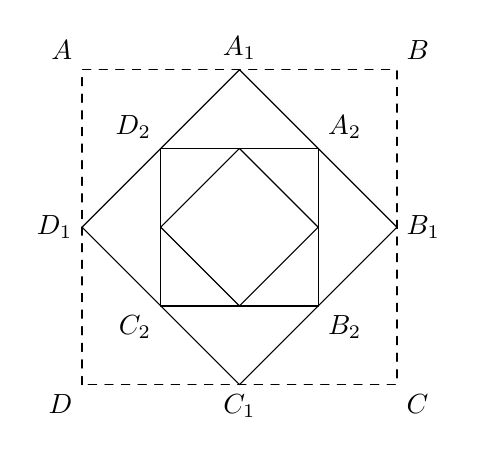
\begin{tikzpicture}[>=latex, line cap = round, line join = round]
    \draw [dashed] (0,0) rectangle (4,4);
    \draw (0,2) -- (2,4) -- (4,2) -- (2,0) -- cycle;
    \draw (1,3) -- (3,3) -- (3,1) -- (1,1) -- cycle;
    \draw (2,3) -- (3,2) -- (2,1) -- (1,2) -- cycle;
    \draw (0,4) node [above left] {$A$} (4,4) node [above right] {$B$} (4,0) node [below right] {$C$} (0,0) node [below left] {$D$};
    \draw (2,4) node [above] {$A_1$} (4,2) node [right] {$B_1$} (2,0) node [below] {$C_1$} (0,2) node [left] {$D_1$};
    \draw (3,3) node [above right] {$A_2$} (3,1) node [below right] {$B_2$} (1,1) node [below left] {$C_2$} (1,3) node [above left] {$D_2$};
\end{tikzpicture}
\end{center}
\item 已知公比为$q(0<q<1)$的无穷等比数列$\{a_n\}$各项的和为$9$, 无穷等比数列$\{a_n^2\}$各项的和为$\dfrac{81}5$.则数列$\{a_n\}$的首项$a_1=$\blank{50}, 公比$q$=\blank{50}.
\item 已知$a_n=\begin{cases} \dfrac 1{2^n}, & n\text{为奇数}, \\ \dfrac 1{3^n}, & n\text{为偶数}, \end{cases}$ 求$\displaystyle\lim_{n\to \infty}(a_1+a_2+\cdots +a_{2n})$.
\item 已知$a,b,c$是实数, $\displaystyle\lim_{n\to \infty}\dfrac{an+1}{bn+3}=\dfrac 13$, $\displaystyle\lim_{n\to \infty}\dfrac{bn^2-4}{cn^2+2}=-2$. 求$\displaystyle\lim_{n\to \infty}\dfrac{an^3+2n+5}{cn^3+4n+3}$.
\item 设$\{a_n\}$是首项为$a$, 公比为$q(q>0)$的等比数列, 前$n$项和为$S_n$, 若$G_n=a_1^2+a_2^2+\cdots+a_n^2$, 求$\displaystyle\lim_{n\to \infty}\dfrac{S_n}{G_n}$.
\item 设无穷等比数列$\{a_n\}$满足$\displaystyle\lim_{n\to \infty}(a_1+a_3+a_5+\cdots +a_{2n-1})=\dfrac 83$, 则首项$a_1$的取值范围为\blank{50}.
\item (1) $\displaystyle\lim_{n\to \infty}\dfrac{(-2)^n+1}{(-2)^{n+1}+1}$=\blank{50};\\
(2) $\displaystyle\lim_{n\to \infty}\dfrac{6-2+4-8+\cdots+(-2)^{n+1}}{4+3+9+27+\cdots+3^n}$=\blank{50}.
\item (1)若$\displaystyle\lim_{n\to \infty}(\dfrac{n^3-1}{2n^2+n}-an-b)=0$, 则$a$=\blank{50}, $b$=\blank{50};\\
(2) 若$\displaystyle\lim_{n\to \infty}\dfrac{5^n}{5^{n+1}+(a+1)^n}=\dfrac 15$, 则实数$a$的取值范围是\blank{50}.
\item 设$\{a_n\}$为无穷等比数列, 若$\{a_n\}$的任意一项都是它后面所有项和的$4$倍, 则公比为\blank{50}.
\item 已知无穷等比数列$\{a_n\}$的公比为$q$, 前$n$项和为$S_n$, 且$\displaystyle\lim_{n\to \infty}S_n=S$, 下列条件中, 使得$2S_n<S$($n\in \mathbf{N}*$)恒成立的是\bracket{20}.
\twoch{$a_1>0,\ 0.6<q<0.7$}{$a_1<0,\ -0.7<q<-0.6$}{$a_1>0, \ 0.7<q<0.8$}{$a_1<0,\ -0.8<q<-0.7$}
\item 设等差数列$\{a_n\}$的公差为$d$, 若$a_n$恒不为零, 求$\displaystyle\lim_{n\to \infty}\dfrac{S_n}{na_n}$.
\item 已知等差数列$\{a_n\}$的首项为$1$, 公差为$d$, 前$n$项的和为$A_n$; 等比数列的首项为$1$, 公比为$q$, $|q|<1$, 前$n$项的和为$B_n$, 记$S_n=B_1+B_2+\cdots+B_n$, 若$\displaystyle\lim_{n\to \infty}(\dfrac{a_n}n-S_n)=1$, 求$d$、$q$.
\item 已知数列$\{a_n\}$是公差不为$0$的等差数列, $a_1=\dfrac 12$, 数列$\{b_n\}$是等比数列, 且$b_1=a_1$, $b_2=a_3$, $b_3=a_4$. 数列$\{b_n\}$的前$n$项和为$S_n$, 记点${Q_n}(b_n,S_n)$, $n\in \mathbf{N}*$.\\
(1) 求数列$\{b_n\}$的通项公式;\\
(2) 证明点$Q_1,Q_2,\cdots,Q_n,\cdots$在同一条直线$l$上, 并求出直线$l$的方程;\\
(3) 若记$\triangle OQ_nQ_{n+1}$($n\in \mathbf{N}*$)的面积为$a_n$, 且${T_n}$为数列$\{a_n\}$的前$n$项和, 求$\displaystyle\lim_{n\to \infty}a_n$、$\displaystyle\lim_{n\to \infty}T_n$.
 

%第33讲 7+3+7


\item 数列$\{a_n\}$满足: $a_1=1$, $a_{n+1}=a_n+2^n$, 则$a_n=$\blank{50}.
\item 数列$\{a_n\}$满足: $a_1=1$, $a_{n+1}=2^na_n$, 则$a_n=$\blank{50}.
\item 数列$\{a_n\}$满足: $a_1=2$, $a_{n+1}=\sqrt a_n$, 则$a_n=$\blank{50}.
\item 数列$\{a_n\}$满足: $a_1=3$, $a_{n+1}=4a_n+6$, 则$a_n=$\blank{50}.
\item 数列$\{a_n\}$及前$n$项和$S_n$满足: $S_n=2a_n+n-4$, 则$a_n$=\blank{50}.
\item 数列$\{a_n\}$及前$n$项和$S_n$满足: $a_1=3$, $S_{n-1}=a_n+n$, $n\ge 2$, 则$a_n=$\blank{50}.
\item 数列$\{a_n\}$满足: $a_1=1$, $a_{n+1}=\dfrac{2a_n}{a_n+4}$, 则$a_n=$\blank{50}.
\item 已知数列$\{a_n\}$满足$a_1=3$, $a_n\times a_{n+1}=(\dfrac 12)^n$, 求此数列的通项$a_n$.
\item 数列$\{a_n\}$满足$a_1=\dfrac 35$, $a_n=2-\dfrac 1{a_{n-1}}$, 数列$\{b_n\}$满足$b_n=\dfrac 1{a_n-1}$.\\
(1) 求证: 数列$\{b_n\}$是等差数列;\\
(2) 求数列$\{a_n\}$的通项.
\item 数列$\{a_n\}$的首项为$\dfrac 12$, 且前$n$项和$S_n$和$a_n$满足: 当$n\ge 2$时, $S_n^2=a_n(S_n-1)$, 求$a_n$、$S_n$.
\item 已知数列$\{a_n\}$满足$a_1=1$, $a_{n+1}+a_n=8$, 则通项$a_n=$\blank{50}.
\item 已知数列$\{a_n\}$满足$a_1=1$, $a_n=a_1+2a_2+3a_3+\cdots+(n-1)a_{n-1}$, $n\ge 2$, 则通项$a_n=$\blank{50}.
\item 已知数列$\{a_n\}$满足$a_n=\begin{cases} 5, & n=1, \\ a_1+a_2+...+a_{n-1}, & n\ge 2. \end{cases}$ 则通项$a_n=$\blank{50}.
\item 已知数列$\{a_n\}$满足: $a_1=3$, $a_{n+1}=-2a_n+6$, 求$a_n$.
\item 数列$\{a_n\}$中, $a_1=1$, $a_2=2$, 且$a_{n+1}=(1+q)a_n-qa_{n-1}$($n\ge 2, \ q\ne 0$).\\
(1) 设$b_n={a_{n+1}}-a_n$($n\in \mathbf{N}^*$), 证明$\{b_n\}$是等比数列;\\
(2) 求数列$\{a_n\}$的通项公式.
\item 设数列$\{a_n\}$的前$n$项和为$S_n$, 满足$6S_n=(a_n+1)(a_n+2)$.\\
(1) 若$a_n>0$, 求通项$a_n$;
(2) (不需要理由)试写出所有可能的数列$\{a_n\}$的前三项.
\item 已知数列$\{a_n\}$和$\{b_n\}$满足: $a_1=\lambda$, $a_{n+1}=\dfrac 23a_n+n-4$, $b_n=(-1)^n(a_n-3n+21)$, 其中$\lambda$为实数.\\
(1) 对任意实数$\lambda$, 证明数列$\{a_n\}$不是等比数列;\\
(2) *若数列$\{b_n\}$是等比数列, 求$\lambda$的取值范围;\\
(3) *若$a_n<3n$对一切$n\in \mathbf{N}^*$成立, 求$\lambda$的取值范围.


% 第34讲 7+3+7

\item 若$OEF$是不共线的任意三点, 则以下各式中成立的是\bracket{20}.
\twoch{$\overrightarrow{EF}=\overrightarrow{OF}+\overrightarrow{OE}$	}{$\overrightarrow{EF}=\overrightarrow{OF}-\overrightarrow{OE}$	 }{$\overrightarrow{EF}=-\overrightarrow{OF}+\overrightarrow{OE}$	 }{$\overrightarrow{EF}=-\overrightarrow{OF}-\overrightarrow{OE}$}
\item 已知$\overrightarrow a$、$\overrightarrow b$、$\overrightarrow c$为非零向量, 下列命题中假命题是\blank{50}.\\
(1) $\overrightarrow a+(-\overrightarrow a)=0$;\\
(2) 若$| \overrightarrow a|=|\overrightarrow b|$, 则$\overrightarrow a=\overrightarrow b$或$\overrightarrow a=-\overrightarrow b$;\\
(3) $\overrightarrow a\parallel \overrightarrow b$是$| \overrightarrow a+\overrightarrow b|=|\overrightarrow a|+|\overrightarrow b|$成立的充分非必要条件;\\
(4) $\overrightarrow a+\overrightarrow b+\overrightarrow c=\overrightarrow 0$是$\overrightarrow a$、$\overrightarrow b$、$\overrightarrow c$可以首尾相接构成三角形的必要非充分条件.
\item 设$\overrightarrow m$、$\overrightarrow n$为非零向量, 则``存在负数$\lambda$, 使得$\overrightarrow m=\lambda \overrightarrow n$''是``$\overrightarrow m\cdot \overrightarrow n<0$''的\bracket{20}.
\twoch{充分而不必要条件}{必要而不充分条件}{充分必要条件}{既不充分也不必要条件}
\item 若$\overrightarrow{P_1O}=-3\overrightarrow{OP_2}$, 则$\overrightarrow{P_1P_2}=$\blank{50}$\overrightarrow{P_2O}$.
\item 已知$\triangle ABC$中, $AB=2$, $AC=3$, $\angle A=120^\circ$, 设$\overrightarrow a=\overrightarrow{AB},\overrightarrow b=\overrightarrow{AC}$, 用$\overrightarrow a,\overrightarrow b$表示$\overrightarrow{BC}$的单位向量为\blank{50};$|\overrightarrow a+\overrightarrow b|=$\blank{50}.
\item 若$|\overrightarrow{AB}|=8$, $|\overrightarrow{AC}|=9$, 则$|\overrightarrow{BC}|$的取值范围是\blank{50}.
\item 已知向量$\overrightarrow a$、$\overrightarrow b$是单位向量, $\overrightarrow a\cdot \overrightarrow b=0$, 且向量$\overrightarrow c$满足$|\overrightarrow c-\overrightarrow a-\overrightarrow b|=1$, 则$|\overrightarrow c|$的取值范围是\bracket{20}.
\fourch{$[\sqrt 2-1,\sqrt 2+1]$}{$[\sqrt 2-1,\sqrt 2]$}{$[\sqrt 2,\sqrt 2+1]$}{$[2-\sqrt 2,2+\sqrt 2]$}
\item 若平面上三点$A,B,C$共线, $O$是直线$AB$外一点, 且$\overrightarrow{OC}=\lambda \overrightarrow{OA}+\mu \overrightarrow{OB}$($\lambda,\mu \in \mathbf{R}$), 求$\lambda +\mu$的值.
\item 已知$|\overrightarrow a+\overrightarrow b|=2| \overrightarrow a-\overrightarrow b|$, $|\overrightarrow a|=1$, $|\overrightarrow b|=2$. 求:\\
(1) $|3\overrightarrow a-2\overrightarrow b|$;\\
(2) $\overrightarrow a$与$\overrightarrow a+\overrightarrow b$的夹角;\\
(3) $\overrightarrow a$在$\overrightarrow a+\overrightarrow b$方向上的投影.
\item 已知$|\overrightarrow{a}|$=$\sqrt 2$, $|\overrightarrow{b}|=3$, $\overrightarrow{a}$和$\overrightarrow{b}$的夹角为$45^\circ$, 求当向量$\overrightarrow{a}+\lambda \overrightarrow{b}$与$\lambda \overrightarrow{a}+\overrightarrow{b}$夹角为锐角时, 求 $\lambda$的取值范围.
\item 若点$O$是$\triangle ABC$内一点, $\overrightarrow{OA}+\overrightarrow{OB}+\overrightarrow{OC}=\overrightarrow 0$, 则点$O$是$\triangle ABC$的\blank{50}心.
\item 在平行四边形$ABCD$中, $AC$与$BD$交于点$O$, $E$是线段$OD$的中点, $AE$的延长线与$CD$交于点$F$. 若$\overrightarrow{AC}=\overrightarrow a$, $\overrightarrow{BD}=\overrightarrow b$, 则$\overrightarrow{AF}=$\blank{50}.
\begin{center}
    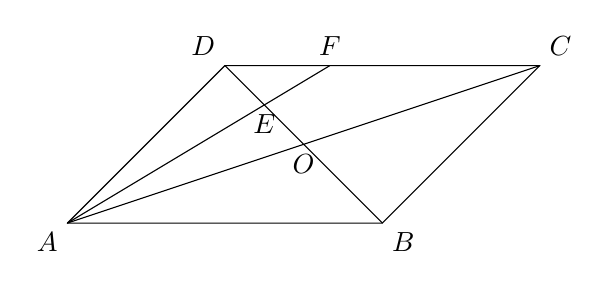
\begin{tikzpicture}[>=stealth, line cap = round, line join = round, scale = 2]
        \draw (0,0) node [below left] {$A$} -- (2,0) node [below right] {$B$}-- (3,1) node [above right] {$C$} -- (1,1) node [above left] {$D$}-- cycle;
        \draw (0,0) -- (3,1) (2,0) -- (1,1);
        \draw (0,0) -- (5/3,1) node [above] {$F$};
        \draw (1.5,0.5) node [below] {$O$};
        \draw (1.25,0.75) node [below] {$E$};
    \end{tikzpicture}
\end{center}
\item 平面上点$ABC$满足$|\overrightarrow{AB}|=3$, $|\overrightarrow{BC}|=4$, $|\overrightarrow{CA}|=5$, 则$\overrightarrow{AB}\cdot \overrightarrow{BC}+\overrightarrow{BC}\cdot \overrightarrow{CA}+\overrightarrow{CA}\cdot \overrightarrow{AB}$=\blank{50}.
\item 在$\triangle ABC$中, $\angle A=60^\circ$, $AB=3$, $AC=2$. 若$\overrightarrow{BD}=2\overrightarrow{DC}$, $\overrightarrow{AE}=\lambda \overrightarrow{AC}-\overrightarrow{AB}$, 且$\overrightarrow{AD}\cdot \overrightarrow{AE}=-4$, 则$\lambda$的值为\blank{50}.
\item $\overrightarrow a$、$\overrightarrow b$是非零向量且满足$(\overrightarrow a-2\overrightarrow b)\perp \overrightarrow a$, $(\overrightarrow b-2\overrightarrow a)\perp \overrightarrow b$, 则$\overrightarrow a$与$\overrightarrow b$的夹角是\blank{50}.
\item (1) 已知$\overrightarrow a$与$\overrightarrow b$都是非零向量, 且$|\overrightarrow a|=|\overrightarrow b|=|\overrightarrow a-\overrightarrow b|$, 求$\overrightarrow a$与$\overrightarrow a+\overrightarrow b$的夹角;\\
(2) 已知向量$\overrightarrow a$与$\overrightarrow b$的夹角为$120^\circ$, $|\overrightarrow a|=3,|\overrightarrow a+\overrightarrow b|=\sqrt{13}$, 求$|\overrightarrow b|$的值.
\item *已知向量$\overrightarrow a$、$\overrightarrow b$满足$| \overrightarrow a|=1$, $|\overrightarrow{b}|=2$, 求$|\overrightarrow a+\overrightarrow b|+|\overrightarrow a-\overrightarrow b|$的最小值、最大值.



% 第35讲 8+3+8

\item 若$\overrightarrow{AB}=(2,4)$, $\overrightarrow{AC}=(1,3)$, 则$\overrightarrow{BC}$方向相反的单位向量是\blank{50}.
\item 已知点$P_1(2,-1)$、$P_2(0,5)$, 若点$P$在直线$P_1P_2$上, 且满足$|\overrightarrow{P_1P_2}|=2|\overrightarrow{PP_2}|$, 则点$P$的坐标为\blank{50}.
\item 若三点$A(2,2)$、$B(a,0)$、$C(0,4)$共线, 则$a$的值等于\blank{50}.
\item 已知$\overrightarrow{e_1},\overrightarrow{e_2}$是不平行的向量, 设$\overrightarrow a=\overrightarrow {e_1}+k\overrightarrow {e_2}$, $\overrightarrow b=k\overrightarrow {e_1}+\overrightarrow {e_2}$, 则$\overrightarrow a$与$\overrightarrow b$平行的充要条件是实数$k$等于\blank{50}.
\item 已知向量$\overrightarrow a=(1,2)$, $\overrightarrow b=(0,3)$, 则与$\overrightarrow a$垂直的单位向量的坐标为\blank{50}; $\overrightarrow b$在$\overrightarrow a$的方向上的投影为\blank{50}.
\item 已知$\triangle ABC$的三个顶点分别是$A(1,\dfrac 32)$, $B(4,-2)$, $C(1,y)$, 其重心坐标为$G(x,-1)$, 则$x,y$的值分别是
\blank{50}.
\item 若$\overrightarrow a=(x,1)$, $\overrightarrow b=(2,3x)$, 那么$\dfrac{\overrightarrow a\cdot \overrightarrow b}{| \overrightarrow a|^2}+{|\overrightarrow b |^2}$的取值范围为\blank{50}.
\item 设向量$\overrightarrow{OA}=(1,-2)$, $\overrightarrow{OB}=(a,-1)$, $\overrightarrow{OC}=(-b,0)$, 其中点$O$为坐标原点, $a>0$, $b>0$, 若$A$、$B$、$C$三点共线, 则$\dfrac 1a+\dfrac 2b$的最小值为\blank{50}.
\item 已知直线$l$上两个点$A(0,3)$、$C(3,0)$, $O$为坐标原点.\\
(1) 若$\overrightarrow{OD}=-\dfrac 13\overrightarrow{OA}+\dfrac 43\overrightarrow{OC}$, 试确定点$D$与直线$l$的位置关系;\\
(2) 已知点$B(1,2)$是直线$l$上的一点, 求证: 若存在实数$m,n$使向量$\overrightarrow{OB}=m\cdot \overrightarrow{OA}+n\cdot \overrightarrow{OC}$, 则 $m+n=1$;\\
(3) 若存在实数$m,n$使向量$\overrightarrow{OB}=m\overrightarrow{OA}+n\overrightarrow{OC}$, 且$m+n=2$, 写出满足条件的所有点$B$的轨迹.
\item 已知$\overrightarrow m=(2\sqrt 3,1)$, $\overrightarrow n=(\cos^2\dfrac A2,\sin A)$, $A$、$B$、$C$是$\triangle ABC$的内角.\\
(1) 当$A=\dfrac{\pi}2$时, 求$|\overrightarrow n|$的值;\\
(2) 若$C=\dfrac{2\pi}3$, $|AB|=3$, 当$\overrightarrow m\cdot\overrightarrow n$取最大值时, 求$A$的大小及边$BC$的长.
\item 已知$\triangle ABC$的顶点坐标分别为$A(1,0)$, $B(5,8)$, $C(7,-4)$, 在边$AB$上有一点$P$, 其横坐标为$4$, 在边$AC$上求一点$Q$, 使线段$PQ$把$\triangle ABC$分成面积相等的两个部分.
\item 给出下列命题:\\
\textcircled{1} 非零向量$\overrightarrow a$、$\overrightarrow b$满足$|\overrightarrow a|=|\overrightarrow b|=|\overrightarrow a-\overrightarrow b|$, 则$\overrightarrow a$与$\overrightarrow a+\overrightarrow b$的夹角为$30^\circ$;\\
\textcircled{2} $\overrightarrow b\cdot \overrightarrow b>0$, 是$\overrightarrow a$、$\overrightarrow b$的夹角为锐角的充要条件;\\
\textcircled{3}  将函数$y=|x-1|$的图像按向量$\overrightarrow a=(-1,0)$平移, 得到的图像对应的函数表达式为$y=|x|$;\\
\textcircled{4} 在$\triangle ABC$中, 若$(\overrightarrow{AB}+\overrightarrow{AC})\cdot (\overrightarrow{AB}-\overrightarrow{AC})=0$, 则$\triangle ABC$为等腰三角形.\\
以上命题正确的是\blank{50}(注: 把你认为正确的命题的序号都填上).
\item 若$\overrightarrow a$和$\overrightarrow b$夹角为$120^\circ$, 且$|\overrightarrow a|=|\overrightarrow b|=1$, $| \overrightarrow c|=2$, $\overrightarrow c$与$\overrightarrow a$、$\overrightarrow b$夹角均为$60^\circ$, 用$\overrightarrow a$和$\overrightarrow b$表示$\overrightarrow c$为\blank{50}.
\item 在平面直角坐标系中, 已知$A(1,0)$、$B(0,-1)$, $P$是曲线$y=\sqrt{1-x^2}$上一个动点, 则$\overrightarrow{BP}\cdot \overrightarrow{BA}$的取值范围是\blank{50}.
\item 设$\overrightarrow{PA}=(k,12)$, $\overrightarrow{PB}=(4,5)$, $\overrightarrow{PC}=(10,k)$, 则$k=$\blank{50}时, 点$A$、$B$、$C$共线.
\item 已知直角梯形$ABCD$ , $AD\parallel BC$, $\angle BAD=90^\circ$. $AD=2$, $BC=1$, $P$是腰$AB$上的动点, 则$|\overrightarrow{PC}+\overrightarrow{PD}|$的最小值为\blank{50}.
\item 已知三角形$ABC$, $\overrightarrow{AB}=(k-1,2)$, $\overrightarrow{AC}=(-1,2)$.\\
(1) 若$k=4$, 求$S_{\triangle ABC}$; (2)若三角形为直角三角形, 求$S_{\triangle ABC}$.
\item 已知平面内三点$P(-2,0)$, $Q(-1,1)$和$R(-3,0)$, 设$\overrightarrow m=\overrightarrow{PQ}$, $\overrightarrow n=\overrightarrow{PR}$, 当实数$k$为何值时, 向量$k\overrightarrow m+\overrightarrow n$与向量$k\overrightarrow m-2\overrightarrow n$互相垂直、平行?
\item 在矩形$ABCD$中, $AB=1$, $AD=2$, 动点$P$在以点$C$为圆心且与$BD$相切的圆上. 若$\overrightarrow{AP}=\lambda \overrightarrow{AB}+\mu \overrightarrow{AD}$, 求$\lambda +\mu$的最大值.


% 第36讲 8+3+8

\item 直线$bx+ay=ab$($a<0,\ b<0$)的倾斜角为\blank{50}.
\item 过原点、且倾斜角为直线$y=\dfrac 12x-3$的倾斜角两倍的直线方程为\blank{50}.
\item $f(x)=a\sin x-b\cos x$($ab\ne 0$)的一条对称轴方程是$x=\dfrac{\pi}4$, 则直线$ax-by+c=0$的倾斜角为\blank{50}.
\item 若$\triangle ABC$顶点的坐标分别为$A(2,3)$, $B(-1,4)$, $C(0,-3)$, 则$BC$边上的高所在的直线的方程是\blank{50}, $BC$边的中线所在的直线的方程是\blank{50}.
\item (1) 已知直线$l_1:(a+3)x+(2a+5)y-3=0$和$l_2:(1-2a)x+(a-3)y+4=0$, 若$l_1$的方向向量是$l_2$的法向量, 则$a$的值为\blank{50};\\
(2)若直线$l_1:mx+2y+6=0$和直线$l_2:x+(m-1)y+m^2-1=0$平行, 则实数$m$的值为\blank{50}.
\item 已知直线$l:5x+2y+3=0$.\\
(1) 直线$l_1:3x+7y-13=0$与$l$所成的角的大小为\blank{50};\\
(2) 若$l_2$经过点$P(2,1)$、且与$l$的夹角等于$\dfrac{\pi}4$, 则直线$l_2$的方程为\blank{50}.
\item 过点$P(1,2)$作直线$l$, 使它到两点$A(2,3)$、$B(4,-5)$的距离相等, 则直线$l$的方程为\blank{50}.
\item (1) 点$P(-2,-1)$关于直线$l:x+2y-2=0$的对称点$Q$的坐标为\blank{50};\\
(2) 直线$l_1:y=2x+3$关于直线$l:y=x+1$对称的直线$l_2$的方程为\blank{50}.
\item 直线$l$过点$M(-1,2)$且与以$A(-2,-3)$、$B(3,0)$为端点的线段(含端点)有公共点.\\
(1) 求直线$l$的倾斜角$\alpha$的取值范围;\\
(2) 若直线$l$的斜率存在, 求其斜率$k$的取值范围.
\item 已知点$A(4,1)$、$B(6,-3)$, 在$x$轴上求一点$M$, 使
(1) $|MA|^2+|MB|^2$最小;\\
(2) $|MA|+|MB|$最小;\\
(3) $||MA|-|MB||$最小;\\
(4) $|MB|-|MA|$最大.
\item (1) 求过点$P(1,2)$且在两坐标轴上截距相等的直线方程;\\
(2) 求过点$P(1,2)$并且在两坐标轴上的截距的绝对值相等的直线方程;\\
(3) 直线过点$P(1,2)$分别与$x$轴和$y$轴的正半轴交于$A$、$B$两点, 求使$\triangle OAB$面积最小的直线方程.
\item 直线$x-y\cos \theta +1=0$的倾斜角$\alpha$的范围是\blank{50}.
\item 写出满足下列条件的直线方程:\\
(1) 过点$(1,-1)$, 且倾斜角为$\alpha=\pi-\arctan\dfrac 12$:\blank{50};\\
(2) 过点$(2,3)$与$(-1,-2)$:\blank{50};\\
(3) 过点$(2,3)$、方向向量为$\overrightarrow d=(4,7)$的直线方程是\blank{50};\\
(4) 过点$(2,3)$、法向量$\overrightarrow{n}=(8,9)$的直线方程是\blank{50};\\
(5) 已知直线$l$过直线$l_1:3x-5y-10=0$和$l_2:x+y+1=0$的交点, 且平行于$l_3:x+2y-5=0$, 则直线$l$的方程为\blank{50}.
\item 已知两直线$l_1:x+m^2y+6=0$与$l_2:(m-2)x+3my+2m=0$. 若$l_1$、$l_2$相交, 则$m$的取值范围为\blank{50}; 若$l_1$、$l_2$平行, 则$m$的值为\blank{50}; 若$l_1$、$l_2$重合, 则$m$的值为\blank{50}.
\item (1) 点$P(-1,-1)$到直线$l:2x-3y-11=0$的距离$d$的值是\blank{50};\\
(2) 直线$x=3$与直线$2x-y+3=0$的夹角是\blank{50};\\
(3) 直线$l$过点$P(-4,1)$, 且与直线$m:3x-y+1=0$的夹角大小为$\arccos\dfrac{3\sqrt{10}}{10}$, 则$l$的方程是\blank{50}.
\item (1) 点$P(-2,-1)$关于直线$x+y-2=0$的对称点的坐标是\blank{50};\\
(2) 直线$l:x+2y-11=0$关于点$(-1,1)$对称的直线方程是\blank{50};\\
(3) 直线$m:3x-2y-6=0$关于直线$l:2x-3y+1=0$对称的直线方程是\blank{50}.
\item 将直线$l_1:nx+y-n=0$、$l_2:x+ny-n=0$($n\in \mathbf{N}^*$)、$x$轴、$y$轴围成的封闭区域的面积记为$S_n$, 则$\displaystyle\lim_{n\to \infty}S_n=$\blank{50}.
\item 已知实数$x_1,x_2,y_1,y_2$满足: $x_1^2+y_1^2=1$, $x_2^2+y_2^2=1$, $x_1x_2+y_1y_2=\dfrac 12$, 则$\dfrac{|x_1+y_1-1|}{\sqrt 2}+\dfrac{|x_2+y_2-1|}{\sqrt 2}$的最大值为\blank{50}.
\item 如图, 用$35$个单位正方形拼成一个矩形, 点$P_1$、$P_2$、$P_3$、$P_4$以及四个标记为``
\begin{tikzpicture} \filldraw ({-0.0625*sqrt(3)},-0.0625) -- ({0.0625*sqrt(3)},-0.0625) -- (0,0.125) -- cycle; \end{tikzpicture}''的点在正方形的顶点处, 设集合$\Omega =\{P_1,P_2,P_3,P_4\}$, 点$P\in \Omega$, 过$P$作直线$l_P$, 使得不在$l_P$上的``
\begin{tikzpicture} \filldraw ({-0.0625*sqrt(3)},-0.0625) -- ({0.0625*sqrt(3)},-0.0625) -- (0,0.125) -- cycle; \end{tikzpicture}''的点分布在$l_P$的两侧. 用$D_1(l_P)$和$D_2(l_P)$分别表示$l_P$一侧和另一侧的``
\begin{tikzpicture} \filldraw ({-0.0625*sqrt(3)},-0.0625) -- ({0.0625*sqrt(3)},-0.0625) -- (0,0.125) -- cycle; \end{tikzpicture}''的点到$l_P$的距离之和. 若过$P$的直线$l_P$中有且只有一条满足$D_1(l_P)=D_2(l_P)$, 则$\Omega$中所有这样的$P$为\blank{50}.
\begin{center}
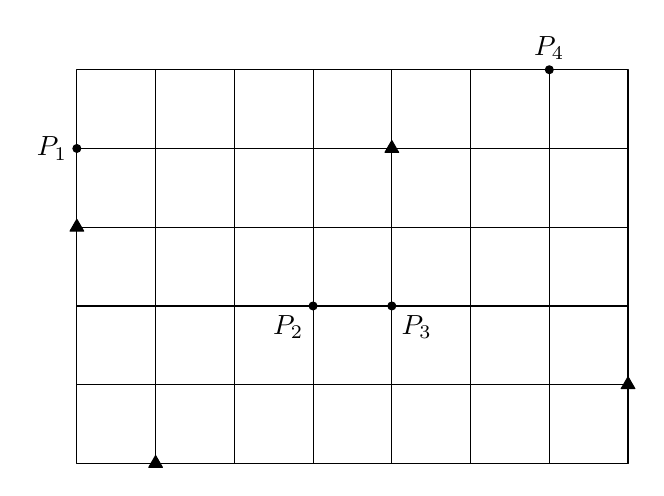
\begin{tikzpicture}[>=latex, line cap = round, line join = round]
    \foreach \i in {0,1,...,7}
        \draw (\i,0) -- (\i,5);
    \foreach \i in {0,1,...,5}
        \draw (0,\i) -- (7,\i);
    \filldraw (0,4) circle (0.05) node [left] {$P_1$};
    \filldraw (3,2) circle (0.05) node [below left] {$P_2$};
    \filldraw (4,2) circle (0.05) node [below right] {$P_3$};
    \filldraw (6,5) circle (0.05) node [above] {$P_4$};
    \filldraw (1,0) ++ (210:0.1) --++ ({0.1*sqrt(3)},0) --++ (120:{0.1*sqrt(3)}) -- cycle;
    \filldraw (0,3) ++ (210:0.1) --++ ({0.1*sqrt(3)},0) --++ (120:{0.1*sqrt(3)}) -- cycle;
    \filldraw (4,4) ++ (210:0.1) --++ ({0.1*sqrt(3)},0) --++ (120:{0.1*sqrt(3)}) -- cycle;
    \filldraw (7,1) ++ (210:0.1) --++ ({0.1*sqrt(3)},0) --++ (120:{0.1*sqrt(3)}) -- cycle;
\end{tikzpicture}
\end{center}


% 第37讲 8+3+7

\item 已知三点$A(2,-3)$、$B(-2,-5)$, 求分别满足下列条件的圆方程:\\
(1) 以$A$、$B$两点为直径的圆为\blank{50};\\
(2) 过$A$、$B$两点, 且圆心在直线$x-2y-3=0$上的圆为\blank{50}.
\item 若方程$x^2+y^2+ax+2ay+2a^2+a-1=0$表示圆, 则$a$的取值范围是\blank{50}.
\item (1) 过点$(3,4)$作圆$x^2+y^2=25$的切线$l$, 则$l$的方程为\blank{50};\\
(2) 过点$(2,4)$作圆$x^2+y^2-2x=0$的切线$m$, 则$m$的方程为\blank{50}.
\item 若点$P$在圆$x^2+y^2+4x-6y+12=0$上运动, 点$Q$在直线$4x+3y=21$上运动, 则$|PQ|$的最小值是\blank{50}.
\item 已知圆$x^2+y^2=8$内一点$P(-1,2)$, 过点$P$作直线$l$交圆于$A$、$B$, 若弦$AB$恰被点$P$平分, 则直线$l$的方程为\blank{50}.
\item 若直线$ax+by=1$与圆$C:x^2+y^2=1$相交, 则点$P(a,b)$与圆$C$的位置关系是\bracket{20}.
\twoch{点在圆内}{点在圆上}{点在圆外}{随$a,b$取值的变化而变化}
\item 若关于$x$的方程$x+\sqrt{4-x^2}=m$有且仅有一个实数解, 则实数$m$的取值范围是\blank{50}.
\item 设$f(x,y)=ax+by+c$, 其中$a,b$不全为零. 给定直线$l:f(x,y)=0$及其外一点$P(x_0,y_0)$, 直线$m:f(x,y)-f(x_0,y_0)=0$, 则\bracket{20}
\twoch{点$P$在直线$m$上, 直线$m$与$l$平行}{点$P$在直线$m$上, 直线$m$与$l$不平行}{点$P$在直线$m$外, 直线$m$与$l$平行}{点$P$在直线$m$外, 直线$m$与$l$不平行}
\item 已知圆$C:x^2+y^2-4x-14y+45=0$及点$Q(-2,3)$.\\
(1) 若$P(m,m+1)$在圆$C$上, 求线段$PQ$的长及直线$PQ$的斜率;\\
(2) 若$P$为圆$C$上任意一点, 求线段$PQ$的长的最大值和最小值;\\
(3) 若点$M(a,b)$在圆$C$上, 求$u=\dfrac{b-3}{a+2}$的最大值和最小值.
\item 过原点的直线与圆$x^2+y^2-6x+5=0$相交于$A$、$B$两点, 求弦$AB$的中点$M$的轨迹方程.
\item 已知圆$C:x^2+y^2=25$, 过定点$P(-4,0)$的直线$l$交圆$C$于$A$、$B$两点.\\
(1) 若直线$l$的斜率为$1$, 求弦长$|AB|$;\\
(2) 求弦长$|AB|$的取值范围;\\
(3) 求$\triangle AOB$面积的取值范围.
\item 圆$x^2+y^2-2x-4y-1=0$关于直线$x-y+3=0$的对称的曲线的方程为\blank{50}.
\item 若直线$mx+ny-3=0$与圆$x^2+y^2=3$没有公共点, 则$m^2+n^2$的取值范围为\blank{50}.
\item 方程$|x|-1=\sqrt{1-y^2}$表示的曲线是\bracket{20}.
\twoch{一条直线}{两条射线}{一个圆}{两个半圆(即两段圆弧)}\item 求满足下列条件的圆的方程:\\
(1) 经过点$(2,-1)$且和直线$x-y=1$相切, 同时圆心在直线$y=-2x$上的圆的方程为\blank{50};\\
(2) 经过点$A(-2,-4)$, 且与直线$l:x+3y-26=0$相切于点$B(8,6)$的圆的方程为\blank{50}.
\item 已知方程$x^2+y^2+Dx+Ey+F=0$表示一个圆. ``$D^2=4F$''是``该圆与$x$轴相切''的\bracket{20}条件.
\fourch{充分非必要}{必要非充分}{充要}{既非充分又非必要}\item 圆$x^2+y^2=4$与$x$轴相交于$A$、$B$两点, 圆内的动点$P$使$|PA|$, $|PO|$, $|PB|$成等比数列, 求$\overrightarrow{PA}\cdot \overrightarrow{PB}$的取值范围.
\item 已知$m\in \mathbf{R}$, 直线$l:mx-(m^2+1)y=4m$和圆$C:x^2+y^2-8x+4y+16=0$.\\
(1) 求直线$l$的斜率$k$的取值范围;\\
(2) 直线$l$能否将圆$C$分割成弧长的比值为$\dfrac{1}{2}$的两段圆弧? 为什么?


% 第38讲 8+3+8

\item 若点$P(-3,0)$是椭圆$x^2+2y^2-k=0$上的点, 则椭圆的焦点坐标是\blank{50}.
\item 方程$\dfrac{x^2}{k-5}+\dfrac{y^2}{3-k}=-1$表示焦点在$y$轴上的椭圆, 则实数$k$的取值范围是\blank{50}.
\item (1) 焦距是$2\sqrt 5$, 长轴长是$8$的椭圆的标准方程是\blank{50};\\
(2) 长轴长是短轴长的2倍, 且经过点$(2,1)$的椭圆的标准方程是\blank{50};\\
(3) 经过点$A(\sqrt 3,-2)$、$B(\sqrt 5,\dfrac{\sqrt{30}}3)$的椭圆的方程是\blank{50}.
\item 已知点$P$是椭圆$\dfrac{x^2}{25}+\dfrac{y^2}9=1$上一点, $F_1F_2$是焦点, 若$\angle F_1PF_2=60^\circ$, 则三角形$F_1PF_2$的面积为\blank{50}.
\item 已知椭圆$\dfrac{x^2}{36}+\dfrac{y^2}{16}$=1的弦过点$P(3,2)$且被$P$平分, 则此弦所在的直线方程为\blank{50}.
\item 椭圆$\dfrac{x^2}{45}+\dfrac{y^2}{20}=1$的焦点为$F_1$、$F_2$, 过原点$O$作直线交椭圆于$A$、$B$两点, 若$\triangle ABF_2$的面积为$20$, 则点$A$的纵坐标为\blank{50}.
\item 若曲线$\dfrac{x^2}2+y^2=1 \ (y\ge 0)$与$y=x+m$有两个公共点, 则实数$m$的取值范围为\blank{50}.
\item 已知椭圆$\dfrac{x^2}m+\dfrac{y^2}6=1$, $F_1,F_2$是它的两个焦点, 若椭圆上存在两个不同的点$P$, 使$\angle F_1PF_2=90^\circ$, 则$m=$\blank{50}.
\item 已知椭圆$\dfrac{y^2}9+{x^2}=1$, 一条不与坐标轴平行的直线$l$与该椭圆交于不同的两点$M$、$N$, 且线段$MN$的中点的横坐标为$-\dfrac 12$.\\
(1) 求直线$l$的斜率的取值范围;\\
(2) 求直线$l$的倾斜角的取值范围.
\item 已知椭圆$\dfrac{x^2}2+{y^2}=1$.\\
(1) *过椭圆的左焦点$F$引椭圆的割线, 求截得的弦的中点$P$的轨迹方程;\\
(2) 求斜率为2的平行弦中点$Q$的轨迹方程;\\
(3) 求过点$M(\dfrac 12,\dfrac 12)$且被$M$平分的弦所在直线方程.
\item 设椭圆$C:\dfrac{x^2}2+{y^2}=1$的右焦点为$F$, 过$F$的直线$l$与$C$交于$AB$两点, 点$M$的坐标为$(2,0)$.\\
(1) 当$l$与$x$轴垂直时, 求直线$AM$的方程;\\
(2) 设$O$为坐标原点, 证明: $\angle OMA=\angle OMB$.
\item 若椭圆的中心为原点, 焦点在坐标轴上, 焦点到长轴端点的距离分别为$\sqrt 2-1$与$\sqrt 2+1$, 则椭圆的方程为\blank{50}.
\item 与椭圆$\dfrac{x^2}9+\dfrac{y^2}4=1$有相同的焦点, 且经过点$(3,-2)$的椭圆为\blank{50}.
\item 已知圆$A:(x-4)^2+y^2=100$, 圆$B:(x+4)^2+y^2=1$, 动圆P与圆$A$内切且与圆$B$外切, 则点P的轨迹方程是\blank{50}.
\item 椭圆${x^2}+\dfrac{y^2}4=1$上的点$P(x,y)$到定直线$x+y-6=0$的最远距离是\blank{50}.
\item 记椭圆$\dfrac{x^2}4+\dfrac{n{y^2}}{4n+1}=1$围成的区域(含边界)为$\Omega_n \ (n=1,2,\cdots)$, 当点$(x,y)$分别在$\Omega_1,\Omega_2,\cdots$上时, $x+y$的最大值分别是$M_1,M_2,\cdots$, 则$\displaystyle\lim_{n\to \infty}M_n=$\blank{50}.
\item 椭圆$\dfrac{x^2}9+\dfrac{y^2}4=1$上的动点$P(x,y)$与定点$M(m,0)$($0<m<3$)的距离的最小值为$1$, 求$m$的值.
\item 在平面直角坐标系$xOy$中, 经过点$(0,\sqrt 2)$且斜率为$k$的直线$l$与椭圆$\dfrac{x^2}2+y^2=1$有两个不同的交点$P$、$Q$.\\
(1) 求$k$的取值范围;\\
(2) 设椭圆与$x$轴正半轴、$y$轴正半轴的交点分别为$A$、$B$. 问是否存在常数$k$, 使得向量$\overrightarrow{OP}+\overrightarrow{OQ}$与$\overrightarrow{AB}$共线? 如果存在, 求出$k$的值; 如果不存在, 说明理由.
\item *在平面直角坐标系$xOy$中, 已知椭圆$\Gamma:\dfrac{x^2}4+{y^2}=1$, $A$为$\Gamma$的上顶点, $P$为$\Gamma$上异于上、下顶点的动点, $M$为正半轴上的动点.\\
(1) 若$P$在第一象限, 且$|OP|=\sqrt 2$, 求$P$的坐标;\\
(2) 设$P(\dfrac 85,\dfrac 35)$, 若以$A$、$P$、$M$为顶点的三角形是直角三角形, 求$M$的横坐标$m$;\\
(3) 若$|MA|=|MP|$, 直线$AQ$与$\Gamma$交于另一点$C$, 且$\overrightarrow{AQ}=2\overrightarrow{AC}$, $\overrightarrow{PQ}=4\overrightarrow{PM}$, 求直线$AQ$的方程.


% 第39讲 8+3+8

\item 已知双曲线的中心在原点, 焦点在坐标轴上. 分别求满足下列条件的双曲线的标准方程:\\
(1) 以椭圆$\dfrac{x^2}{25}+\dfrac{y^2}9=1$的长轴顶点为焦点, 且过$P(4\sqrt 2,3)$的双曲线方程为\blank{50};\\
(2) 点$P(\sqrt 2,1)$在双曲线上, 且它到双曲线的右焦点的距离是$1$, 该双曲线方程为\blank{50}.
\item 双曲线顶点间距离为$6$, 渐近线方程为$y=\pm \dfrac 32x$, 该双曲线方程为\blank{50}.
\item 双曲线$4x^2+ky^2-4k=0$的虚轴长为\blank{50}.
\item 双曲线$\dfrac{x^2}4-\dfrac{y^2}8=1$的两条渐近线所夹的锐角的大小为\blank{50}.
\item 已知$F_1$、$F_2$是双曲线$\dfrac{x^2}{16}-\dfrac{y^2}{20}=1$的焦点, 点$P$在双曲线上. 若$|PF_1|=9$, 则$|PF_2|=$\blank{50}.
\item 直线$y=kx+2$与双曲线$x^2-y^2=6$的右支交于不同的两点, 则$k$的取值范围为\blank{50}.
\item 已知动圆$M$与圆$C_1:(x+4)^2+y^2=2$, 与圆$C_2:(x-4)^2+y^2=2$相内切, 则动圆圆心$M$的轨迹方程为\blank{50}.
\item 已知两点$M(-5,0)$, $N(5,0)$. 在下列直线上, 存在点$P$满足$|MP|-|NP|=6$的所有直线方程是\blank{50}(填写序号).\\ \textcircled{1} $y=\dfrac 53(x+2)$; \textcircled{2} $y=\dfrac 53(x-5)$; \textcircled{3} $y=x-2$; \textcircled{4} $y=4(x+2)$.
\item 已知双曲线$C$的一个顶点$A(0,\sqrt 2)$, 其渐近线经过原点且与圆$M:(x-\sqrt 2)^2+y^2=1$相切.\\
(1) 求双曲线$C$的方程;\\
(2) 已知直线$l:y=x-\sqrt 2$, 在双曲线的上支求点$P$, 使点$P$与直线$l$的距离等于$\sqrt 2$.
\item 在双曲线$\dfrac{y^2}{12}-\dfrac{x^2}{13}=1$上支上有不同三点$A(x_1,y_1)$、$B(\sqrt{26},6)$、$C(x_2,y_2)$到焦点$F(0,5)$的距离成等差数列.\\
(1) 求$y_1+y_2$的值;\\
(2) 证明: 线段$AC$的垂直平分线经过一个定点$T$并且求出这个点$T$的坐标.
\item 若椭圆$\dfrac{x^2}{m^2}+\dfrac{y^2}{n^2}=1$($m>n>0$)和双曲线$\dfrac{x^2}{a^2}-\dfrac{y^2}{b^2}=1$($a>0$, $b>0$)有相同的焦点$F_1,F_2$, 点$P$是椭圆和双曲线的一个交点.\\
(1) 求证: $|PF_1|\cdot |PF_2|=m^2-a^2$;\\
(2) 求证: $\triangle PF_1F_2$的面积$S=nb$.
\item 若双曲线$8mx^2-my^2=8$的一个焦点是$(0,3)$, 则$m=$\blank{50};
\item 和双曲线$\dfrac{x^2}9-\dfrac{y^2}{16}=1$有共同的渐近线, 并且实轴长为$12$的双曲线方程是\blank{50};
\item 过$P(1,0)$作直线$l$与双曲线${x^2}-\dfrac{y^2}4=1$只有一个公共点, 则这样的直线共有\blank{50}条.
\item 已知双曲线$\dfrac{x^2}{12}-\dfrac{y^2}4=1$的右焦点为$F$, 若过点$F$的直线$l$与双曲线的右支有且只有一个公共点, 则直线$l$的斜率的取值范围为\blank{50}.
\item 若关于$x$的方程$\sqrt{x^2-1}=x+m$没有实数解, 则实数$m$的取值范围是\blank{50};
\item 求渐近线为$3x\pm 4y=0$, 焦点为椭圆$\dfrac{x^2}{10}+\dfrac{y^2}5=1$的一对顶点的双曲线方程.
\item 已知$F_1F_2$是双曲线${x^2}-\dfrac{y^2}{b^2}=1$($b>0$)的左、右焦点, 直线$l$过$F_2$且与双曲线交于$AB$两点.\\
(1) 若$l$的倾斜角为$\dfrac{\pi}2$, $\triangle F_1AB$是等边三角形, 求双曲线的渐近线方程;\\
(2) 设$b=\sqrt 3$, 若$l$的斜率存在, 且$(\overrightarrow{F_1A}+\overrightarrow{F_1B})\cdot \overrightarrow{AB}=0$, 求$l$的斜率.
\item 设双曲线${x^2}-\dfrac{y^2}4=1$的右顶点为$A$, 定点$B$的坐标为$(\dfrac 12,1)$.\\
(1) 是否存在过$B(\dfrac 12,1)$点且被点$B$平分的双曲线的弦$PQ$, 若存在求出弦$PQ$所在直线方程, 若不存在说明理由;\\
(2) 过点$B$的动直线$l$交双曲线于$P,Q$两点, $M$为线段$PQ$的中点, 求直线$AM$的斜率的取值范围.



% 第40讲 8+3+7

\item 已知抛物线的顶点在原点, 焦点在坐标轴上. 分别求适合下列条件的抛物线的标准方程:\\
(1) 过点$(-2,3)$的抛物线为\blank{50};\\
(2) 准线过点$(2,3)$的抛物线为\blank{50};\\
(3) 焦点在直线$3x-4y-12=0$上的抛物线为\blank{50};\\
(4) 焦点在$y$轴上, 抛物线上一点$M(m,-3)$到焦点的距离等于$5$的抛物线为\blank{50}.
\item 过点$(2,1)$与抛物线$y=x^2$恰有一个公共点的直线有\blank{50}条.
\item 抛物线$y=x^2$上到直线$2x-y=4$距离最短的点的坐标为\blank{50}.
\item 已知点$A(3,4)$, $F$是抛物线$y^2=8x$的焦点, $M$是抛物线上的动点.当$|MA|+|MF|$最小时, $M$的坐标是\blank{50}.
\item 若$AB$是抛物线$y=x^2$的一条过焦点的弦, 且$|AB|=4$, 则$AB$的中点到直线$y+1=0$的距离是\blank{50}.
\item 一动点到定点$A(0,2)$的距离比定直线$y=-3$的距离小$1$, 则动点的轨迹方程是\blank{50}.
\item 已知$F$是抛物线$C:y^2=4x$的焦点, $AB$是抛物线$C$上的两个点, 线段$AB$的中点为$M(2,2)$, 则$\triangle ABF$的面积等于\blank{50}.
\item 已知$A,B$是抛物线$y^2=2px(p>0)$上的两个点, $O$为坐标原点, 若$|OA|=|OB|$, 且抛物线的焦点恰为$\triangle AOB$的垂心, 则直线$AB$的方程是\blank{50}.
\item 已知点$M$到点$F(1,0)$和直线$x=3$的距离之和等于$4$, 设点$M$的轨迹为曲线$\Gamma$.\\
(1) 求曲线$\Gamma$的方程;\\
(2) 过点$F$作倾斜角为$\dfrac{\pi}4$的直线交曲线$\Gamma$于$A$、$B$两点, 求$|AB|$的值.
\item 如图, $M$是抛物线上$y^2=x$上的一点(异于原点), 动弦$ME$、$MF$分别交$x$轴于$AB$两点, 且$MA=MB$.\\
(1) 若$M$为定点, 证明: 直线$EF$的斜率为定值;\\
(2) 若$M$为动点, 且$\angle EMF={90}^{\circ}$, 求$\triangle EMF$的重心$G$的轨迹.
\begin{center}
\begin{tikzpicture}[>=latex, line cap = round, line join = round, scale = 1.5]
    \draw [->] (-0.5,0) -- (4,0) node [below] {$x$};
    \draw [->] (0,-2) -- (0,2) node [left] {$y$};
    \draw (0,0) node [below left] {$O$};    
    \draw [domain = -1.8:1.8, samples = 1000] plot (\x*\x, \x);
    \draw (1.44,1.2) node [above] {$M$};
    \draw (0.49,-0.7) node [below] {$E$} -- (1.44,1.2) -- (2.89,-1.7) node [below] {$F$} -- cycle;
    \draw (0.84,0) node [below right] {$A$} (2.04,0) node [above right] {$B$};
\end{tikzpicture}
\end{center}
\item 求证: 抛物线的准线上任意一点引抛物线的两切线互相垂直并且切点弦过定点.
\item 抛物线$y=-4x^2$的焦点坐标是\blank{50}.
\item 抛物线的焦点在双曲线$\dfrac{x^2}{25}-\dfrac{y^2}4=1$上, 则抛物线的标准方程\blank{50}.
3.点$A(-4,2)$是抛物线$y^2=-8x$内一点, 抛物线上的点$M$到$A$点的距离与它到焦点的距离之和最小, 则点$M$的坐标是\blank{50}, 最小距离是\blank{50}.
4.设$F$为抛物线$y^2=4x$的焦点, $ABC$为该抛物线上三点.若$\overrightarrow{FA}+\overrightarrow{FB}+\overrightarrow{FC}=\overrightarrow 0$, 则$|\overrightarrow{FA}|+|\overrightarrow{FB}|+|\overrightarrow{FC}|=$\blank{50}.
5.设抛物线$y^2=2x$的焦点为$F$, 过点$M(\sqrt 3,0)$的直线与抛物线相交于$AB$两点, 与抛物线的准线相交于$C$, $| BF |=2$, 则$\triangle BCF$与$\triangle ACF$的面积之比为\blank{50}.
\item 设直线$a$与抛物线$\Omega:y^2=4x$相交于不同的两点$AB$, $O$为坐标原点.\\
(1) 求抛物线$\Omega$的焦点到准线的距离;\\
(2) 若$\overrightarrow{OA}\cdot \overrightarrow{OB}=0$, 点$Q$在线段$AB$上, 满足$OQ\perp AB$, 求点$Q$的轨迹.
\item 如图, 已知点$P$是$y$轴左侧(不含$y$轴)一点, 抛物线$C:y^2=4x$上存在不同的两点$A$、$B$满足$PA$、$PB$的中点均在$C$上.\\
(1) 设$AB$中点为$M$, 证明: $PM\perp y$轴;\\
(2) 若$P$是半椭圆${x^2}+\dfrac{y^2}4=1x<0$上的动点, 求$\triangle PAB$面积的取值范围.
\begin{center}
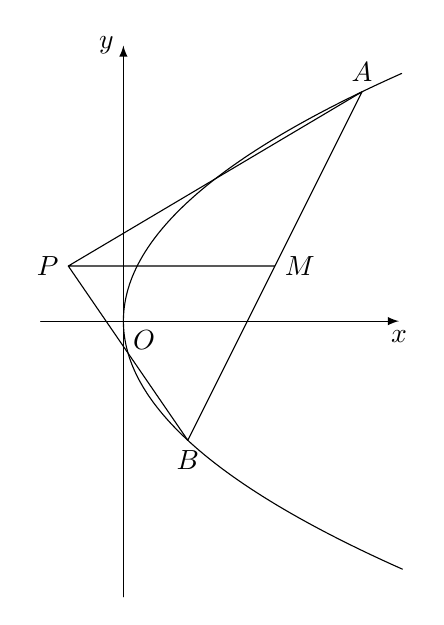
\begin{tikzpicture}[>=latex, line cap = round, line join = round, scale = 0.7]
    \draw [->] (-1.5,0) -- (5,0) node [below] {$x$};
    \draw [->] (0,-5) -- (0,5) node [left] {$y$};
    \draw (0,0) node [below right] {$O$};    
    \draw [domain = -4.5:4.5, samples = 1000] plot (\x*\x/4, \x);
    \draw ({11/4+sqrt(10)/2},{1+sqrt(10)}) node [above] {$A$} coordinate (A);
    \draw ({11/4-sqrt(10)/2},{1-sqrt(10)}) node [below] {$B$} coordinate (B);
    \draw ($(A)!0.5!0:(B)$) node [right] {$M$} coordinate (M);
    \draw (-1,1) node [left] {$P$} coordinate (P);
    \draw (P) -- (M) (A) -- (P) -- (B) -- cycle;
\end{tikzpicture}
\end{center}

% 第43讲 8+3+7

\item 下列命题中, 假命题有\blank{50}(填入序号).\\
(1) 平行于同一平面的两直线平行; (2) 平行于同一直线的两平面平行; (3) 平行于同一直线的两直线平行; (4) 平行于同一平面的两平面平行.
\item 给定空间中的直线$l$及平面$\alpha$. ``直线$l$与平面$\alpha$内无数条直线都垂直''是``直线$l$与平面$\alpha$垂直''的\blank{50}条件.
\item 对于空间三条直线$a,b,c$, 若$a\perp b$, $b\perp c$, 则$a$与$c$\bracket{20}.
\twoch{一定相交}{一定平行}{一定异面}{平行、相交、异面都有可能}
\item 如图是一个正方体的展开图. 在原正方体中, 直线$AB$与$CD$所成的角的大小为\blank{50}.
\begin{center}
    \begin{tikzpicture}[>=latex, line cap = round, line join = round, scale = 1.5]
        \draw (0,0) -- (3,0) (0,1) node [above left] {$A$} -- (4,1) (1,-1) -- (2,-1) (2,2) node [above left] {$C$} -- (4,2);
        \draw (0,0) -- (0,1) (1,-1) -- (1,1) (2,-1) -- (2,2) (3,0) -- (3,2) (4,1) -- (4,2);
        \draw (0,1) -- (1,0) node [below right] {$B$} coordinate (B) (2,2) -- (3,1) node [below right] {$D$};
        \draw [dashed] (B) --++ (45:1/2) --++ (1,0) --++ (225:1/2);
        \draw [dashed] (B) ++ (0,1) --++ (45:1/2) --++ (1,0) --++ (225:1/2);
        \draw [dashed] (B) ++ (45:1/2) --++ (0,1) ++ (1,0) --++ (0,-1);
    \end{tikzpicture}
\end{center}
\item 直线$PA$垂直于矩形$ABCD$所在的平面. 设$AP=AD=1$, $DC=2$, 则点$P$到直线$BD$的距离为\blank{50}.
\item 空间四边形$ABCD$中, 点$E,F,G$分别是边$AB,BC,CD$的中点. 若异面直线$AC$与$BD$所成的角的大小为$60^\circ$, 则$\angle EFG$的大小为\blank{50}.
\item 已知$P$是二面角$\alpha-l-\beta$内一点, 过$P$作$PA\perp \alpha$, $PB\perp \beta$, $A,B$为垂足, 若直线$PA$与$PB$所成角的大小是$80^\circ$, 则二面角$\alpha-l-\beta$的大小是\blank{50}.
\item 由一点$P$出发引三条射线$PA$, $PB$, $PC$, 若$\angle APB=45^\circ$, $\angle APC=60^\circ$, $\angle BPC=90^\circ$, 则$PA$与平面$BPC$所成角的大小是\blank{50}.
\item 如图, 在长方体$ABCD-A_1B_1C_1D_1$中, 点$E,F$分别在棱$BB_1, DD_1$上, 且$AE\perp A_1B$, $AF\perp A_1D$. 求证: $A_1C\perp$平面$AEF$.
\begin{center}
    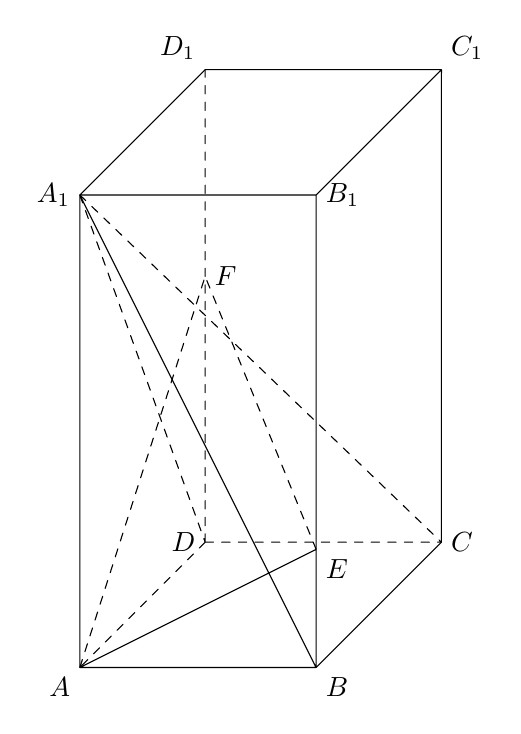
\begin{tikzpicture}[>=latex, line cap = round, line join = round, scale = 1.5]
        \draw (0,0) coordinate (A) node [below left] {$A$};
        \draw (A) ++ (2,0) coordinate (B) node [below right] {$B$};
        \draw (A) ++ (45:1.5) coordinate (D) node [left] {$D$};
        \draw (D) ++ (2,0) coordinate (C) node [right] {$C$};
        \draw (B) ++ (0,1) coordinate (E) node [below right] {$E$};
        \draw (D) ++ (0,9/4) coordinate (F) node [right] {$F$};
        \draw (A) ++ (0,4) coordinate (A1) node [left] {$A_1$};
        \draw (B) ++ (0,4) coordinate (B1) node [right] {$B_1$};
        \draw (C) ++ (0,4) coordinate (C1) node [above right] {$C_1$};
        \draw (D) ++ (0,4) coordinate (D1) node [above left] {$D_1$};
        \draw (A) -- (B) -- (C) -- (C1) -- (D1) -- (A1) -- cycle (C1) -- (B1) -- (B) (B1) -- (A1) (A1) -- (B) (A) -- (E);
        \draw [dashed] (D) -- (A) (D) -- (C) (D) -- (D1) (A1) -- (C) (A) -- (F) -- (E) (A1) -- (D);
    \end{tikzpicture}
\end{center}
\item 如图, 在棱长为$2$的正方体$ABCD-A_1B_1C_1D_1$中, $E$是$BC_1$的中点.
\begin{center}
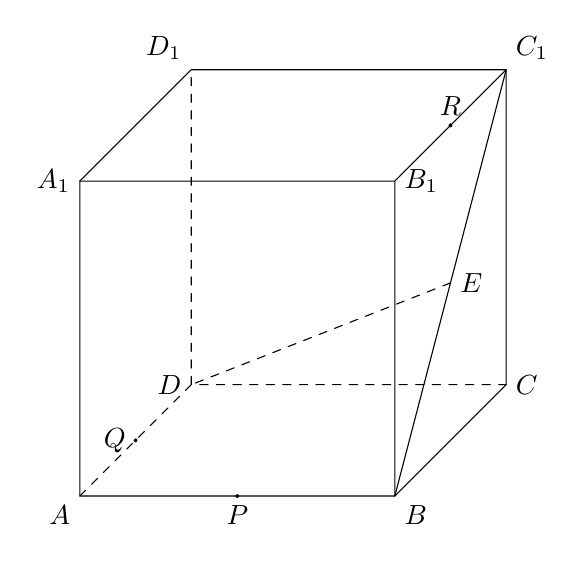
\begin{tikzpicture}[>=latex, line cap = round, line join = round]
    \draw (0,0) node [below left] {$A$} coordinate (A) -- (4,0) node [below right] {$B$} coordinate (B) --++ (45:{4/2}) node [right] {$C$} coordinate (C)
    --++ (0,4) node [above right] {$C_1$} coordinate (C1)
    --++ (-4,0) node [above left] {$D_1$} coordinate (D1) --++ (225:{4/2}) node [left] {$A_1$} coordinate (A1) -- cycle;
    \draw (4,4) node [right] {$B_1$} coordinate (B1) -- (B) (B1) --++ (45:{4/2}) (B1) --++ (-4,0);
    \draw [dashed] (0,0) --++ (45:{4/2}) node [left] {$D$} coordinate (D) --++ (4,0) (D) --++ (0,4);
    \draw (C1) -- (B);
    \draw ($(B)!0.5!0:(C1)$) node [right] {$E$} coordinate (E);
    \draw [dashed] (E) -- (D);
    \filldraw ($(A)!0.5!0:(B)$) node [below] {$P$} circle (0.02);
    \filldraw ($(A)!0.5!0:(D)$) node [left] {$Q$} circle (0.02);
    \filldraw ($(B1)!0.5!0:(C1)$) node [above] {$R$} circle (0.02);
\end{tikzpicture}
\end{center}
(1) 求直线$DE$与平面$ABCD$所成的角的大小;\\
(2) 在图中作出过点$D_1,D,E$三点的正方体$ABCD-A_1B_1C_1D_1$的截面, 并求出该截面的面积;\\
(3) $P,Q,R$分别是$AB,AD,B_1C_1$的中点, 作出过$P,Q,R$的截面.
\item 如图, $P$为三角形$ABC$所在平面外一点, $PA\perp$平面$ABC$, $\angle ABC=90^\circ$, $AE\perp PB$于$E$, $AF\perp PC$于$F$.
\begin{center}
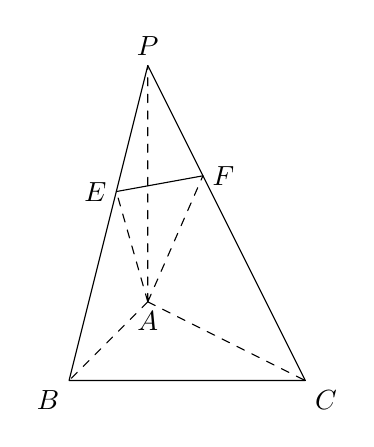
\begin{tikzpicture}[>=latex, line cap = round, line join = round]
    \draw (0,0) coordinate (B) (3,0) coordinate (C) (1,1) coordinate (A) node [below] {$A$} (1,4) coordinate (P);
    \draw (B) node [below left] {$B$} -- (C) node [below right] {$C$} -- (P) node [above] {$P$} -- cycle;
    \draw ($(B)!0.6!0:(P)$) coordinate (E) node [left] {$E$} ($(C)!0.65!0:(P)$) coordinate (F) node [right] {$F$};
    \draw (E) -- (F);
    \draw [dashed] (A) -- (P) (A) -- (B) (A) -- (C) (A) -- (E) (A) -- (F); 
\end{tikzpicture}
\end{center}
(1) 求证: $BC\perp$平面$PAB$, $AE\perp$平面$PBC$, $PC\perp$平面$AEF$;\\
(2) 若$AP=AC=2$, $\angle BPC=\theta$, 当$\theta$为何值时, 三角形$AEF$的面积$S$取到最大值? 最大值是多少?
\item 空间中有四个点, ``这四个点中恰好有三点在同一直线上''是``这四个点在同一个平面上''的\blank{50}条件;
\item 两条直线$a$、$b$满足$a\parallel b$, $b\subsetneqq \alpha$, 则$a$与平面$\alpha$的关系是\blank{50}.
\item 对于平面$M$、$N$. ``$M$内有不共线的三点到$N$的距离相等''是``$M\parallel N$''成立的\blank{50}条件;
\item 对于分别与两条异面直线都相交的两条直线, 下列结论中, 真命题有\blank{50}(填入序号).\\
(1) 一定是异面直线; (2) 不可能是平行直线; (3) 不可能是相交直线.
\item 已知$A,B$两点到平面$\alpha$的距离分别是$1$和$3$, 那么线段$AB$的中点到平面$\alpha$的距离是\blank{50}.
\item 如图, 点$P$为三棱柱$ABC-A_1B_1C_1$的侧棱$BB_1$上一点, $PM\perp BB_1$交$AA_1$于点$M$, $PN\perp BB_1$交$CC_1$于点$N$. 求证: $CC_1\perp MN$.
\begin{center}
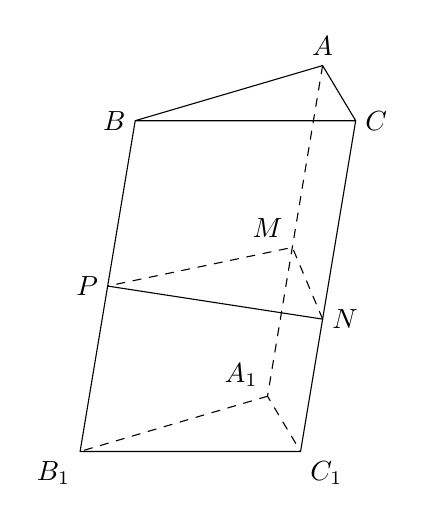
\begin{tikzpicture}[>=latex, line cap = round, line join = round, scale = 1.4]
    \draw (0,0) node [below left] {$B_1$} coordinate (B1) -- (2,0) node [below right] {$C_1$} coordinate (C1) 
    -- ++ (0.5,3) node [right] {$C$} coordinate (C) --++ (-2,0) node [left] {$B$} coordinate (B) -- cycle;
    \draw (B) --++ (1.7,0.5) node [above] {$A$} coordinate (A) -- (C);
    \draw [dashed] (A) --++ (-0.5,-3) node [above left] {$A_1$} coordinate (A1) -- (C1) (A1) -- (B1);
    \draw ($(B)!0.5!0:(B1)$) node [left] {$P$} coordinate (P);
    \draw ($(C)!0.6!0:(C1)$) node [right] {$N$} coordinate (N);
    \draw ($(A)!0.55!0:(A1)$)node [above left] {$M$} coordinate (M);
    \draw (P) -- (N);
    \draw [dashed] (N) -- (M) -- (P);
\end{tikzpicture}
\end{center}
\item 如图, 在长方体$ABCD-A'B'C'D'$中, $AB=2$, $AD=1$, $AA'=1$. 证明:\\
(1) 直线$BC'$与直线$AC$异面;\\
(2) 直线$BC'\parallel\text{平面}ACD'$, 并求$BC'$到平面$ACD'$的距离.
\begin{center}
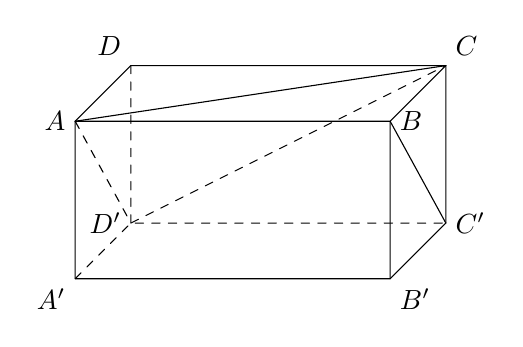
\begin{tikzpicture}[>=latex, line cap = round, line join = round, scale = 2]
    \draw (0,0) node [below left] {$A'$} coordinate (AP) --++ (2,0) node [below right] {$B'$} coordinate (BP) --++ (45:{1/2}) node [right] {$C'$} coordinate (CP)
    --++ (0,1) node [above right] {$C$} coordinate (C)
    --++ (-2,0) node [above left] {$D$} coordinate (D) --++ (225:{1/2}) node [left] {$A$} coordinate (A) -- cycle;
    \draw (AP) ++ (2,1) node [right] {$B$} coordinate (B) -- (BP) (B) --++ (45:{1/2}) (B) --++ (-2,0);
    \draw [dashed] (AP) --++ (45:{1/2}) node [left] {$D'$} coordinate (DP) --++ (2,0) (DP) --++ (0,1);
    \draw (B) -- (CP) (A) -- (C);
    \draw [dashed] (A) -- (DP) -- (C);
\end{tikzpicture}
\end{center}


% 第44讲 8+3+7

\item 下列命题中, 假命题有\blank{50}(填入序号).\\
(1) 底面是正多边形的棱锥是正棱锥; (2) 侧棱都相等的棱锥是正棱锥; (3) 有两个侧面是矩形的棱柱是直棱柱.
\item 正四棱锥底面边长为$4$, 侧棱长为$3$, 则其侧面积为\blank{50}, 其体积为\blank{50}.
\item 棱锥的高是$1$, 一个平行于底面的平面把棱锥分成体积相等的两个部分, 则顶点到这个平行于底面的平面的距离为\blank{50}.
\item 棱长为$1$的正四面体的高为\blank{50}, 体积为\blank{50}, 对棱中点的距离为\blank{50}.
\item 若两个长方体的长, 宽, 高分别为$5$, $4$, $3$, 把它们两个全等的面重合在一起组成大长方体, 则大长方体的对角线最长为\blank{50}.
\item 若一个圆柱的侧面展开图是一个正方形, 则这个圆柱的表面积与侧面积的比是\blank{50}.
\item 若圆锥的侧面展开图恰好是一个半圆, 则该圆锥的母线与底面所成的角的大小是\blank{50}.
\item 过半径为$2$的球$O$表面上一点$A$作球$O$的截面, 若$OA$与该截面所成的角的大小为$60^\circ$, 则该截面的面积是\blank{50}.
\item 如图, 圆锥的轴截面为等边三角形$SAB$, $Q$为底面圆周上一点.
\begin{center}
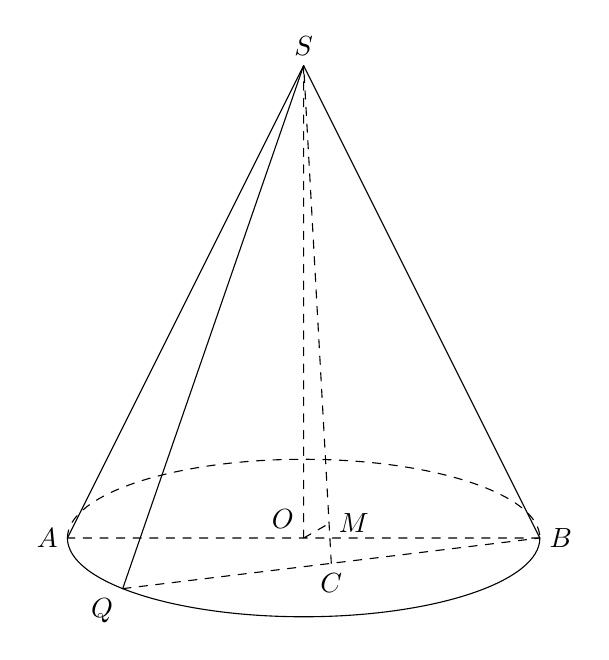
\begin{tikzpicture}[>=latex, line cap = round, line join = round, scale = 1]
    \draw (-3,0) node [left] {$A$} arc (180:360:3 and 1) node [right] {$B$} -- (0,6) coordinate (S) node [above] {$S$} -- cycle;
    \draw [dashed] (-3,0)  arc (180:0:3 and 1);
    \draw ({-3*cos(40)},{-sin(40)}) node [below left] {$Q$} coordinate (Q) -- (0,6);
    \draw [dashed] (Q) -- (3,0) coordinate (B);
    \draw [dashed] ($(Q)!0.5!0:(B)$) node [below] {$C$} coordinate (C) -- (S) -- (0,0) node [above left] {$O$} coordinate (O);
    \draw [dashed] (O) -- ($(C)!0.08!0:(S)$) node [right] {$M$} (B) -- (-3,0);
\end{tikzpicture}
\end{center}
(1) 设$C$为线段$BQ$的中点, $M$是$SC$上一点, 且$OM\perp SC$, 证明: $OM\perp\text{平面}SBQ$;\\
(2) 若$\angle AOQ=60^\circ$, $QB=2\sqrt 3$, 求圆锥的体积.
\item 取地球的半径为$6370$千米, 在北纬$45^\circ$线上, 求相隔$30^\circ$的两条经线之间的球面距离(精确到$0.1$千米).
\item 直三棱柱$ABC-A_1B_1C_1$中, 底面$ABC$为等腰直角三角形, 且$AB\perp AC$, $AB=AC=2$, $AA_1=4$, $M$是侧棱$CC_1$上一点, 设$MC=h$.\\
(1) 若$BM\perp A_1C$, 求$h$的值;\\
(2) 若直线$AM$与平面$ABC$所成的角为$\dfrac{\pi}4$, 求多面体$ABM-A_1B_1C_1$的体积.
\item 过棱锥的高的三等分点作两个平行于底面的截面, 它们将棱锥的侧面分成三部分的面积的比(自顶点开始向底面排序)为\blank{50}.
\item 已知一个凸多面体共有$9$个面, 所有棱长都为$1$, 其平面展开图如图所示, 则该凸多面体的体积为\blank{50}.
\begin{center}
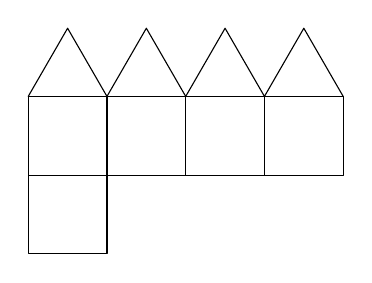
\begin{tikzpicture}[>=latex, line cap = round, line join = round, scale = 1]
    \draw (0,0) -- (4,0) -- (4,1) -- (0,1) -- cycle;
    \draw (0,0) -- (0,-1) -- (1,-1) -- (1,1) (2,1) -- (2,0) (3,1) -- (3,0);
    \draw (0,1) --++ ({1/2},{1/2*sqrt(3)}) --++ ({1/2},{-1/2*sqrt(3)}) --++ ({1/2},{1/2*sqrt(3)}) --++ ({1/2},{-1/2*sqrt(3)}) --++ ({1/2},{1/2*sqrt(3)}) --++ ({1/2},{-1/2*sqrt(3)})
    --++ ({1/2},{1/2*sqrt(3)}) --++ ({1/2},{-1/2*sqrt(3)});
\end{tikzpicture}
\end{center}
\item 若圆锥的侧面积为$20\pi$, 且母线与底面所成的角的大小为$\arccos\dfrac 45$, 则该圆锥的体积为\blank{50}.
\item 下列命题中, 假命题有\blank{50}(填入序号).\\
(1) 经过球上任意两点, 能且仅能作一个大圆;\\
(2) 与球的一条直径垂直的大圆有且只有一个;\\
(3) 球的表面积是它大圆面积的$4$倍;\\
(4) 如果过球面上两点可以作小圆, 那么``小圆的劣弧长''大于``过这两点的大圆的劣弧长''.
\item 圆柱形容器内部盛有高度为$8\text{cm}$的水, 若放入三个相同的球(球的半径与圆柱的底面半径相同)后, 水恰好淹没最上面的球(如图所示), 则球的半径是\blank{50}.
\begin{center}
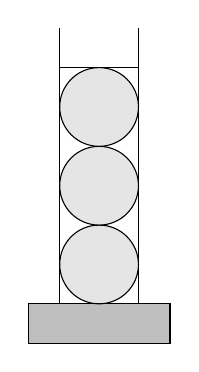
\begin{tikzpicture}
    \draw (0,3.5) -- (0,0) -- (1,0) -- (1,3.5);
    \filldraw [fill = gray!50] (-0.4,0) rectangle (1.4,-0.5);
    \filldraw [fill = gray!20] (0.5,0.5) circle (0.5);
    \filldraw [fill = gray!20] (0.5,1.5) circle (0.5);
    \filldraw [fill = gray!20] (0.5,2.5) circle (0.5);
    \draw (0,3) -- (1,3);
\end{tikzpicture}
\end{center}
\item 在四棱锥$A-BCDE$中, 已知$AD\perp\text{底面}BCDE$, $AC\perp BC$, $AE\perp BE$, 若$\angle CBE=90^\circ$, $CE=\sqrt 3$, $AD=1$, 求$B,D$两点在棱锥$A-BCDE$外接球表面的球面距离.
\begin{center}
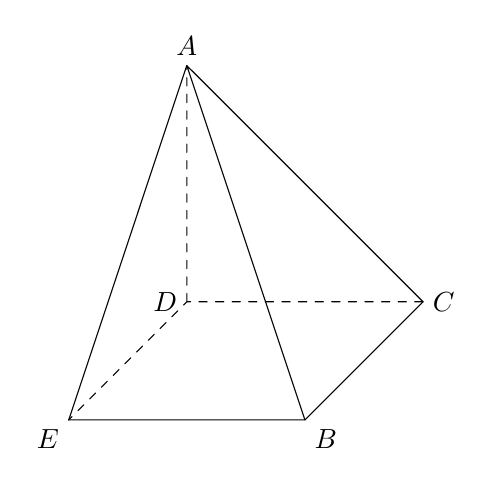
\begin{tikzpicture}[>=latex, line cap = round, line join = round, scale = 3]
    \draw (0,0) node [below left] {$E$} -- (1,0) node [below right] {$B$} --++ (45:{sqrt(2)/2}) node [right] {$C$} coordinate (C);
    \draw [dashed] (C) --++ (-1,0) node [left] {$D$} coordinate (D) -- (0,0) (D) --++ (0,1) node [above] {$A$} coordinate (A);
    \draw (A) -- (0,0) (A) -- (C) (A) -- (1,0);
\end{tikzpicture}
\end{center}
\item 已知$SA$、$SB$是圆锥$SO$的两条母线, $O$是底面圆的圆心, 底面圆的半径为$10$, $C$是$SB$中点, $\angle AOB=60^\circ$, $AC$与底面所成角为$45^\circ$, 求此圆锥的侧面积和体积.
% 第45讲 6+3+4
\item 已知长方体$ABCD-A_1B_1C_1D_1$中, $AB=BC=4$, $CC_1=2$, 则直线$BC_1$和平面$DBB_1D_1$所成角的大小为\blank{50}.
\item 设$ABCD$是一个正方形, $PA\perp$平面$ABCD$, $PA=AB$, 则:\\
(1) 直线$AB$与$PC$所成的角的大小为\blank{50};\\
(2) 直线$PC$与平面$ABCD$所成的角的大小为\blank{50};\\
(3) 二面角$P-BC-A$的大小为\blank{50}.
\item 棱长为$1$的正四面体$ABCD$中, $E,F,G$分别是棱$AB,AC,AD$的中点.\\
(1) 点$A$和平面$BCD$的距离为\blank{50};\\
(2) 直线$EF$和平面$BCD$的距离为\blank{50};\\
(3) 平面$EFG$和平面$BCD$的距离为\blank{50};\\
(4) 异面直线$AD$和$BC$的距离为\blank{50}.
\item 在正四棱锥$P-ABCD$中, 若侧面与底面所成二面角的大小为$60^\circ$, 则异面直线$PA$与$BC$所成角的大小为\blank{50}.
\item 如图, 有一种多面体的饰品, 其表面由$6$个正方形和$8$个正三角形组成, 直线$AB$与$CD$所成角的大小是\blank{50}.
\begin{center}
    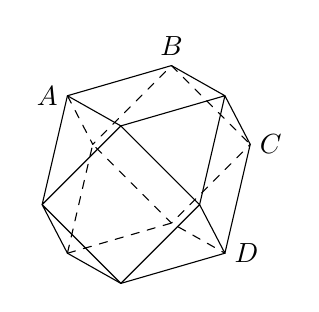
\begin{tikzpicture}[>=latex, line cap = round, line join = round,scale =0.5]
        \draw (0,0) coordinate(M) (4,0) coordinate (N) (N) ++ (50:2) coordinate (P) (M) ++ (50:2) coordinate (Q);
        \draw (M) ++ (0,4) coordinate (M1) (N) ++ (0,4) coordinate (N1) (P) ++ (0,4) coordinate (P1) (Q) ++ (0,4) coordinate (Q1);
        \draw ($(N)!0.5!0:(P)$) coordinate (D) node [right] {$D$} -- ($(M)!0.5!0:(N)$) coordinate (D1) -- ($(M)!0.5!0:(Q)$) coordinate (D2);
        \draw [dashed] (D2) -- ($(P)!0.5!0:(Q)$) coordinate (D3) -- (D);
        \draw ($(P)!0.5!0:(P1)$) coordinate (C) node [right] {$C$} -- (D) -- ($(N)!0.5!0:(N1)$) coordinate (C1) -- (D1) -- ($(M)!0.5!0:(M1)$) coordinate (C2) -- (D2);
        \draw [dashed] (D2) -- ($(Q1)!0.5!0:(Q)$) coordinate (C3) -- (D3) -- (C);
        \draw ($(N1)!0.5!0:(P1)$) coordinate (A1) -- ($(P1)!0.5!0:(Q1)$) coordinate (B) node [above] {$B$} -- ($(M1)!0.5!0:(Q1)$) coordinate (A) node [left] {$A$} 
        -- ($(M1)!0.5!0:(N1)$) coordinate (B1) --  cycle;
        \draw (C) -- (A1) -- (C1) -- (B1) -- (C2) -- (A);
        \draw [dashed] (A) -- (C3) -- (B) -- (C);  
    \end{tikzpicture}
\end{center}
\item 山坡与平面成$30^\circ$角, 坡面上有一条与坡脚水平线成$30^\circ$的直线小路. 某人沿小路上坡走了一段路程后升高了$100$米, 则此人行走的路程为\blank{50}米.
\item 已知正三棱锥$P-ABC$的体积为$72\sqrt 3$, 侧面与底面所成的二面角的大小为$60^\circ$.
\begin{center}
    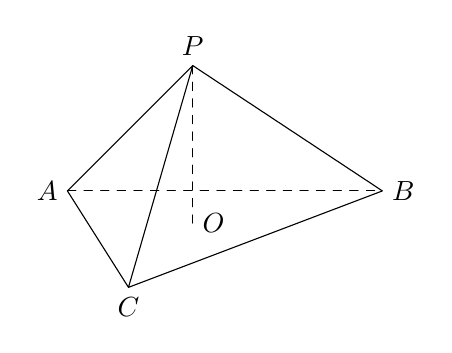
\begin{tikzpicture}[>=latex, line cap = round, line join = round]
        \draw (0,0) coordinate (A) node [left] {$A$} (4,0) coordinate (B) node [right] {$B$};
        \draw (2,0) ++ (225:{sqrt(3)}) coordinate (C) node [below] {$C$};
        \draw (2,0) ++ (225:{sqrt(3)/3}) coordinate (O) node [right] {$O$};
        \draw (O) ++ (0,2) coordinate (P) node [above] {$P$};
        \draw (A) -- (C) -- (B) -- (P) -- (A) (P) -- (C);
        \draw [dashed] (A) -- (B) (P) -- (O);
     \end{tikzpicture}
\end{center}
(1) 证明: $PA\perp BC$;\\
(2) 求底面中心$O$到侧面的距离;\\
(3) 求正三棱锥$P-ABC$的表面积.
\item 如图, 在直三棱柱$ABC-A_1B_1C_1$中, $AA_1=BC=AB=2$, $AB\perp BC$.
\begin{center}
    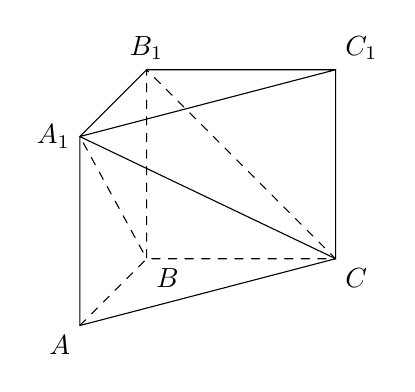
\begin{tikzpicture}[>=latex, line cap = round, line join = round, scale = 0.6]
        \draw (0,0) node [below left] {$A$} coordinate (A) ++ (45:2) node [below right] {$B$} coordinate (B) 
        ++ (4,0) node [below right] {$C$} coordinate (C);
        \draw (A) ++ (0,4) coordinate (A1) node [left] {$A_1$};
        \draw (B) ++ (0,4) coordinate (B1) node [above] {$B_1$};
        \draw (C) ++ (0,4) coordinate (C1) node [above right] {$C_1$};
        \draw (A1) -- (B1) -- (C1) -- cycle;
        \draw (C1) -- (C) -- (A) -- (A1) -- (C);
        \draw [dashed] (A) -- (B) -- (C) -- (B1)-- (B) -- (A1);
    \end{tikzpicture}
\end{center}
(1) 求直线$A_1C$和直线$B_1C_1$所成的角的大小;\\
(2) 求二面角$C-A_1B_1-C_1$的大小;\\
(3) 求点$A$到平面$A_1BC$的距离.
\item 已知$ABCD-A_1B_1C_1D_1$是底面边长为$1$的正四棱柱.
\begin{center}
    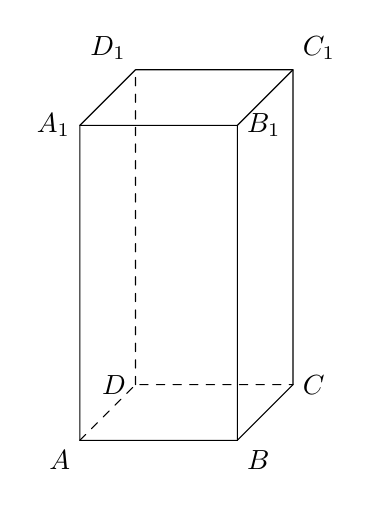
\begin{tikzpicture}[>=latex, line cap = round, line join = round, scale = 2]
        \draw (0,0) node [below left] {$A$} coordinate (A) --++ (1,0) node [below right] {$B$} coordinate (B) --++ (45:{1/2}) node [right] {$C$} coordinate (C)
        --++ (0,2) node [above right] {$C_1$} coordinate (C1)
        --++ (-1,0) node [above left] {$D_1$} coordinate (D1) --++ (225:{1/2}) node [left] {$A_1$} coordinate (A1) -- cycle;
        \draw (A) ++ (1,2) node [right] {$B_1$} coordinate (B1) -- (B) (B1) --++ (45:{1/2}) (B1) --++ (-1,0);
        \draw [dashed] (A) --++ (45:{1/2}) node [left] {$D$} coordinate (D) --++ (1,0) (D) --++ (0,2);
    \end{tikzpicture}
\end{center}
(1) 设$AB_1$与面$A_1B_1C_1D_1$所成的角的大小为$\alpha$, 二面角$A-B_1D_1-A_1$的大小为$\beta$, 试求$\alpha$与$\beta$的一个(非平凡的)等式关系;\\
(2) 若点$C$到平面$AB_1D_1$的距离为$\dfrac 43$, 求该正四棱柱的高;\\
(3) 若正四棱柱的高为$2$, 求四面体$A_1C_1BD$的体积.
\item 在底面边长为$2$的正三棱锥$V-ABC$中, $E$是$BC$的中点, 若三角形$VAE$的面积为$\dfrac 14$, 则侧棱$VA$与底面所成的角的大小为\blank{50}.
\item 在棱长为$2$的正方体$ABCD-A_1B_1C_1D_1$中, $O$为$BD$的中点.\\
(1) 直线$AB_1$与直线$C_1O$所成的角的大小为\blank{50};\\
(2) 直线$BD_1$与平面$A_1B_1C_1D_1$所成的角的大小为\blank{50};\\
(3) 二面角$C_1-BD-A$的大小为\blank{50}.
\item 在棱长为$2$的正方体$ABCD-A_1B_1C_1D_1$中, $O$为$BD$的中点.\\
(1) 点$B$到平面$AB_1D_1$的距离为\blank{50};\\
(2) 直线$C_1O$和平面$AB_1D_1$的距离为\blank{50};\\
(3) 平面$AB_1D_1$和平面$C_1BD$的距离为\blank{50};\\
(4) 异面直线$BD$与$CC_1$的距离为\blank{50}.
\item 在四棱锥$P-ABCD$中, 底面是边长为$2$的菱形. $\angle DAB=60^\circ$, 对角线$AC$与$BD$相交于点$O$, $PO\perp$平面$ABCD$, $PB$与平面$ABCD$所成的角的大小为$60^\circ$.
\begin{center}
    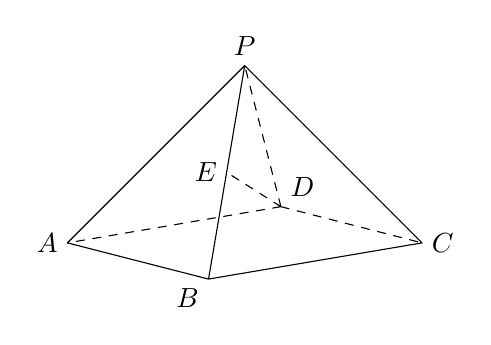
\begin{tikzpicture}[>=latex, line cap = round, line join = round, scale = 1.3]
        \draw ({-sqrt(3)},0) coordinate (A) node [left] {$A$};
        \draw ({sqrt(3)},0) coordinate (C) node [right] {$C$};
        \draw (45:0.5) coordinate (D) node [above right] {$D$};
        \draw (225:0.5) coordinate (B) node [below left] {$B$};
        \draw (0,{sqrt(3)}) coordinate (P) node [above] {$P$};
        \draw ($(P)!0.5!(B)$) coordinate (E) node [left] {$E$};
        \draw (A) -- (B) -- (C) -- (P) -- cycle (P) -- (B);
        \draw [dashed] (D) -- (A) (D) -- (E) (D) -- (C) (D) -- (P);
    \end{tikzpicture}
\end{center}
(1) 求四棱锥$P-ABCD$的体积;\\
(2) 若$E$是$PB$的中点, 求异面直线$DE$与$PA$所成的角的大小.
% 第46讲 8+3+7

\item 用``$\subseteq$''连接集合$\mathbf{Z}$、$\mathbf{Q}$、$\mathbf{R}$、$\mathbf{C}$:\blank{50}.
\item 设复数$z=1-2\mathrm{i}$, 则复数$z-\overline{z+1}=$\blank{50}.
\item 已知$a$是实常数, 则$\dfrac{a+\mathrm{i}}{1+\mathrm{i}}$的虚部$\mathrm{Im}\dfrac{a+\mathrm{i}}{1+\mathrm{i}}=$\blank{50}.
\item 若复数$z$满足$z=\mathrm{i}(2-z)$, 则$z=$\blank{50}.
\item 已知$2z+|z|=1-2\mathrm{i}$, 则复数$z=$\blank{50}.
\item 若纯虚数$z$的模为$2$, 则$z^2=$\blank{50}.
\item 求值: $|\dfrac{(1-\mathrm{i})^{10000}(3-4\mathrm{i})^2}{(-\sqrt{3}+\mathrm{i})^{5000}}|$.
\item 判断下列命题的真假, 对于假命题请至少举一个反例.
\begin{center}
    \begin{tabular}{|c|c|p{.25\textwidth}<{\centering}|}
        \hline
        命题 & 填``真''或``假'' & 反例\\ \hline
        (1) 复数$z$是实数的充要条件是$z-\overline z=0$.	& & \\ \hline
        (2) 复数$z$是纯虚数的充要条件是$z+\overline z=0$. & & \\ \hline
        (3) $z+\overline{z}$和$z\cdot \overline{z}$都是实数. & & \\ \hline
        (4) 已知$|z|=2$, 那么$z=\pm 2$或$\pm 2\mathrm{i}$. & & \\ \hline
    \end{tabular}
\end{center}
\item 求当$a$为何实数时, 复数$z=\dfrac{a^2+a-30}{a+2}+(a^2-3a-10)\mathrm{i}$分别是:\\
(1) 实数;\\
(2) 虚数;\\
(3) 纯虚数;\\
(4) 零.
\item 已知复数$w$满足$w-4=(3-2w)\mathrm{i}$, $z=\dfrac 5w+|w-2|$, 求$|z|$.
\item 已知$z$是虚数, $w=z+\dfrac{1}{z}$是实数, 且$-1<w<2$.\\
(1) 求$|z|$的值及$z$的实部取值范围;\\
(2) 设$u=\dfrac{1-z}{1+z}$, 求证: $u$为纯虚数;\\
(3) 求$w-u^2$的最小值.
\item 复数$2-3\mathrm{i}$的虚部为\bracket{20}.
\fourch{$-3$}{$-3\mathrm{i}$}{$3$}{$3\mathrm{i}$}
\item 若复数$z$满足$z+2\overline z=3-\mathrm{i}$, 则$z=$\blank{50}.
\item 设$b$是实数, 若$\dfrac{1+\mathrm{i}}{2+b\mathrm{i}}+\dfrac 12$的实部与虚部相等, 则$b=$\blank{50}.
\item 设$a$是实数, 若$|\dfrac{(1+\mathrm{i})^3(a-\mathrm{i})^2}{\sqrt{2}(a-3\mathrm{i})^2}|=\dfrac 32$, 则$a=$\blank{50}.
\item 下列命题中正确的有:\blank{50}.\\
(1) 设$z_1,z_2$为复数, 若$z_1^2+z_2^2=0$, 则$z_1+z_2=0$;\\
(2) 设$z_1,z_2$为复数, $z_1\cdot z_2=0$的充要条件为$z_1=0$或$z_2=0$;\\
(3) 若$z_1+z_2>0$, 那么$z_1>-z_2$;\\
(4) 若$|z|\le 1$, 则$-1\le z\le 1$;\\
(5) 若$z\in \mathbf{C}$, 那么$|z^2|=|z|^2$;\\
(6) 若$z\in \mathbf{C}$, 那么$|z|=\sqrt{z^2}$.
\item 已知虚数$z$使得$m=z+\dfrac 4z$是实数.\\
(1) 求$|z|$的值;\\
(2) 求$m$的取值范围;\\
(3) 若$(z+2)(1+\mathrm{i})$是纯虚数, 求$z$的值.\\
\item 已知$|z_1|=2$, $|z_2|=3$, $|z_1+z_2|=4$, 求 $|z_1-2z_2|$.

% 第47讲 8+2+7

\item 复数$z$与$\overline z$在复平面内对应的点\bracket{20}.
\fourch{关于原点对称}{关于$x$轴对称}{关于$y$轴对称}{关于直线$y=x$对称}
\item 若复数$z_1$、$z_2$满足$z_1+z_2=0$, 则$z_1$、$z_2$在复平面上对应的点$Z_1$、$Z_2$\bracket{20}.
\fourch{关于原点对称}{关于$x$轴对称}{关于$y$轴对称}{关于直线$y=x$对称}
\item 满足$\begin{cases} |z-\mathrm{i}|\le 1, \\ \mathrm {Re}z\ge 0 \end{cases}$的复数、在复平面内对应点所构成图形的面积为\blank{50}.
\item 平行四边形$ABCD$的三个顶点$A,B,C$依次对应复数$z_1=0$, $z_2=1+\mathrm{i}$, $z_3=-1+2\mathrm{i}$, 则点$D$对应的复数为\blank{50}.
\item 设$z=a+b\mathrm{i}$($a,b\in\mathbf{R}$), 则$\mathrm{i}\cdot \overline{z}$所表示的点、关于直线$y=x$对称的点的复数表示为\blank{50}.
\item 满足下列条件的复数$z$所对应点的轨迹是什么? 在空格内填入轨迹类型和直角坐标系下方程.\\
例子: (0) $|z|=1$: 圆$x^2+y^2=1$;\\
(1) $|z-\mathrm{i}|=|z+\mathrm{i}|$:\blank{50};\\
(2) $|z+1|=1$:\blank{50};\\
(3) $|z-5|+|z+5|=12$:\blank{50};\\
(4) $|z-1|+|z+1|=2$:\blank{50};\\
(5) $|z-2\mathrm{i}|-|z+2\mathrm{i}|=2$:\blank{50}.
\item 已知$|z_1|=1$, $|z_2|=\sqrt{3}$, $|z_1-z_2|=2$, 则$|z_1+z_2|=$\blank{50}.
\item 已知$|z|=|z-1|=1$, 则$z=$\blank{50}.
\item (1) 已知$|z|=1$, 求$|z-2|$的取值范围;\\
(2) 已知$|z-\mathrm{i}|=3$, 求$|z+1|$的取值范围.
\item 设复数$z$满足$|z+1-2\mathrm{i}|=3$, 复数$w=4z-\mathrm{i}+1$, 求复数$w$对应点的轨迹.
\item 由方程:$|z|^2-8|z|+15=0$所确定的复平面内对应的点所组成的图形是\bracket{20}.
\fourch{四个点}{四条直线}{一个圆}{ 两个圆}
\item 已知$|z-2|=|z-1+\mathrm{i}|$, 则复数$z$在复平面上所对应的点$Z$的轨迹是\blank{50}.
\item 满足方程$z\overline{z}-z-\overline{z}=8$的复数$z$在复平面上所对应的点的轨迹是\blank{50}.
\item 设复数$z$满足$|z+1|+|z-1|=2$, 则$|z-4-\mathrm{i}|$的最小值为\blank{50}.
\item 若集合$A=\{z||z+5\mathrm{i}|-|z-5\mathrm{i}|=8\}$, $B=\{z||z|=4\}$, 则$A\cap B=$\blank{50}.
\item 已知复数z满足$|z-3+4\mathrm{i}|=2$,\\
(1) 求$|z+1|$的取值范围;\\
(2) 求出使$|z+1|$取最大值的$z$的值.
\item 已知复数$z$满足$|z|=2$, 求复数$w=\dfrac{1+z}z$在复平面内的对应点的轨迹.
% 第48讲 8+3+7


\item 负实数$a$的平方根为\blank{50}.
\item $8$的立方根为\blank{50}.
\item 计算: $1+\mathrm{i}+\mathrm{i}^2+\cdots+\mathrm{i}^{100}=$\blank{50}.
\item 设$\omega=-\dfrac 12+\dfrac{\sqrt 3}2\mathrm{i}$, 则$1+\omega+\omega^2+\omega^3+\cdots+\omega^{2000}=$\blank{50}.
\item 计算: $(1+\mathrm{i})^{10000}=$\blank{50}.
\item (1) $2x^2+4x+1=0$的解为\blank{50};\\
(2) 复数集中分解因式: $2x^2+4x+1=$\blank{50}.
\item 已知关于$x$的实系数一元二次方程$ax^2+bx+c=0\ (a\ne 0)$在复数集中的两个根为$\alpha,\beta$, 下列命题中正确的有\blank{50}.\\
\textcircled{1} $\alpha$和$\beta$互为共轭复数;\\
\textcircled{2} $\alpha +\beta =-\dfrac ba$, $\alpha \beta =\dfrac ca$;\\
\textcircled{3} $\alpha$和$\beta$分别为$\dfrac{-b\pm \sqrt{b^2}-4ac}{2a}$;\\
\textcircled{4} $|\alpha -\beta|^2=(\alpha-\beta)^2$;\\
\textcircled{5} $ax^2+bx+c=a(x-\alpha)(x-\beta)$.
\item 求$-\dfrac{13}4+2\sqrt 3\mathrm{i}$的平方根.
\item 设$p,q\in \mathbf{R}$, 若关于$x$的方程$2x^2+px+q=0$的一个根为$-3+2\mathrm{i}$, 求$p,q$的值.
\item 设$m$是实数, 关于$x$的方程$x^2-mx+1=0$的两个复数根为$\alpha,\beta$. 若$|\alpha-\beta|=1$, 求$m$的值.
\item 设$m$是实数, 若关于$x$的方程$2x^2+3mx+m^2-m=0$至少有一个模为$1$的根, 求$m$的值.
\item 实数$-2$的平方根为\blank{50}.
\item 实数$-1$的立方根为\blank{50}.
\item 若复数$a+b\mathrm{i}$($a,b\in \mathbf{R}$)是关于$x$的实系数方程$x^2+px+q=0$的两根, 则$p=$\blank{50}, $q=$\blank{50}.
\item 计算: $\mathrm{i}\cdot\mathrm{i}^2\cdot\mathrm{i}^3\cdot \cdots \cdot \mathrm{i}^{100}=$\blank{50}.
\item 设$m$是实数, 关于$x$的方程$x^2-2\sqrt 2x+m=0$的两个复数根为$\alpha,\beta$.\\
(1) 若$|\alpha-\beta|=3$, 求实数$m$的值;\\
(2) 若$|\alpha|+|\beta|=3$, 求实数$m$的值.
\item 设$m$是实数, 若$\alpha$是实系数一元二次方程$mx^2+x+1=0$的根, 且满足$|\alpha+1|=1$, 求$m$的取值范围.
\item 已知关于$x$的方程$x^2+(4+\mathrm{i})x+3+p\mathrm{i}=0$($p\in \mathbf{R}$)有实数根, 求$p$的值, 并解这个方程.
% 第49讲 5+3+5

\item 若矩阵$\begin{pmatrix}a & b \\ c & d\end{pmatrix}$为$n$阶单位阵, 则$a-b-c+d+n=$\blank{50}.
\item 方程组$\begin{cases} 2x+y=7, \\ x-y=2 \end{cases}$的系数行列式的值为\blank{50}, 系数矩阵的行向量为\blank{50}.
\item 行列式$\begin{vmatrix}1 & 2 & 0 \\ 1 & 5 & 1 \\ 1 & 8 & 0 \end{vmatrix}=$\blank{50}.
\item 在三阶行列式$\begin{vmatrix}1 & 2 & 3 \\4 & 5 & 6  \\7 & 8 & -9 \end{vmatrix}$中, 元素$6$的余子式为\blank{50}, 元素$8$的代数余子式的值为\blank{50}.
\item 关于$x$、$y$的方程组$\begin{cases} mx+2y=m+4, \\ 2x+my=m \end{cases}$无解, 则实数$m=$\blank{50}.

\item 设$m$是实数, 解关于$x,y$的方程组$\begin{cases} mx+2y=m, \\ x+(m-1)y=-m. \end{cases}$
\item 已知关于$x,y,z$的方程组$\begin{cases} x+y+z=1, \\ x+y+az=1, \\ x+ay+a^2z=2, \end{cases}$其中$a\in \mathbf{R}$.\\
(1) 若关于$x$、$y$的方程组$\begin{cases} a_1x+b_1y=c_1, \\ a_2x+b_2y=c_2 \end{cases}$可以用矩阵记号$\begin{pmatrix}
 a_1 & b_1 \\ a_2 & b_2  \end{pmatrix}\begin{pmatrix}    x  \\ y  \end{pmatrix}=\begin{pmatrix} c_1 \\ c_2 \end{pmatrix}$来表示, 请试给出上述三元一次方程组的矩阵表示;\\
(2) 用行列式的方法解此方程组.
\item 已知平面直角坐标系内点$A(0,3)$, 点$B(2,0)$, 点$C(5,\lambda)$.\\
(1)	若三角形$ABC$面积为$10$, 求$\lambda$的值;\\
(2)	若$A,B,C$三点共线, 求$\lambda$的值.
\item 行列式$\begin{vmatrix} 1 & 3 & 0  \\ 4 & 5 & 1  \\ 7 & 8 & 2 \end{vmatrix}$中, 元素$4$的余子式的值为\blank{50}, 元素$3$的代数余子式的值为\blank{50}.
\item 将 $a\begin{vmatrix} 1 & 2 \\0 & 4 \end{vmatrix}+b \begin{vmatrix}
-1 & 3  \\ 0 & 4 \end{vmatrix}+c \begin{vmatrix}
-1 & 3  \\ 1 & 2 \end{vmatrix}$化为一个三阶行列式: $\begin{vmatrix}a & -1 & 3 \\ \blank{10} & \blank{10} & \blank{10} \\ \blank{10} & \blank{10} & \blank{10}\end{vmatrix}$.
\item 若关于$x$、$y$的方程组$\begin{cases} mx+y=-1,\\ x+my=1 \end{cases}$有解, 则实数$m$的取值范围为\blank{50}.
\item 关于$x,y,z$的方程组$\begin{cases} x+y+az=1, \\ x+ay+z=a, \\ x-y+z=3 \end{cases}$的增广矩阵是\blank{50}; 若此方程组有唯一解, 则实数a的取值范围为\blank{50}.
\item 设$m$是实数, 用行列式的方法解关于$x$、$y$的方程组$\begin{cases} (m+1)x-(2m-1)y=3m, \\ (3m+1)x-(4m-1)y=5m+4. \end{cases}$
% 第50讲 10+3+9

\item 若$m\in \mathbf{N}^*$, $m<27$, 则$(27-m)(28-m)\cdots (34-m)=$\blank{50}(用排列数表示).
\item $540$的不同的正约数共有\blank{50}个, 这些正约数中是$3$的倍数的有\blank{50}个.
\item $3000$和$8000$之间有\blank{50}个能被5整除的且在数位上无重复数字的数.
\item 平面上有$10$个点, 其中除有$4$个点在同一条直线上外, 不再有其它三点共线的情形, 经过这些点可以确定\blank{50}条直线.
\item 从$5$男$3$女共$8$名学生中选出队长$1$人, 副队长$1$人, 普通队员$2$人组成$4$人志愿者服务队, 要求服务队中至少有$1$名女生, 共有\blank{50}种不同的选法(用数字作答).
\item $(2x-\dfrac 1{\sqrt x})^6$的展开式中第三项的二项式系数为\blank{50}, 第三项的系数为\blank{50}.
\item 化简: (1) $1+2\mathrm{C}_n^1+4\mathrm{C}_n^2+\cdots+2^n\mathrm{C}_n^n=$\blank{50};\\
(2) $\mathrm{C}_3^3+\mathrm{C}_4^3+\mathrm{C}_5^3+\cdots+\mathrm{C}_n^3=$\blank{50}.
\item 随机抽取$9$个同学中, 至少有$2$个同学在同一月出生的概率是\blank{50}(默认每月天数相同, 结果精确到$0.001$).
\item 从一副$52$张扑克牌中随机抽取$4$张牌.\\
(1) 在放回抽取的情形下, $4$张牌都是A的概率为\blank{50};
(2) 在不放回抽取的情形下, $4$张牌都是A的概率为\blank{50}.
\item *已知总体的各个体的值由小到大依次为$2,3,3,7,a,b,12, 13.7,18.3,20$, 且总体的中位数为$10.5$. 若要使该总体的方差最大, 则$a$=\blank{50}, $b$=\blank{50}.
\item 有$3$名男生, $4$名女生, 全体排成一行, 在下列不同的要求下, 分别求不同排列的方法数:\\
(1) 男生必须排在一起;\\
(2) 任意两个男生都不相邻;\\
(3) 甲不在最左边, 乙不在最右边;\\
(4) 甲必须站在乙的左方(不一定相邻);\\
(5) 其中甲、乙、丙三人从左至右的顺序不变(都不一定相邻).
\item 求二项式$(2+x^2)^{32}$展开式中,\\
(1) 二项式系数最大的项;\\
(2) 系数最大的项;\\
(3) 所有项的系数之和.
\item 某中学共有学生$2000$名, 各年级男、女生人数如下表.
\begin{center}
    \begin{tabular}{|c|c|c|c|}
        \hline
        & 一年级 & 二年级 & 三年级\\ \hline
        女生 & $373$ & $x$ & $y$ \\ \hline
        男生 & $377$ & $370$ & $z$ \\ \hline
    \end{tabular}
\end{center}
已知在全校学生中随机抽取$1$名, 抽到二年级女生的概率是0.19.\\
(1) 求$x$的值;\\
(2) 现用分层抽样的方法在全校抽取$48$名学生, 问应在三年级抽取多少名?\\
(3) 已知$y\ge 245$, $z\ge 245$, 求三年级中女生比男生多的概率.
\item 已知$\mathrm{C}_{18}^{2x}=\mathrm{C}_{18}^{x+3}$, 则$x$=\blank{50}.
\item 用$0$、$1$、$2$、$3$、$4$、$5$组成的无重复数字的数中比$240135$大的数有\blank{50}个.
\item 甲、乙、丙三人值周一至周六的班, 每人值两天班, 若甲不值周一、乙不值周六, 则可排出不同的值班表数为\blank{50}.
\item 在$(\sqrt[3]x-\dfrac 1{2\cdot \sqrt[3]x})^{10}$的二项展开式中, 常数项是\blank{50}; 含$x^2$项的二项式系数是\blank{50}; 含$x^2$项的系数是\blank{50}.
\item 设$1+(1+x)+(1+x)^2+\cdots+(1+x)^{2021}=a_0+a_1x+a_2x^2+\cdots +a_{2021}x^{2021}$, 则$a_{100}+a_{101}=$\blank{50}.
\item 已知$a,b\in \{-3,-2,-1,1,2,3\}$且$a\ne b$, 则复数$z=a+b\mathrm{i}$对应点在第二象限的概率为\blank{50}(用最简分数表示).
\item 盒子中装着标有$1,2,3,4$的卡片各两张, 从盒中任取$3$张, 每张卡片被抽到的概率相等, 则抽出的$3$张卡片上的数字互不相同的概率为\blank{50}.
\item 某区有$200$名学生参加数学竞赛, 随机抽取10名学生成绩如下:
\begin{center}
    \begin{tabular}{|c|c|c|c|c|c|c|}
        \hline
        成绩 & $40$ & $50$ & $60$ & $70$ & $80$ & $90$\\ \hline
        人数 & $2$ & $1$ & $2$ & $2$ & $1$ & $2$ \\ \hline        
    \end{tabular}
\end{center}
则总体标准差的点估计值是\blank{50}.(精确到$0.01$)
\item 某学校组织学生参加英语测试, 成绩的频率分布直方图如图所示, 数据的分组依$[20,40)$, $[40,60)$, $[60,80)$, $[80,100)$, 若低于$60$分的人数是$15$人, 则该班的学生人数是\blank{50}.
\begin{center}
\begin{tikzpicture}[>=latex, line cap = round, line join = round, scale = 1.2]
    \draw [->] (-2,0) -- (6.5,0) node [below] {成绩(分)};
    \draw [->] (0,-1) -- (0,3) node [left] {$\dfrac{\text{频率}}{\text{组距}}$};
    \draw (0,0) node [below left] {$O$};
    \draw (1,0) -- (1,0.5) -- (2,0.5);
    \draw (2,0) -- (2,1) -- (3,1);
    \draw (3,0) -- (3,2) -- (4,2) -- (4,0);
    \draw (4,1.5) -- (5,1.5) -- (5,0);
    \draw [dashed] (0,0.5) -- (1,0.5) (0,1) -- (2,1) (0,1.5) -- (4,1.5) (0,2) -- (3,2);
    \foreach \i in {20,40,...,100}
        \draw ({\i/20},0) node [below] {$\i$};
    \foreach \i in {0.005,0.01,0.015,0.02}
        \draw (-1.2,{\i*100}) node [right] {$\i$};
\end{tikzpicture}
\end{center}
\end{enumerate}
\end{document}